%!TEX root = ../my_thesis.tex
\section{Data sample and preselection}
\label{sec:sample_and_selection}

%===============================================================================
The sample of data is passed through the following selection steps:
\begin{enumerate}[noitemsep,topsep=0pt]
	\item stripping and trigger requirements;
	\item a \emph{cut-based} preselection;
	\item vetoes for misidentified backgrounds and wrongly associated \emph{primary vertices} (PVs);
	\item a multivariate classification (MVA);
	\item a final randomised multiple candidate selection.
\end{enumerate}
In what follows, the details of each step are provided.

%===============================================================================
\subsection{Stripping and trigger requirements}
\label{sec:stripping}

Signal $\Bz\to\Dmp\pipm$ candidates are reconstructed using a dedicated stripping line
(called \verb!B02DPiD2HHHBeauty2CharmLine!). Each event is required to have less than
\num{500} long tracks. The criteria that the charged tracks have to
fulfill are listed in Table~\ref{tab:strippingDaughters}.
%
\begin{table}[b!]
	\centering
	\caption{Stripping requirements applied in the selection of charged tracks. The more stringent
	  requirements given in brackets are for the bachelor track. The IP$\chi^2$ is 
          the vertex-fit $\chi^2$ difference for the PV reconstructed with and without the $\Bz$ candidate.}
	\begin{tabular}{cc}
		\toprule
		track $\chi^2/$ndof & $<\num{3.0}$ ($<\num{2.5}$)\\
		momentum $p$ & $>\SI{1}{\GeVc}$ ($>\SI{5}{\GeVc}$)\\
		transverse momentum $\pt$ & $>\SI{100}{\MeVc}$ ($>\SI{500}{\MeVc}$)\\
		IP$\chi^2$ w.r.t. any PV & $>\num{4.0}$\\
		ghost probability & $<\num{0.4}$\\
		\bottomrule
	\end{tabular}
	\label{tab:strippingDaughters}
\end{table}
%
Three of these hadrons have to form a common vertex to build a $\Dmp$ meson. 
Further requirements on the \Dmp~combination are given in
Table~\ref{tab:strippingD}.
%
\begin{table}[htbp]
	\centering
	\caption{Stripping requirements on the three-track combinations forming $\Dmp$ candidates. DOCA is the Distance Of
	  Closest Approach of the daughter particles w.r.t. each other, and
	  DIRA indicates the cosine of the angle between the momentum of the $\Dmp$
	  meson and the direction from the best PV to the decay vertex. The best PV is defined as
	  the vertex with the lowest IP$\chi^2$.}
	\begin{tabular}{cc}
		\toprule
		$\sum$ $\pt(hhh)$ & $>\SI{1800}{\MeVc}$\\
		DOCA & $<\SI{0.5}{\milli\metre}$\\
		$m(hhh)$ & $\in[1769.62,2068.49]\mevcc$\\
		$\Dmp$ vertex $\chi^2/$ndof & $<\num{10.0}$\\
		$\Dmp$ vertex separation $\chisq$ to any PV & $>\num{36}$\\
		$\Dmp$ DIRA & $>\num{0.0}$\\
		\bottomrule
	\end{tabular}
	\label{tab:strippingD}
\end{table}
%
The $\Bz$ candidates are built by combining a $\Dmp$ candidate and a bachelor
particle if the requirements listed in Table~\ref{tab:strippingB} are fulfilled.
Finally, a bagged boosted decision tree (BDT) classifier~\cite{Breiman:1996zz}, which is trained on
simulated data, is applied. A
minimum value of $\num{0.05}$ is required for the output value of the BDT.
%
\begin{table}[htbp]
	\centering
	\caption{Stripping requirements on the $\Dmp\pipm$ combination (before the BDT requirement mentioned in the text).}
	\begin{tabular}{cc}
		\toprule
		$\Bz$ vertex \chisqndf & $<\num{10.0}$\\
		reconstructed $\Bz$ proper decay time $t$ & $>\SI{0.2}{ps}$\\
		IP$\chi^2$ w.r.t.\ the best PV & $<\num{25.0}$\\
		$\Bz$ DIRA & $>\num{0.999}$\\
		\bottomrule
	\end{tabular}
	\label{tab:strippingB}
\end{table}
%
Stripped candidates are then filtered according to how they were selected at the
trigger level: no specific requirements are made at L0; at HLT1, $\B$ candidates
are required to be TOS from the \verb!Hlt1TrackAllL0Decision! trigger line; at
HLT2, $\B$ candidates are required to be TOS from one of the following lines:
\verb!Hlt2Topo2BodyBBDTDecision!, \verb!Hlt2Topo3BodyBBDTDecision! or
\verb!Hlt2Topo4BodyBBDTDecision!. These trigger lines are described in detail in 
Refs.~\cite{LHCb-PUB-2011-003Vava,LHCb-INT-2011-030Vava}.

Figure~\ref{fig:mB_mD_after_stripping} shows the $\Dmp\pipm$ and $K^{\pm}\pimp\pimp$ mass
distributions of the reconstructed candidates after the stripping and trigger
selections. In the $\Dmp\pipm$ mass distribution the $\Bz\to\Dmp\pipm$ signal peak is already visible at
around \SI{5280}{\MeVcc}. The structure at masses lower than the $\B$ peak originates from
partially reconstructed $\Bz\to\D\rho$ and $\Bz\to\Dstar\pi$ decays. The $K^{\pm}\pimp\pimp$
mass distribution features a clearly visible $\Dmp\to K^{\pm}\pimp\pimp$ peak at \SI{1870}{\MeVcc} and
a $D^{*\mp}\to D^0(K^\pm\pimp)\pimp$ peak around \SI{2010}{\MeVcc}.
%
\begin{figure}[t]
	\begin{center}
		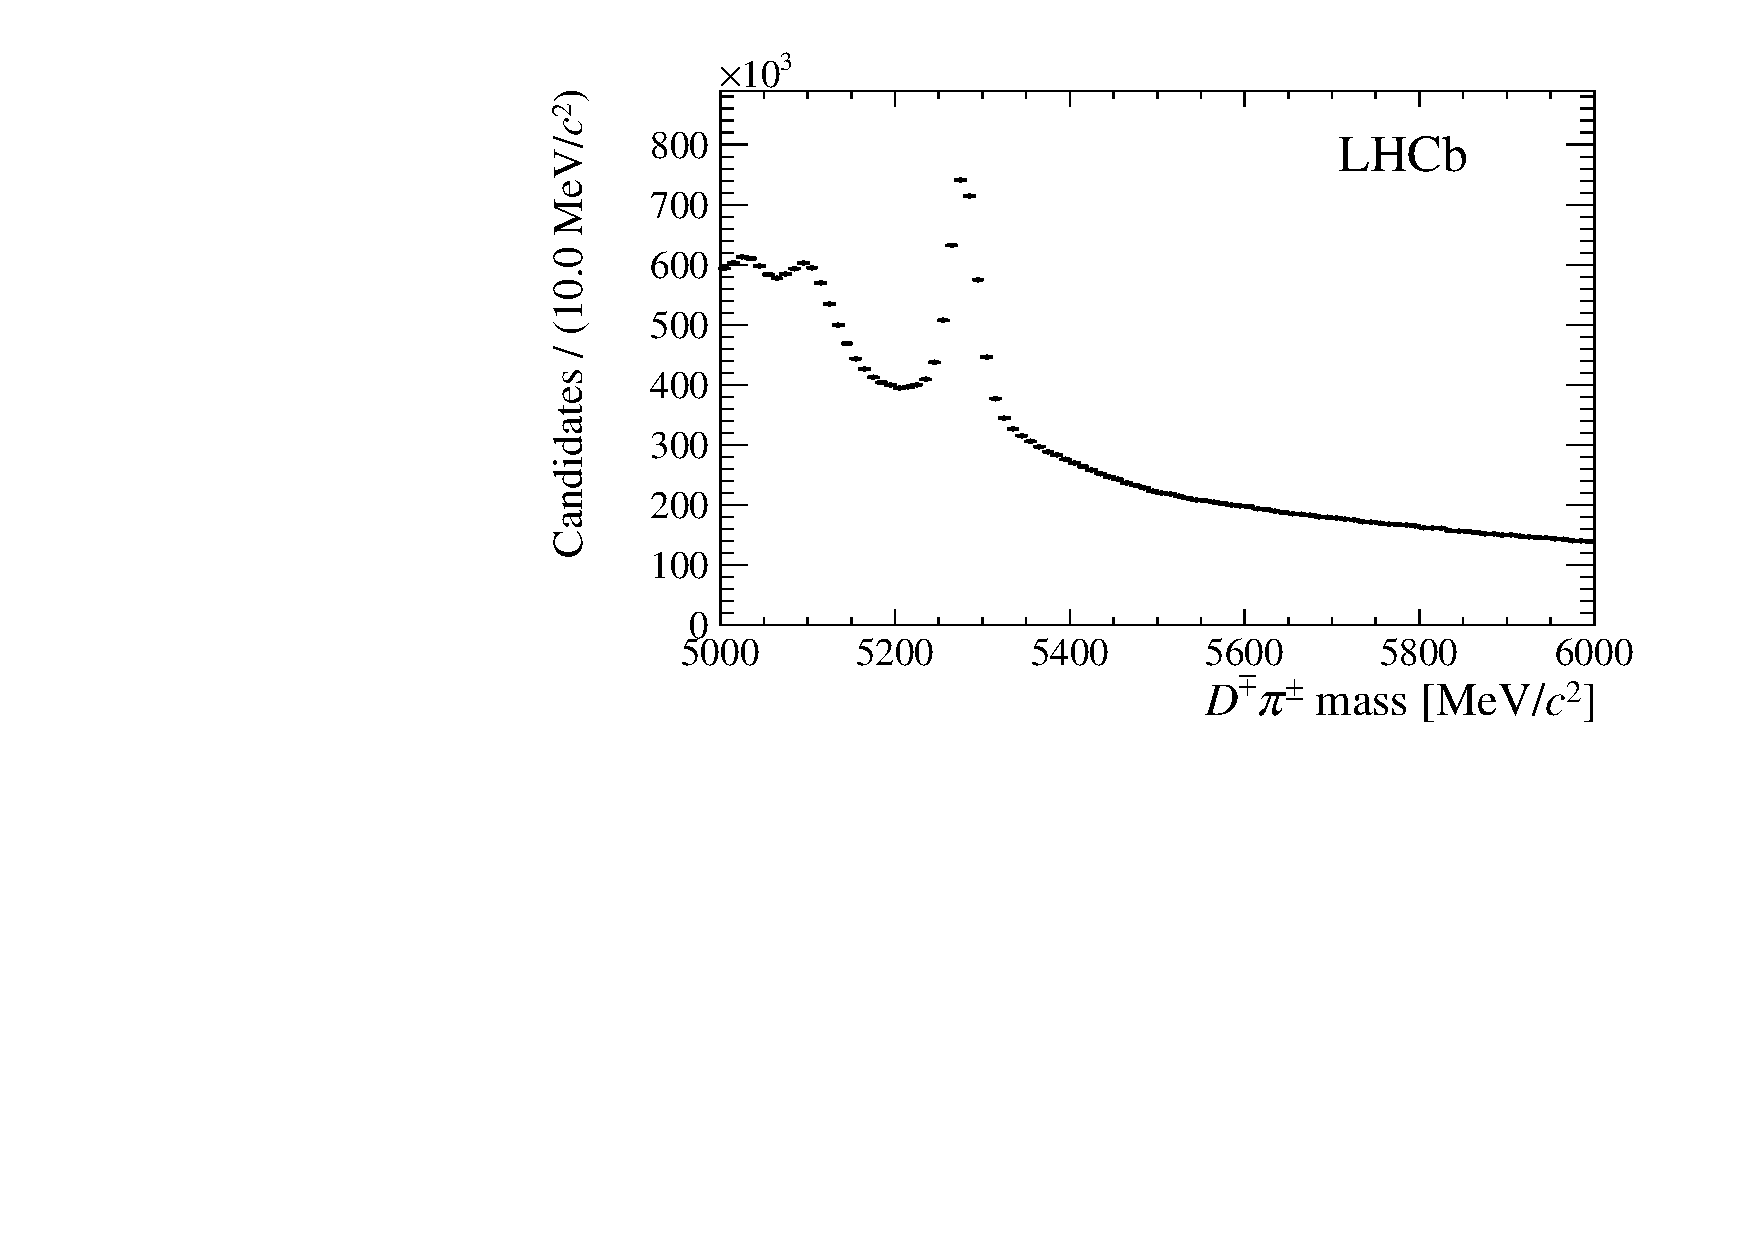
\includegraphics[width=0.49\textwidth]{02Selection/figs/Bmass_afterStrippingAndTrigger.pdf}
		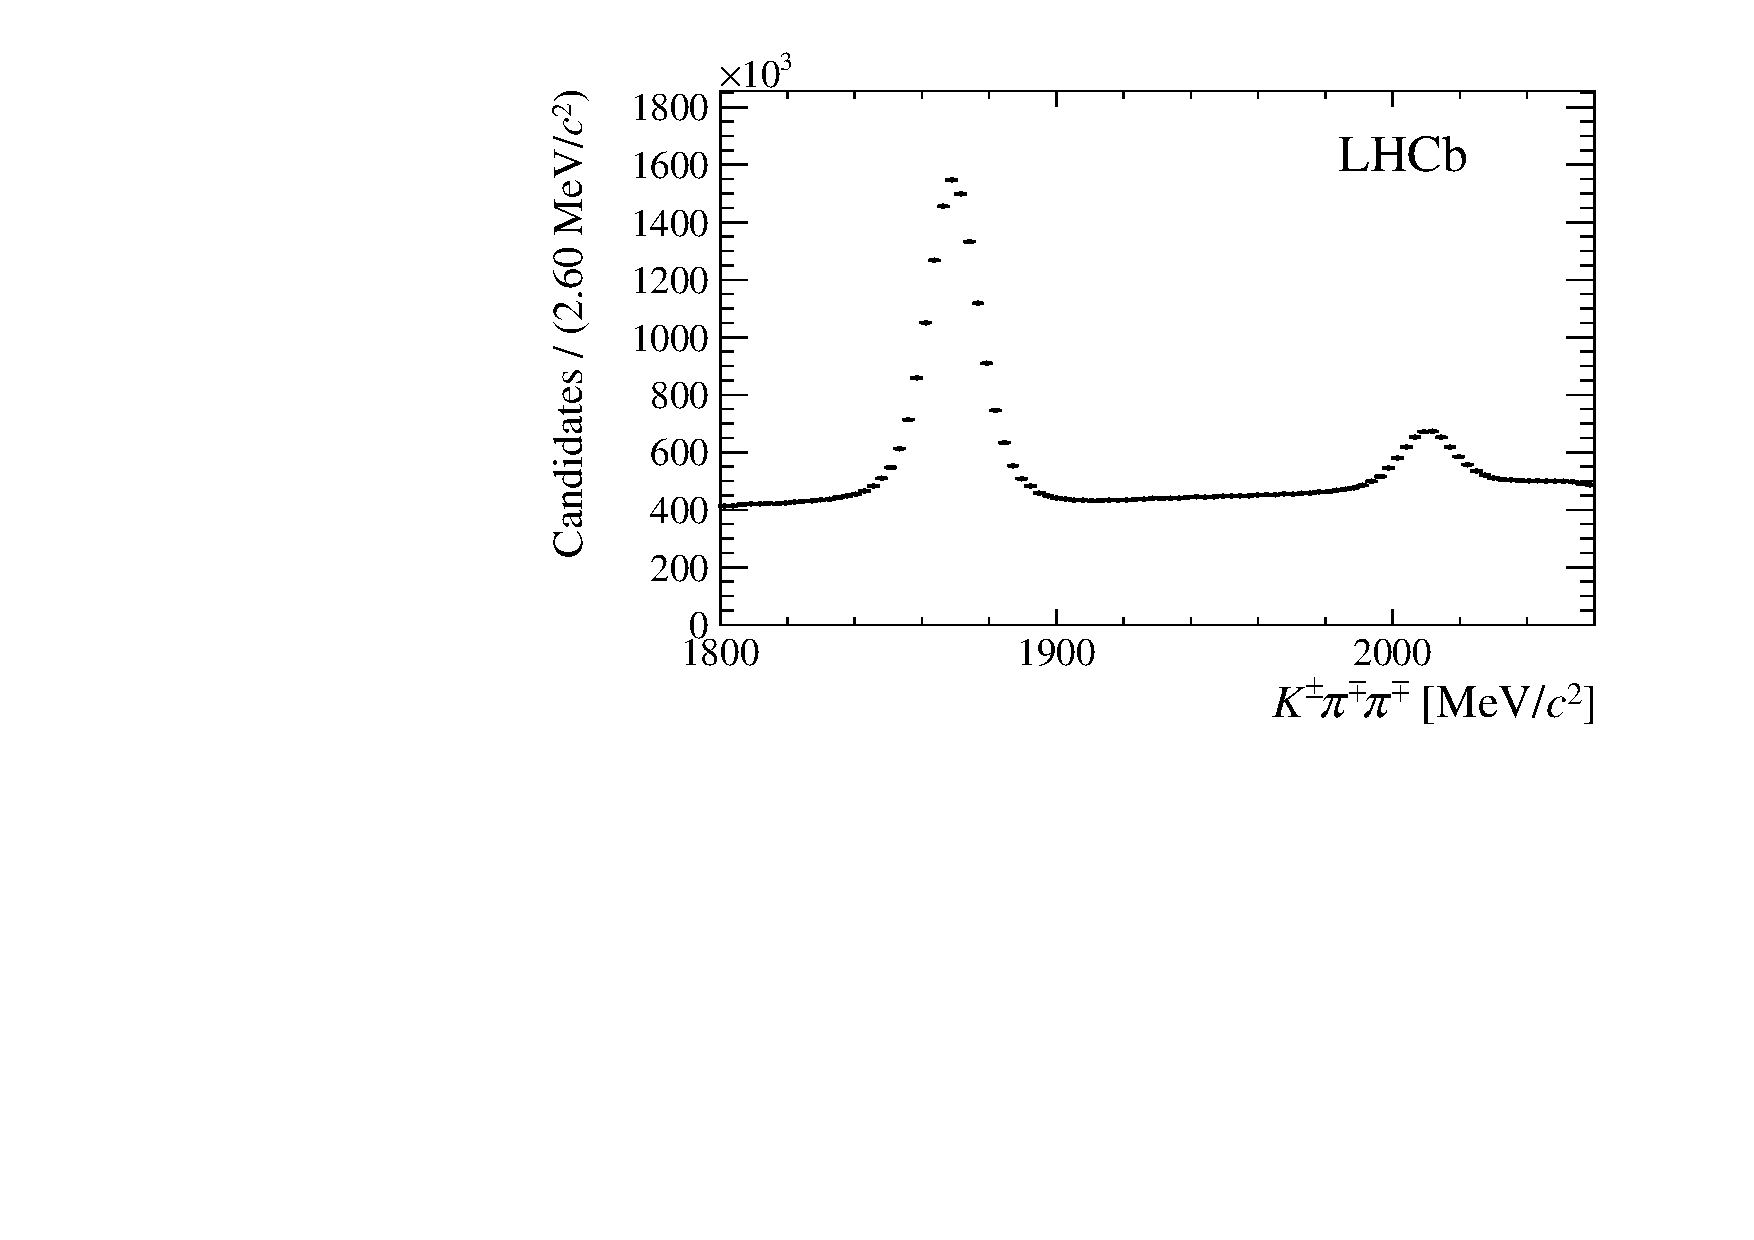
\includegraphics[width=0.49\textwidth]{02Selection/figs/Dmass_afterStrippingAndTrigger.pdf}
	\end{center}
        \vspace{-2mm}
	\caption{$\Dmp\pipm$ and $K^{\pm}\pimp\pimp$ mass distributions of the reconstructed $\Bz\to\Dmp\pipm$, $\Dmp\to K^{\pm}\pimp\pimp$ candidates
	after the stripping and trigger selection.}
	\label{fig:mB_mD_after_stripping}
\end{figure}

%===============================================================================
\subsection{Preselection and sample definitions}
\label{sec:preselection}

Additional preselection criteria (shown in Table~\ref{tab:preselection}) are
applied offline. In order to obtain the correct correlations between the uncertainties
on vertex positions, particle momenta, flight distances, decay times, and
invariant masses, a Kalman filter, known as \verb!DecayTreeFitter! (DTF)~\cite{DTF}, is used. 
The decay-time related observables are derived
from a DTF fit where the position of the primary vertex has been used to
constrain the production vertex of the $\Bz$ meson. To determine the momentum and
the invariant mass of the $\Bz$ meson, the invariant mass of the $\Dmp$ meson is
constrained to the central value of the PDG
($m_{\Dmp}^\text{PDG}=\SI{1869.61}{\MeVcc}$~\cite{PDG}) in a separate DTF
fit.
%
\begin{table}[t]
	\centering
	\caption{Offline preselection requirements.}
	\begin{tabular}{cc}
		\toprule
		$\Bz$ candidate decay time & $>\SI{0.2}{ps}$\\
		$\left|m(\Kpm\pimp\pimp)-m_{\Dmp}^\text{PDG}\right|$ & $<\SI{35}{\MeVcc}$\\
		$\PIDK$ for pions & $<+8$ from $\Dmp$\\
		$\PIDK$ for kaon & $>-2$ from $\Dmp$\\
		\bottomrule
	\end{tabular}
	\label{tab:preselection}
\end{table}
%
The $\PIDK$ variable of Eq.~\ref{eq:pidx} is used to identify the kaon and
the pions from the $\Dmp$ decays, and to identify the bachelor pion from the $\Bz$
decay. The requirement on the $\PIDK$ of the bachelor pion defines two samples
of candidates: the so-called \emph{pion sample }($\PIDK\leq 5$)
and the so-called \emph{kaon sample} ($\PIDK>5$). This distinction will be
useful in the fit to the $\Bz$ mass distribution described in Sec.~\ref{sec:massfit} for determining the sample
composition. 
All the following selection steps are applied to both the pion and kaon samples.

%===============================================================================
\subsection{Vetoes against physics backgrounds}
\label{sec:vetoes}

Misidentification of muons, kaons and protons as pions leads to exclusive backgrounds. 
These are suppressed by means of explicit \emph{vetoes}. In order to 
reduce contributions from semileptonic decays such as
$\Bz\to\Dm\left(\to\Kp\pim\pim\right)\mu^{+}\nu_{\mu}$, the bachelor pion is required
to have no hits in the muon chambers.
A $\proton\to\pion$ mis-identification can lead to background contributions from
$\Lb\to\Lambda_c^{+}\left(\to\Km\pip p\right)\pim$. To reduce these
contributions, the proton mass hypothesis is applied separately to both pion candidates
from the $\Dpm$ final state. The invariant mass of the three hadrons is
recalculated and if the candidate is inside a \SI{\pm30}{\MeVcc} (\SI{\pm50}{\MeVcc}) window around the
$\Lambda_c^{+}$ mass, $m_{\Lambda_c^{+}} = \SI{2286.46}{\MeVcc}$~\cite{PDG}, it is
required to have PID$p<-8.0$ (PID$p<-5.0$). 
A plot showing the distributions before
and after applying the veto is given in Fig. \ref{fig:lambdaveto}. This requirement
shows a signal efficiency of \SI{93.48\pm0.06}{\percent}. The rejection of
$\Lb\to\Lambda_c^{+}\pim$ is checked with simulation. 
After stripping and preselection alone, \SI{99.720\pm0.004}{\percent} of the
$\Lb\to\Lambda_c^{+}\pim$ decays are rejected, and this veto rejects
\SI{76.6\pm0.6}{\percent} of the remaining $\Lb\to\Lambda_c^{+}\pim$ decays.

\begin{figure}[t]
	\begin{center}
		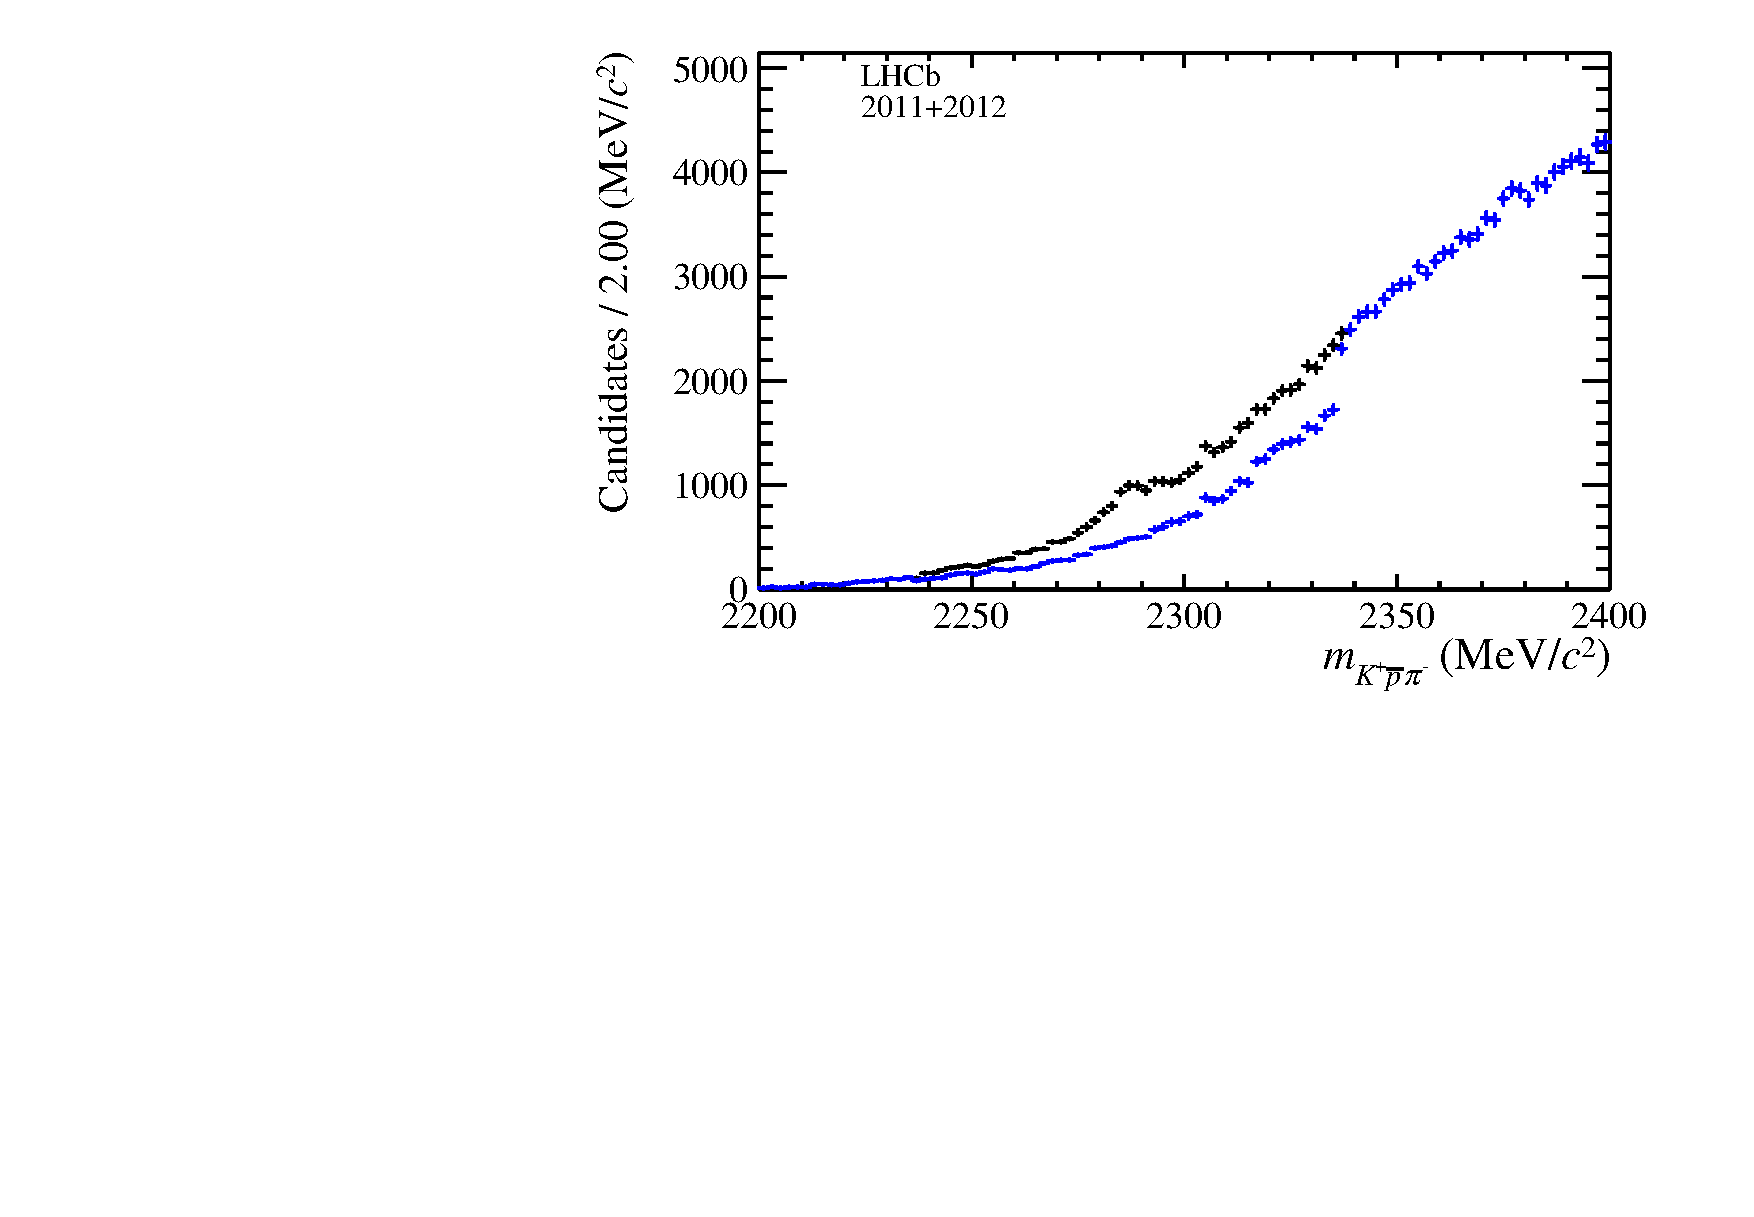
\includegraphics[width=0.45\textwidth]{02Selection/figs/LcHypo1.pdf}
		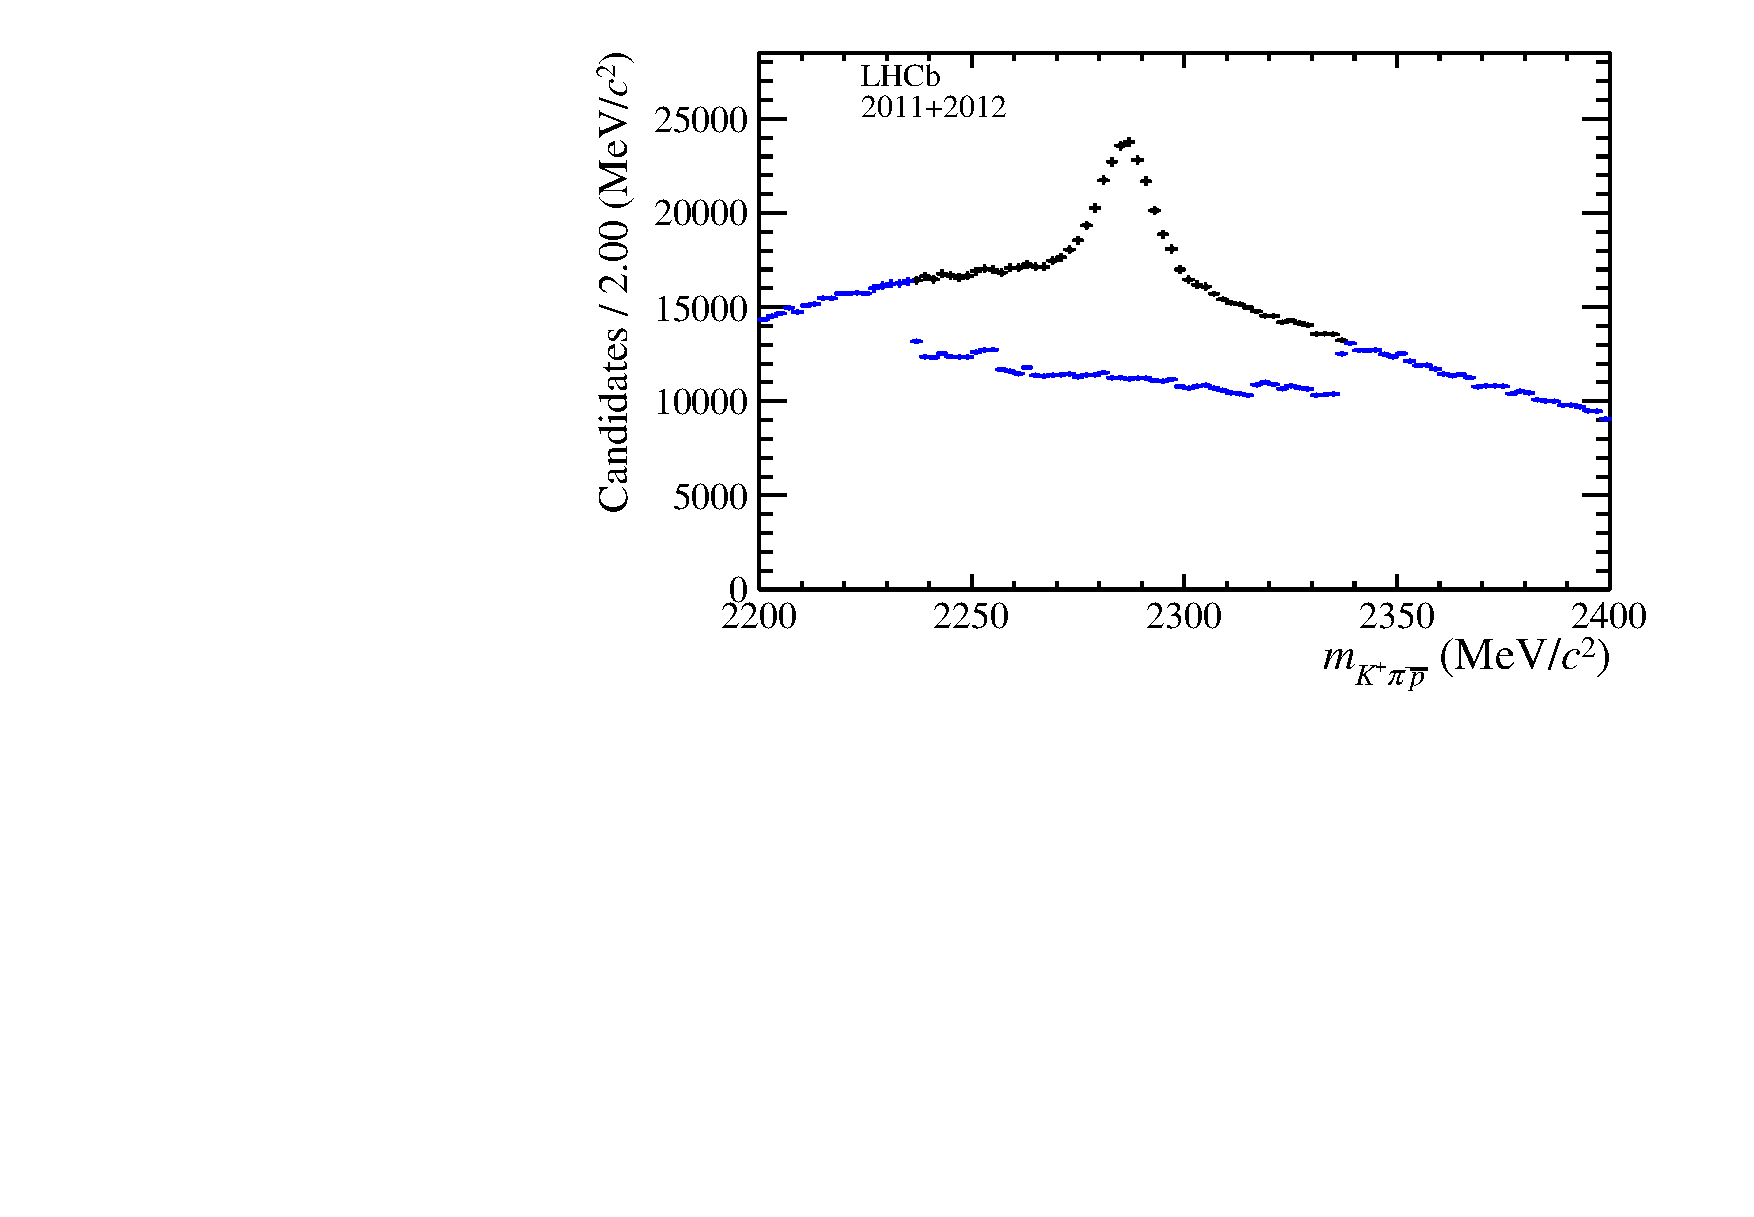
\includegraphics[width=0.45\textwidth]{02Selection/figs/LcHypo2.pdf}
	\end{center}
        \vspace{-2mm}
	\caption{Distributions of the invariant mass of the $\Kpm\pimp p^\mp$ combinations
	where each of the two daughter pions of the $\Dmp$ meson candidate is assigned in turn the proton mass. The
	distribution is given without (black) and with (blue) the $\Lambda_c^{\mp}$
	veto described in the text. On the left (right) the proton mass hypothesis is
	applied to the pion with the lower (higher) $\pt$.}
	\label{fig:lambdaveto}
\end{figure}

In the same way as protons may be misidentified as pions, it is possible for kaons
to be misidentified as pions. Such a mis-identification would lead to background
contributions from $\Bs\to\Dsm\left(\to\Kp\Km\pim\right)\pip$. To check for
these contributions, the kaon mass hypothesis is applied in turn to each of the two pions
from the $\Dmp$ final state. The invariant mass of the resulting
$\Kpm\Kmp\pimp$ system is recalculated and plotted for two different ranges of
the $\Bs$ mass: the first range, from \SIrange{5330}{5400}{\MeVcc}, covers the
signal region of the $\Bs$ meson as possible background
contribution. The
second range, from \SIrange{5500}{5700}{\MeVcc} is the upper mass \emph{sideband} for
this possible background contamination. As can be seen in Fig.~\ref{fig:Dsveto}
the distribution in the $\Bs$ signal region does not
show any significant peaking structure compared to that in the upper $\Bs$ mass sideband
region. The visible differences are expected as the distributions arise from
different kinematic ranges.
%
\begin{figure}[t]
	\begin{center}
		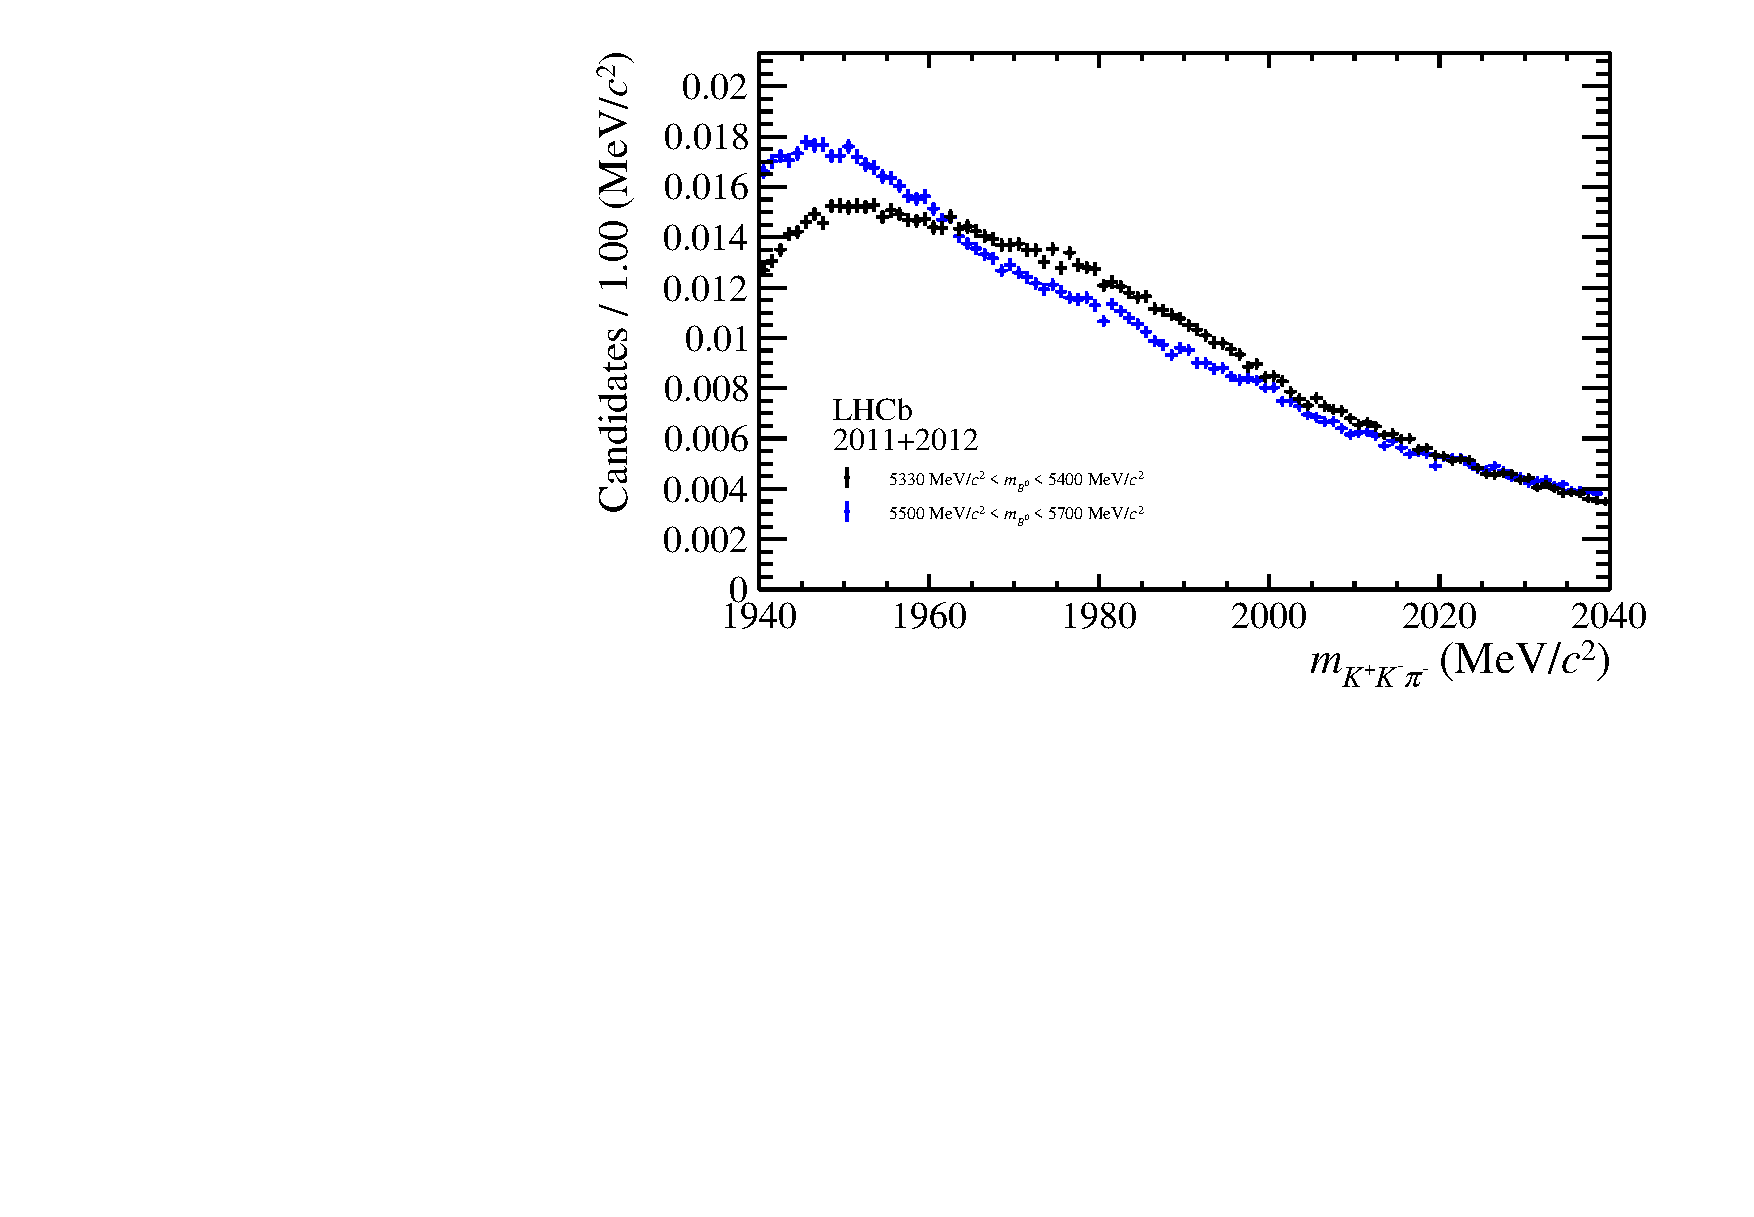
\includegraphics[width=0.45\textwidth]{02Selection/figs/DsHypo1.pdf}
		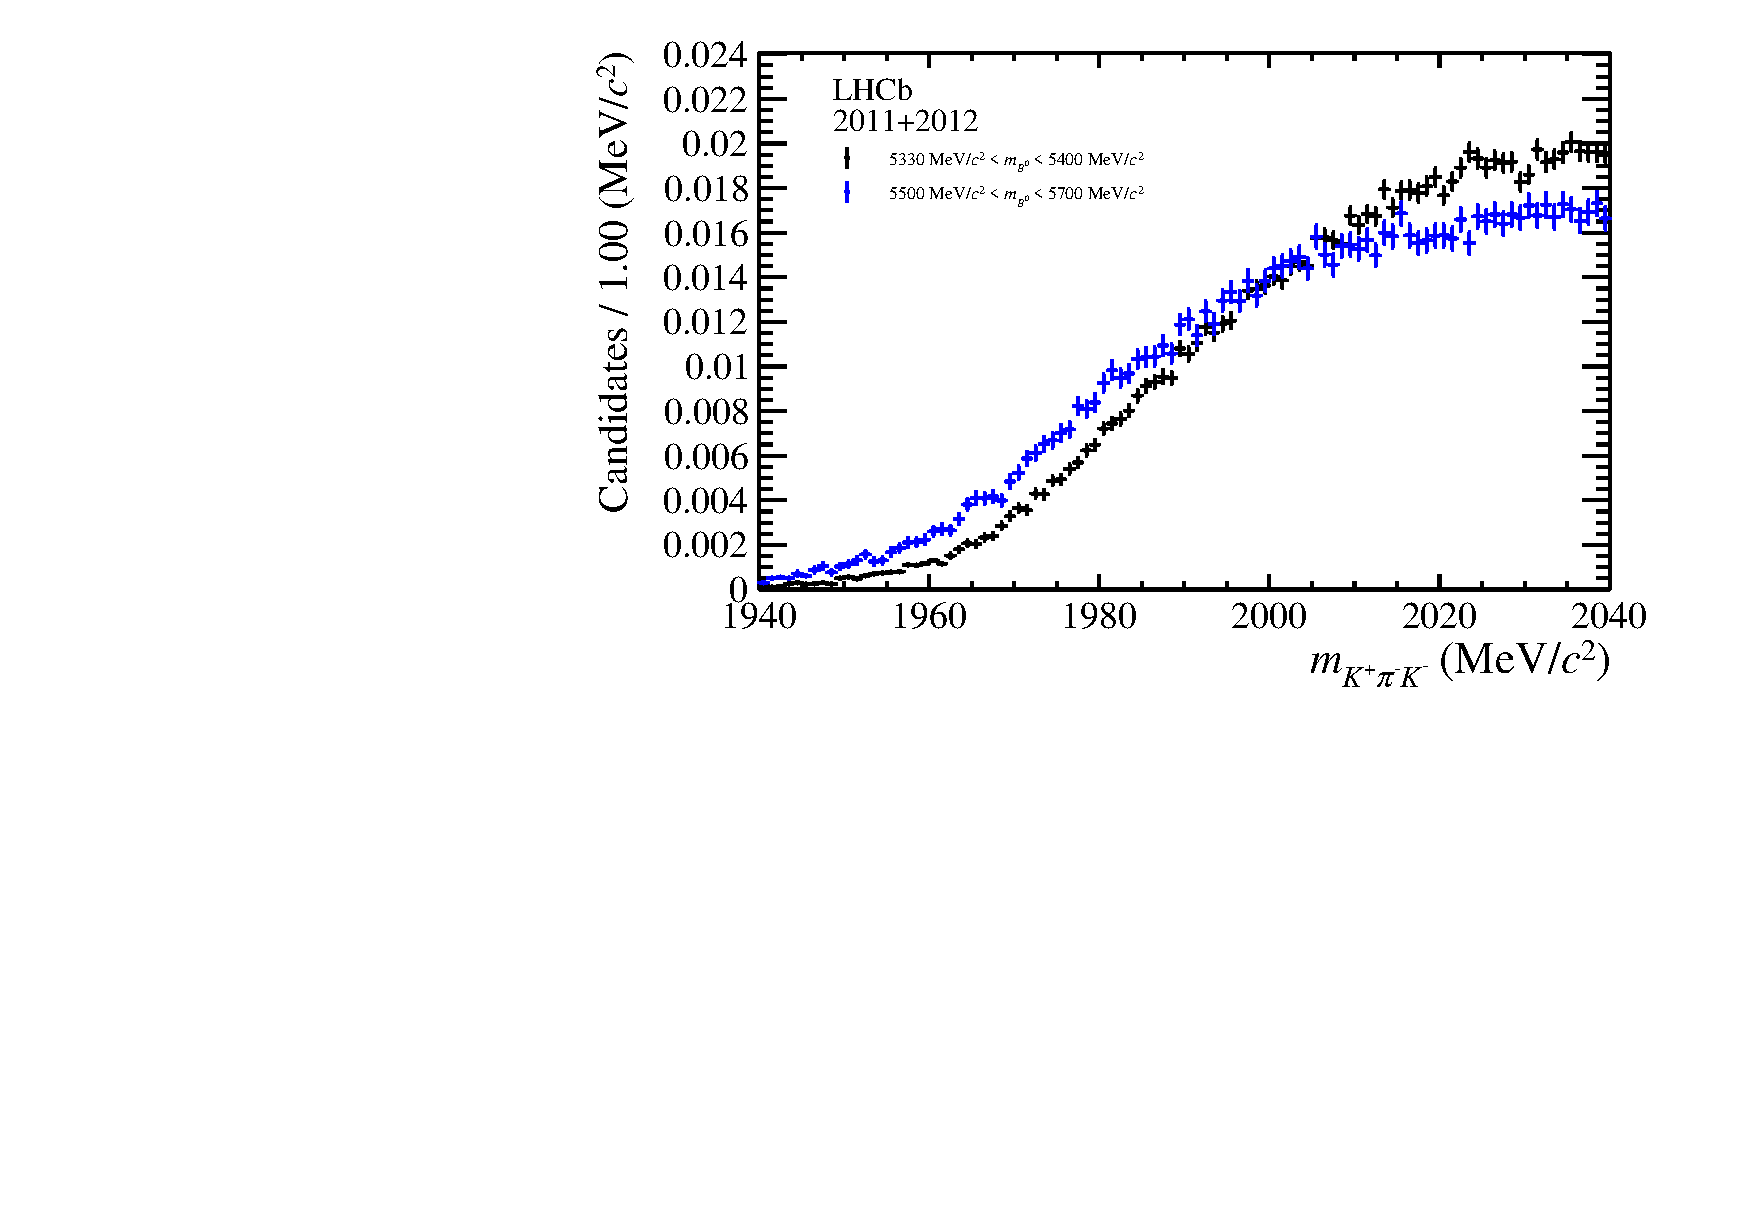
\includegraphics[width=0.45\textwidth]{02Selection/figs/DsHypo2.pdf}
	\end{center}
        \vspace{-2mm}
	\caption{Distributions of the invariant mass of the $\Kpm\Kmp\pimp$ combinations where each of the two 
	daughter pion of the $\Dmp$ meson candidate is assigned in turn the kaon mass. The
	distributions are given in the $\Bs$ meson mass range from
	\SIrange{5330}{5400}{\MeVcc} (black) and in the  $\Bs$ meson mass range
	from \SIrange{5500}{5700}{\MeVcc} (blue) after applying the $\Lambda_c^{\mp}$ veto.
	On the left (right) the kaon mass hypothesis is applied to the pion with the lower (higher) $\pt$.}
	\label{fig:Dsveto}
\end{figure}
%
To double check for possible resonant contributions from a kaon mis-identification, the decay
of the $\Dmp$ meson after applying the kaon mass hypothesis is investigated.
Possible resonant decays of the $\D$ meson can take place via a \Kstar~or $\phi$
resonance. These resonances would be visible in the $\kaon\pion$ and
$\kaon\kaon$ invariant mass distributions, which are plotted for the same two
ranges in Fig.~\ref{fig:KstarAndPhi}. As the distributions in the signal and
background ranges look compatible, the $\Dsmp$ contamination is
negligible and no veto is applied.
%
\begin{figure}[t]
	\begin{center}
		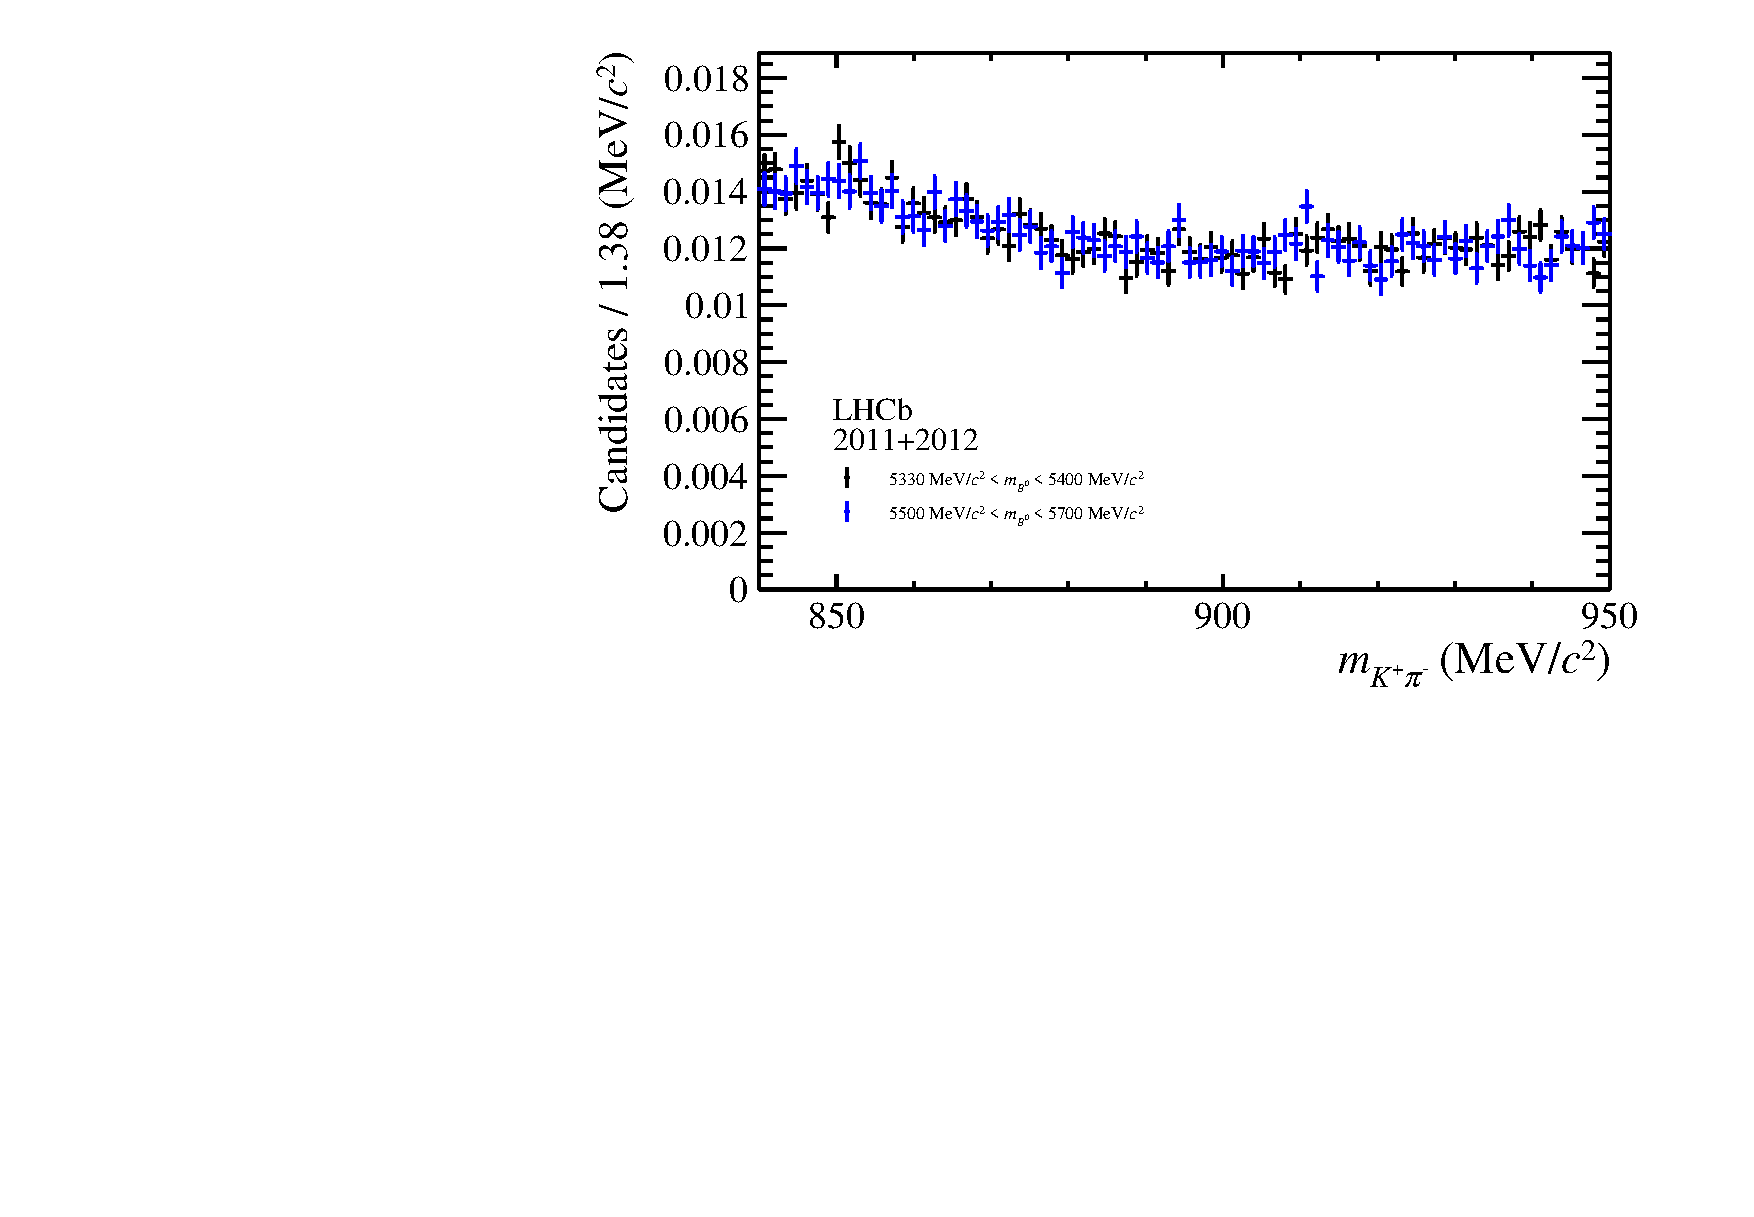
\includegraphics[width=0.45\textwidth]{02Selection/figs/KstarHypo1.pdf}
		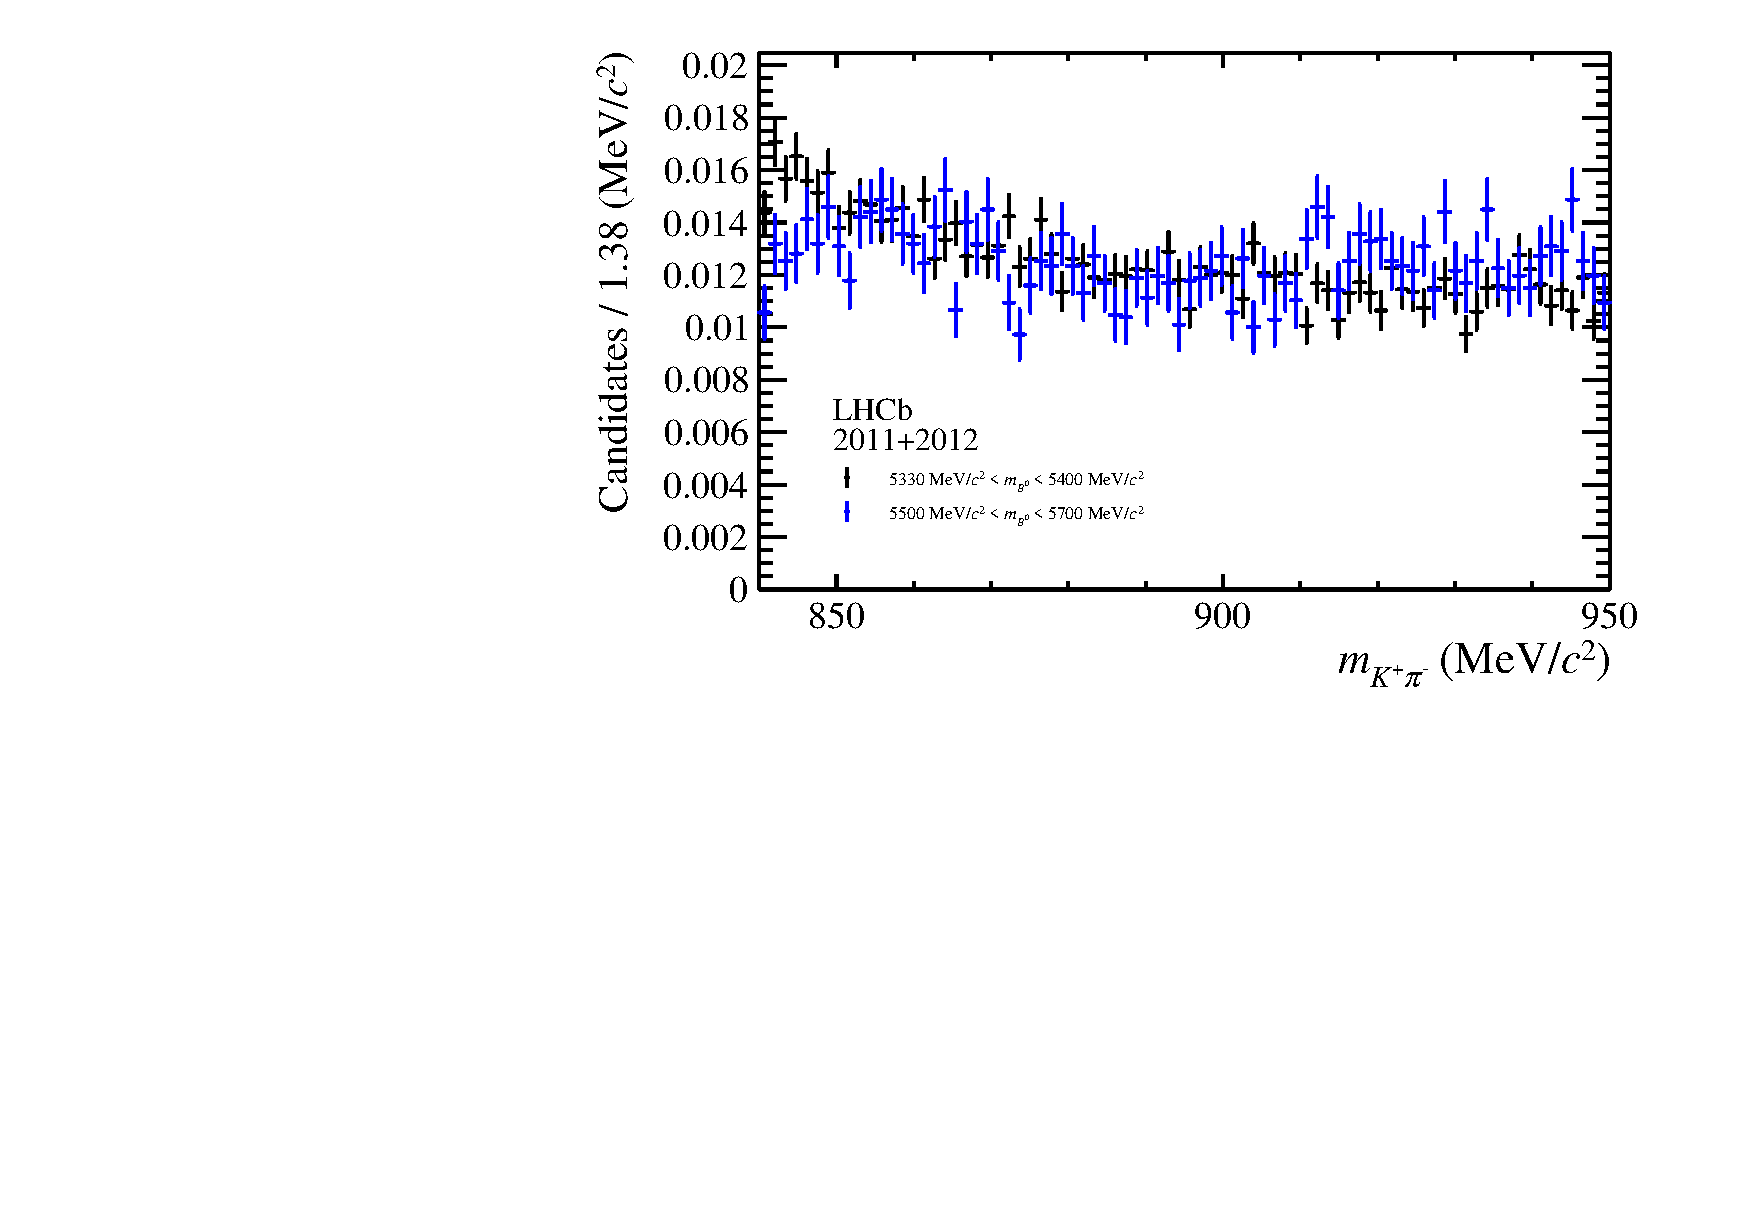
\includegraphics[width=0.45\textwidth]{02Selection/figs/KstarHypo2.pdf}\\
		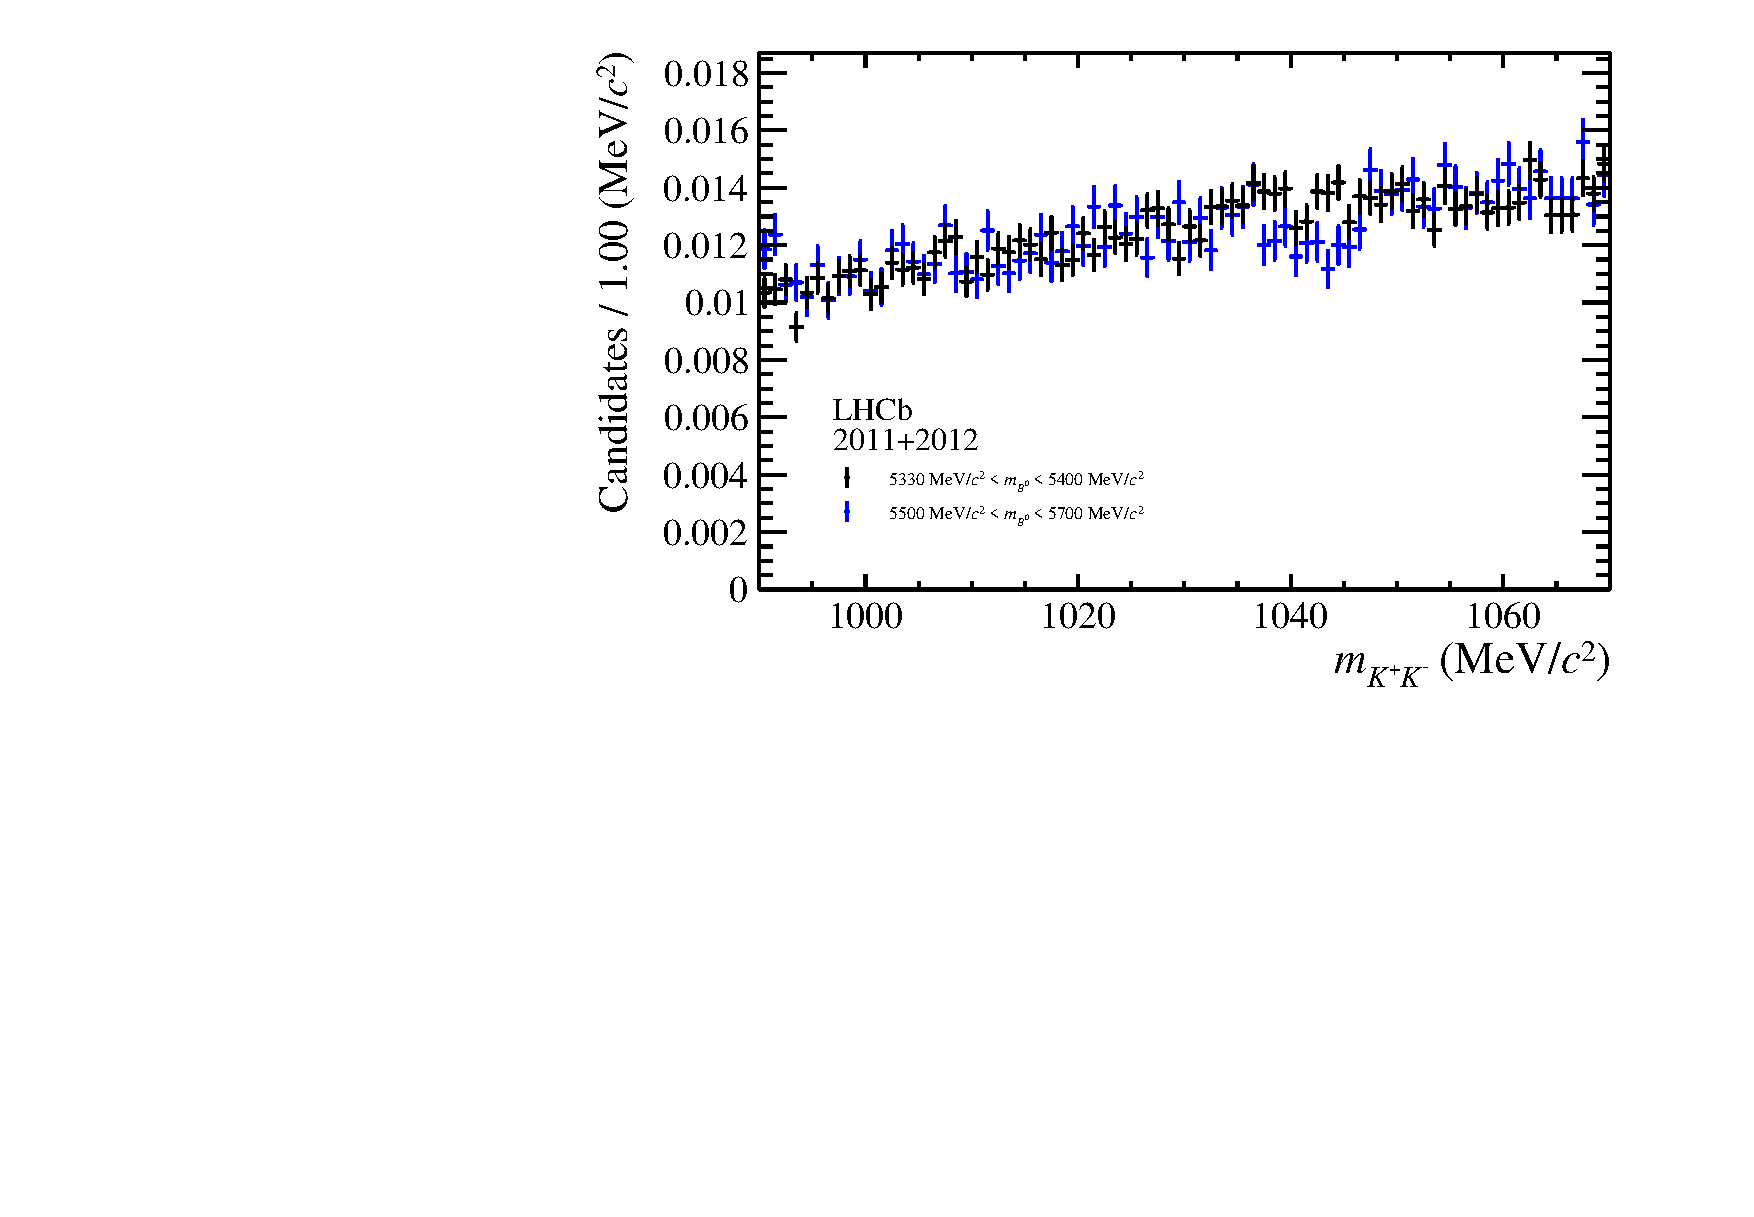
\includegraphics[width=0.45\textwidth]{02Selection/figs/PhiHypo1.pdf}
		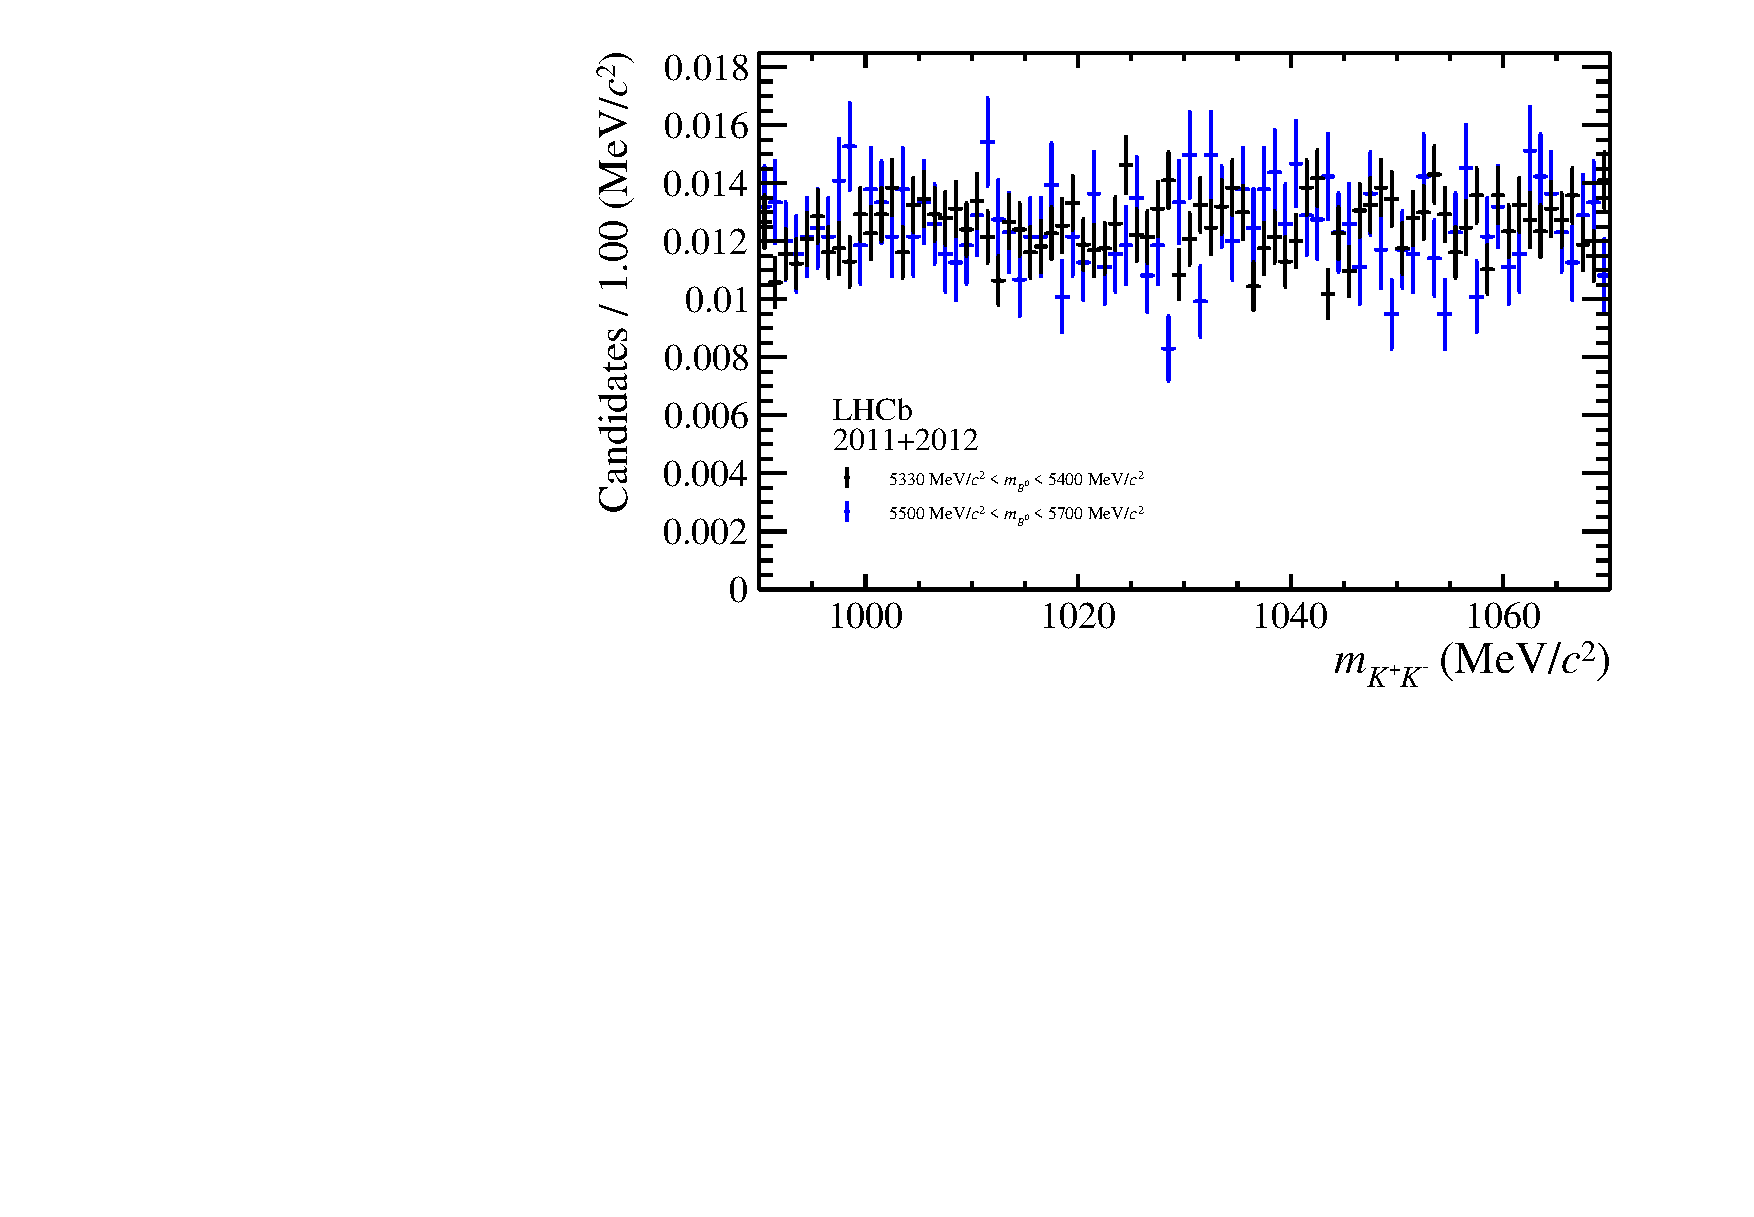
\includegraphics[width=0.45\textwidth]{02Selection/figs/PhiHypo2.pdf}
	\end{center}
        \vspace{-2mm}
	\caption{Distributions of the invariant mass of the $\Kmp\pipm$ combination (top) and
	the $\Kmp\Kpm$ combination (bottom), where each of the two daughter pion of the
	$\Dmp$ meson candidate is assigned in turn the kaon mass. The distributions are shown in the $\Bs$ meson mass range of $[5330,5400]~\mevcc$
	(black) and $[5500,5700]~\mevcc$ (blue) as described in the text.
	Additionally, the $\Dsmp$ mass is required to be in
	$[1940,2040]~\mevcc$. On the left (right) the kaon mass
	hypothesis is applied to the pion with the lower (higher) $\pt$.}
	\label{fig:KstarAndPhi}
\end{figure}
%
In the same way as for the $\Dmp$ meson daughters, it is also possible that the
bachelor pion candidate is actually a misidentified kaon. This mis-identification could lead
to background contributions of
\mbox{$\Bz\to\Dz\left(\to\Kpm\pimp\right)\pimp\Kpm$}. A similar background, \mbox{$\Bz\to\Dz\left(\to\Kpm\pimp\right)\Kmp\pipm$},
could arise if one $\Dmp$ meson daughter pion is misidentified as a
kaon and combined with the bachelor pion. To check for this contribution, the
kaon mass hypothesis is applied to the bachelor pion and the $\D$ meson daughter
pions, and the invariant mass distributions for the four possible $\kaon\pion$
systems are plotted after applying the MVA classifier described in Sec.~\ref{sec:mvaclassifier} (Fig.~\ref{fig:D0veto}). As the
distributions show no significant peaking structures, this
contribution is neglected and no specific
cuts are applied.
%
\begin{figure}[t]
	\begin{center}
		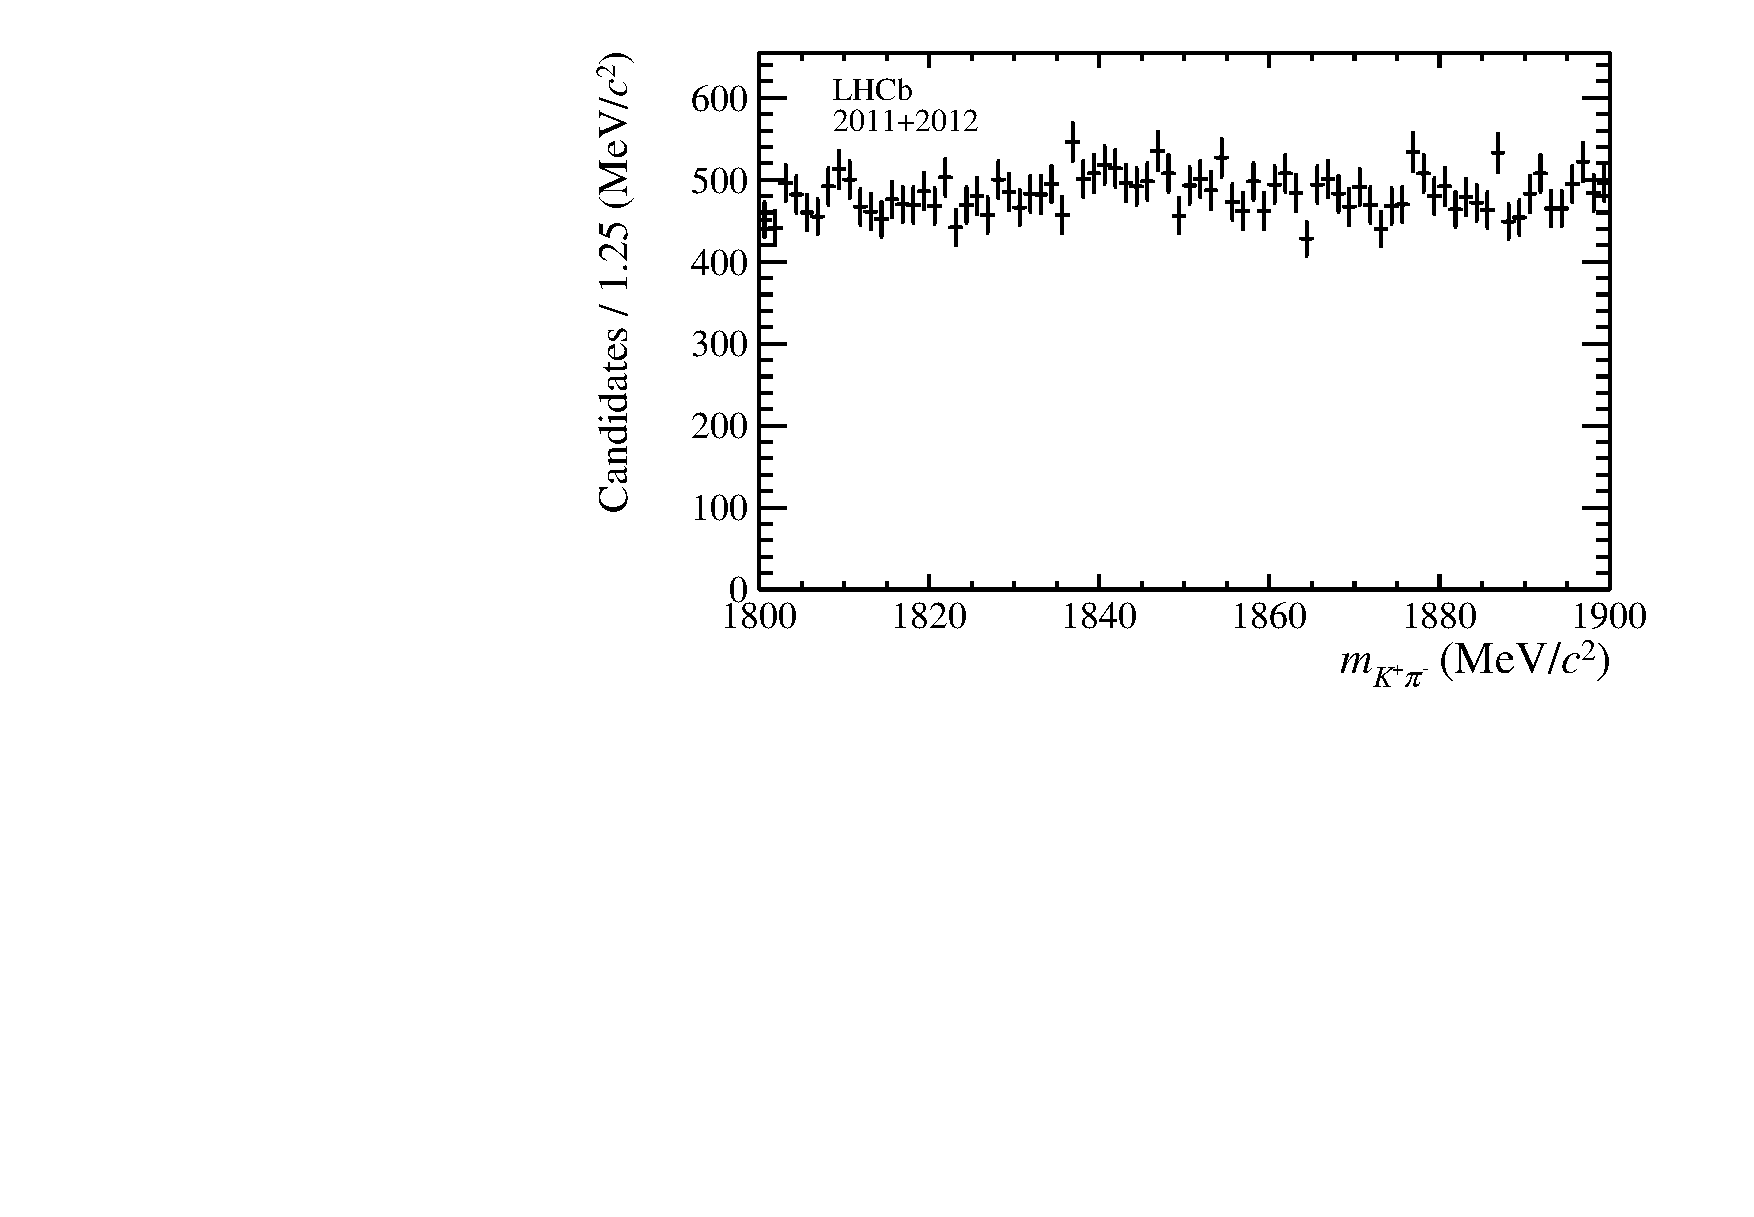
\includegraphics[width=0.45\textwidth]{02Selection/figs/D0Hypo1.pdf}
		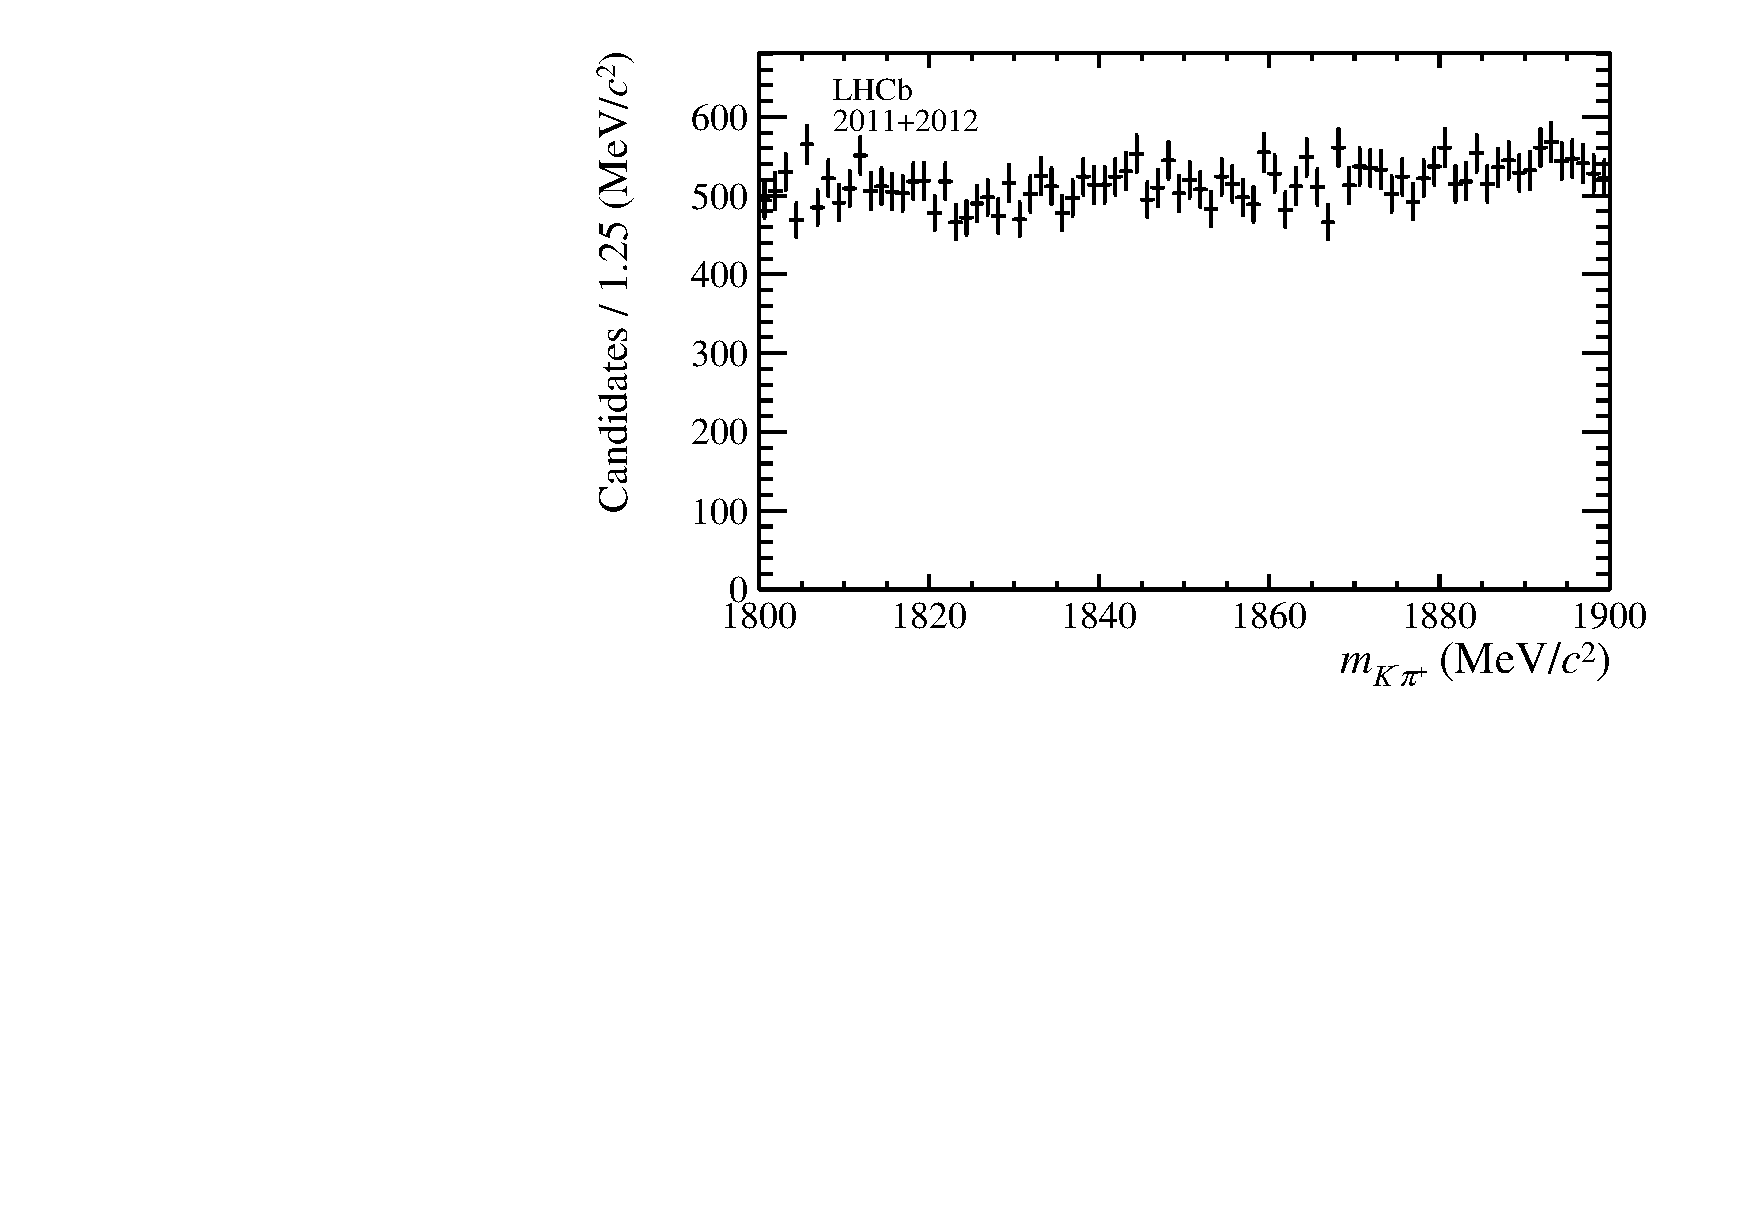
\includegraphics[width=0.45\textwidth]{02Selection/figs/D0Hypo2.pdf}\\
		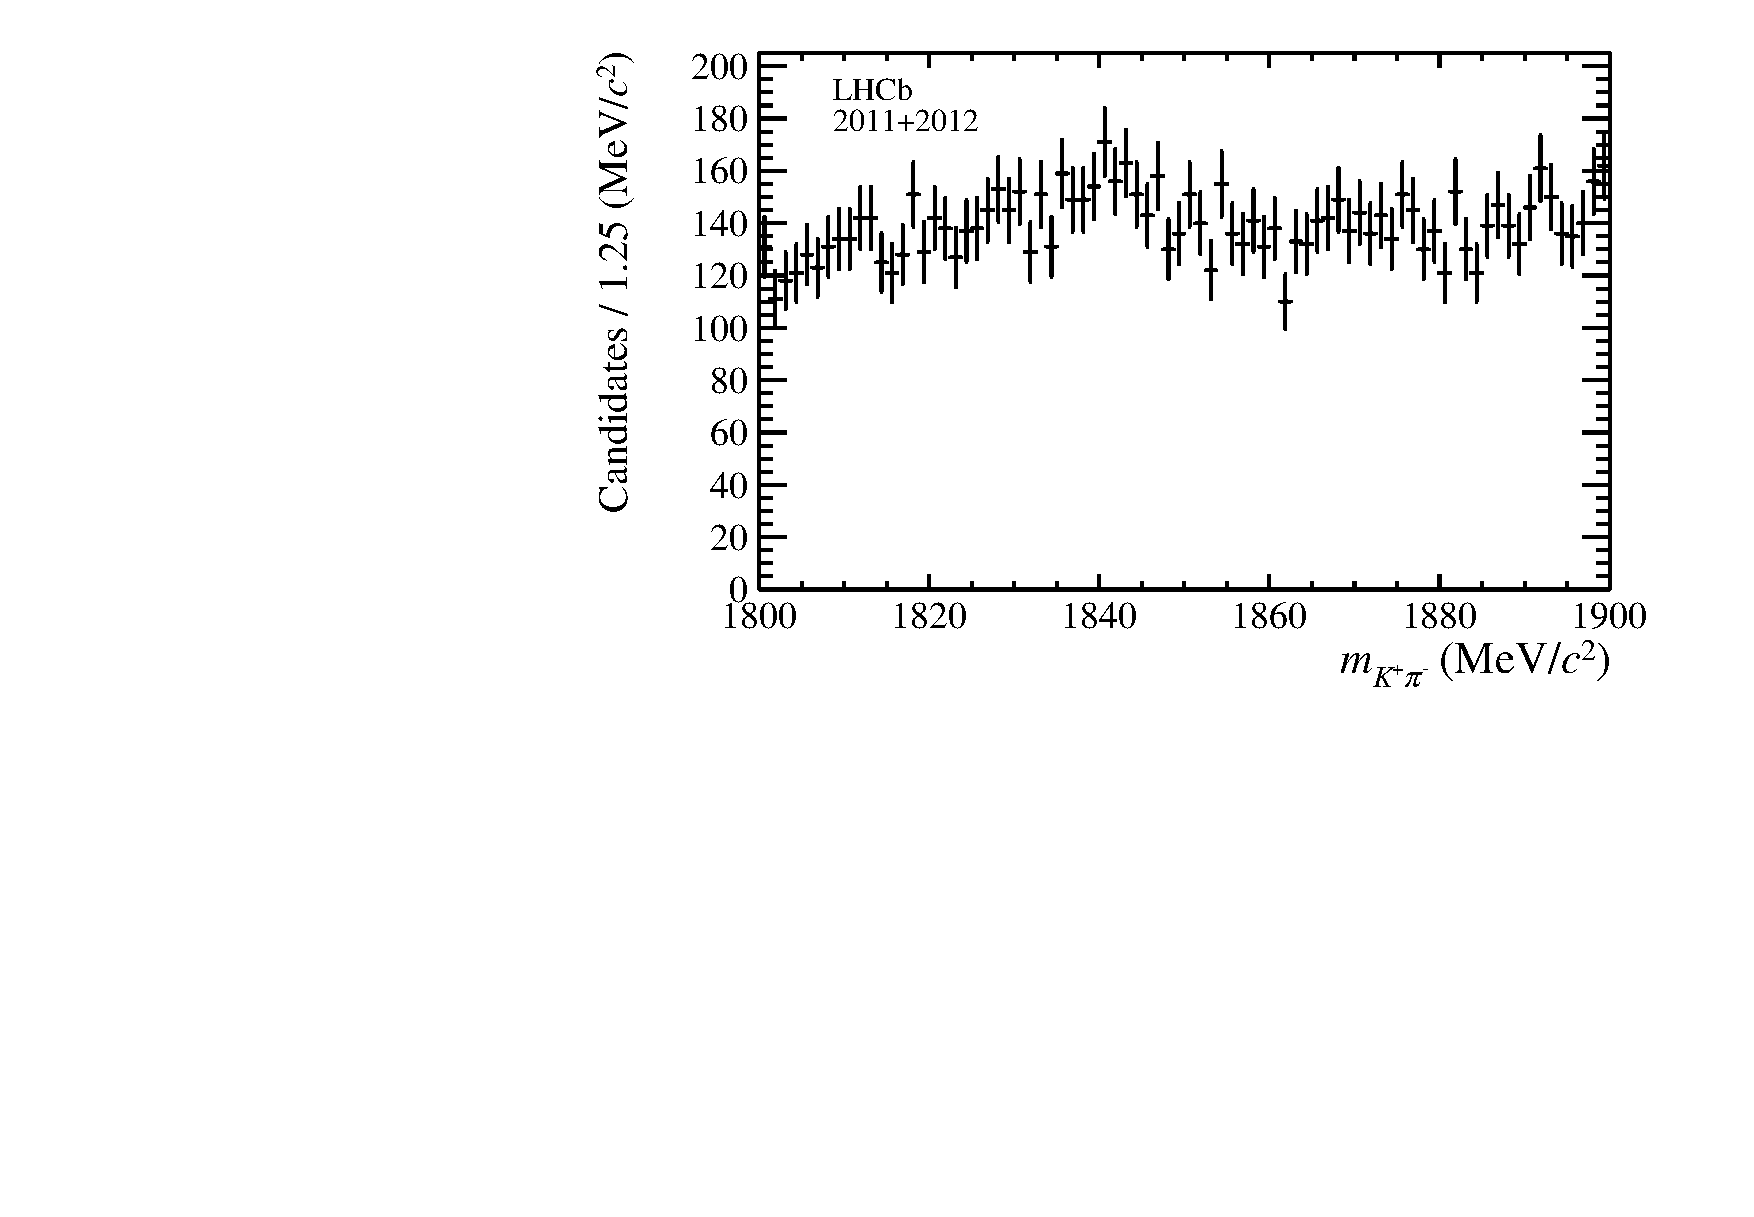
\includegraphics[width=0.45\textwidth]{02Selection/figs/D0Hypo3.pdf}
		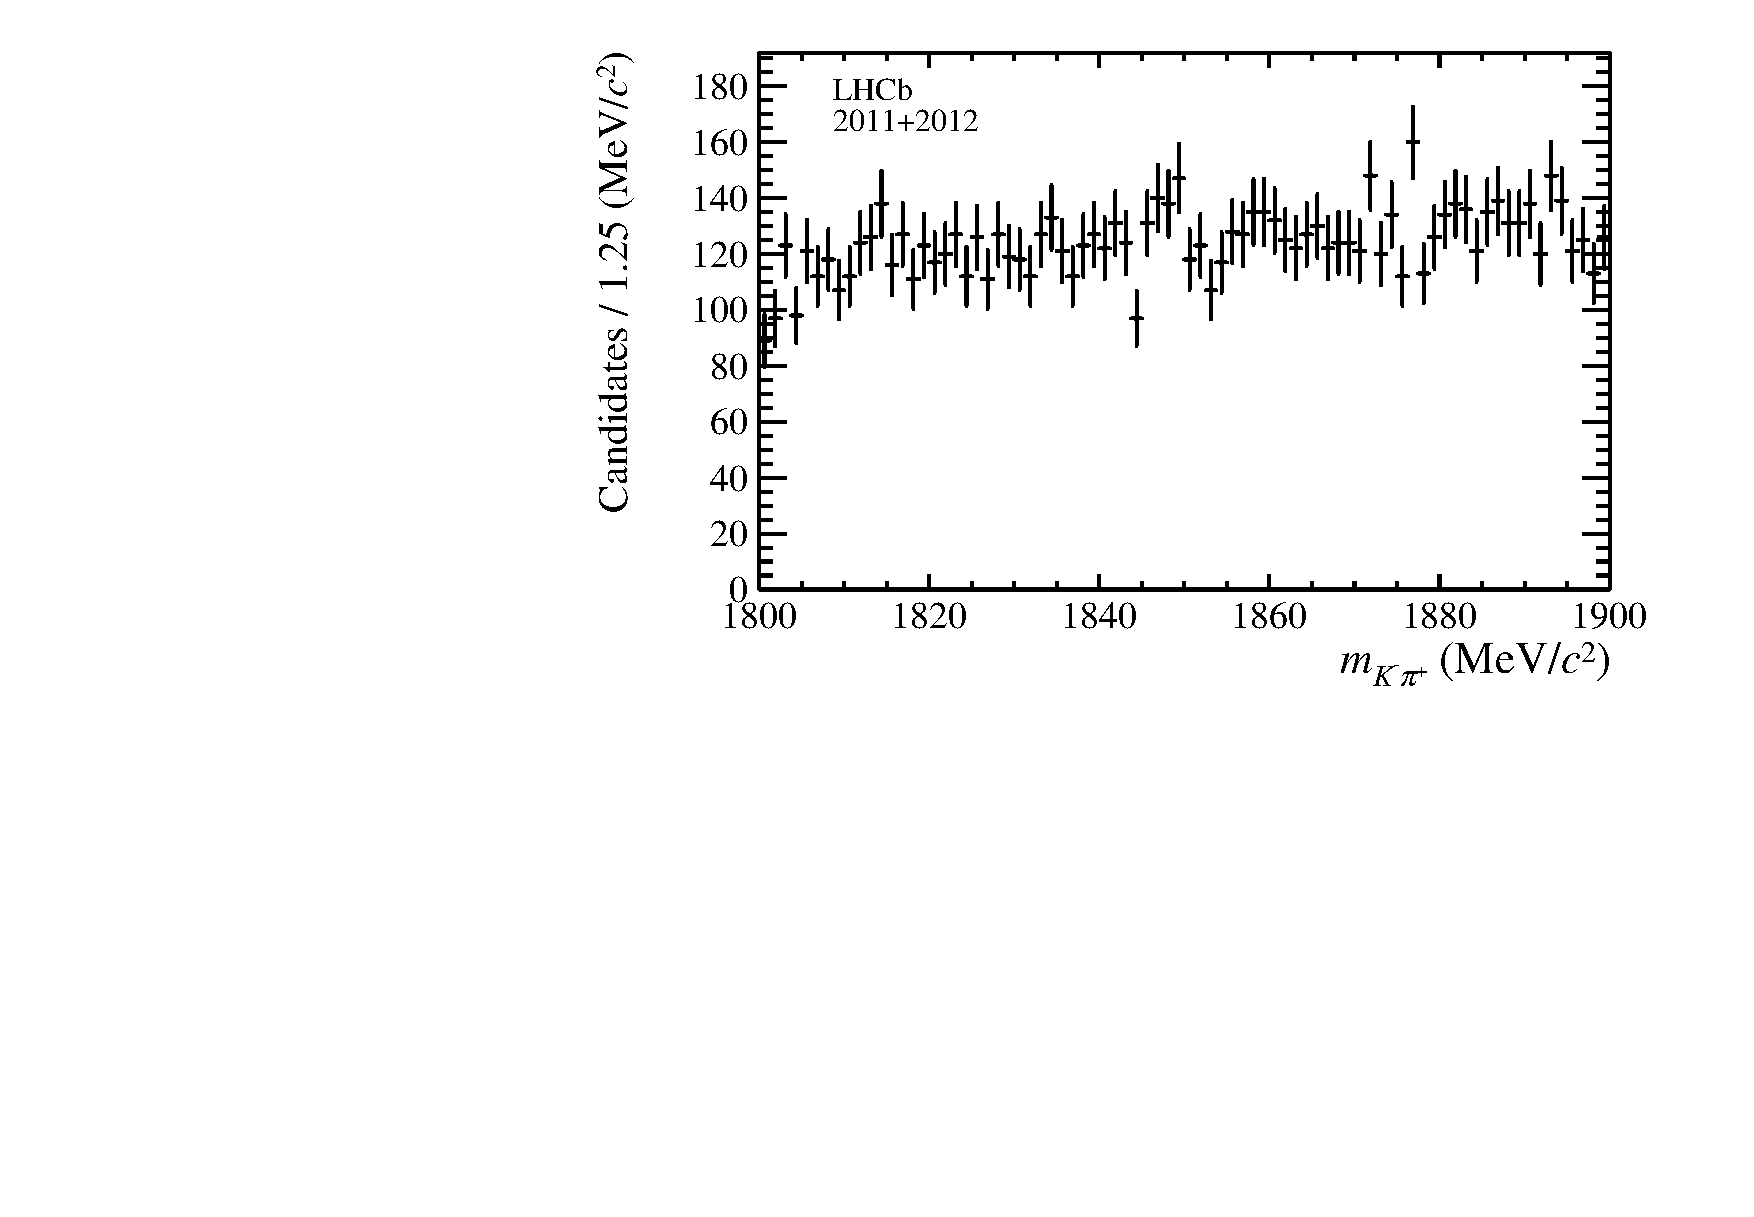
\includegraphics[width=0.45\textwidth]{02Selection/figs/D0Hypo4.pdf}
	\end{center}
        \vspace{-2mm}
	\caption{Distributions of the invariant mass of the four possible $\Kmp\pipm$
	combinations. In the top (bottom) plots the bachelor pion is combined with the pion from the $\Dmp$ meson with lower (higher) $\pt$. 
	In the left (right) plots the
	kaon mass hypothesis is applied to the bachelor pion (pions from the $\Dmp$ meson).}
	\label{fig:D0veto}
\end{figure}


%-------------------------------------------------------------------------------
\subsection{Wrongly associated primary vertices}
\label{sec:WrongPVs}

Given an average number of total $pp$ interactions per bunch crossing of
$\nu=\num{2.5}$, a large fraction of events have more than one reconstructed PV.
The PV to which the $\Bz$ candidate has the smallest IP$\chi^2$ (\emph{best} PV) is chosen as the $\Bz$ production vertex.

In events where the association of the $\Bz$ candidate to its best PV
is wrong, the reconstructed decay time of this candidate will be incorrect. These wrongly
associated candidates cause a large tail in
the decay time distribution, which can be clearly observed in signal MC where the
true decay time is known: giving each candidate a weight equal to $e^{t/\tau}$, where $\tau$ is the
true lifetime, leads to an excess of candidates at high decay times.
%
\begin{figure}[t]
	\begin{center}
		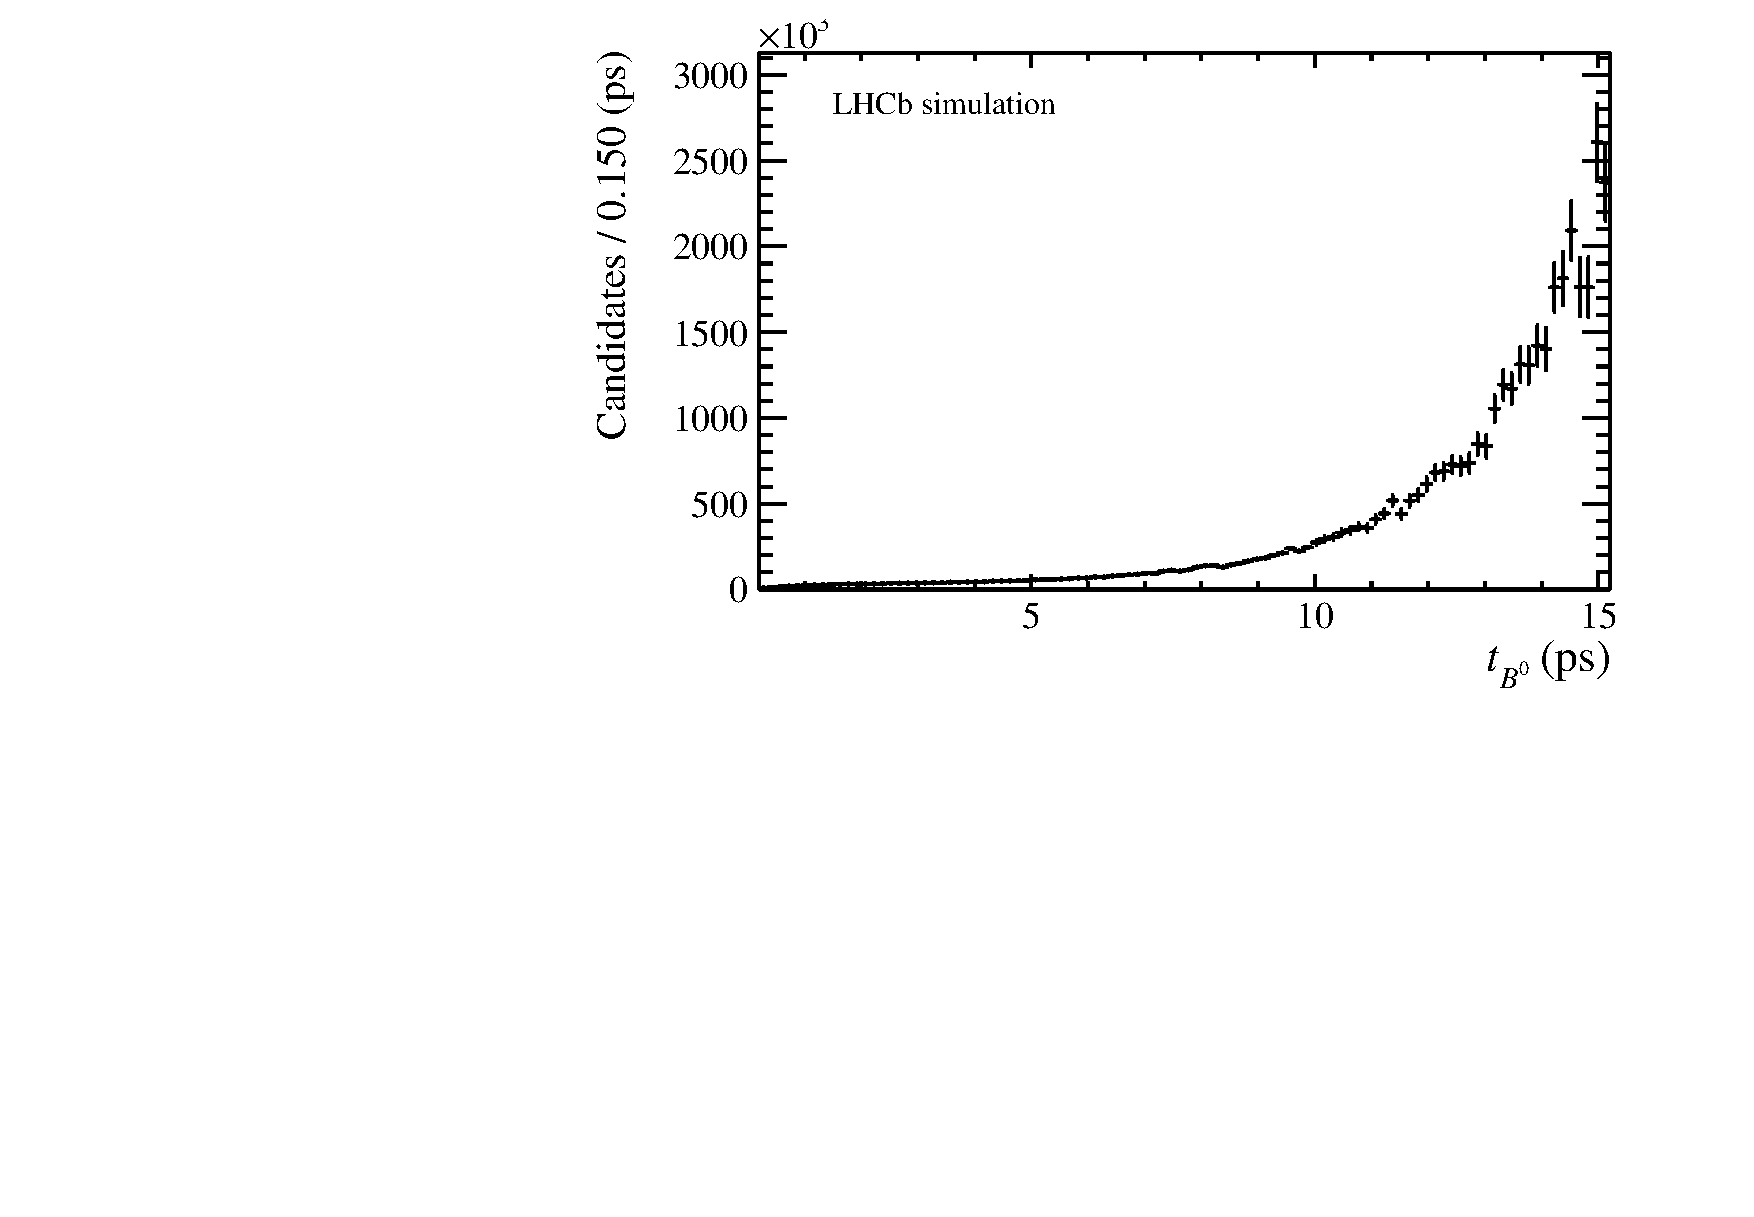
\includegraphics[width=0.45\textwidth]{02Selection/figs/WrongPVs-weightedBad.pdf}
		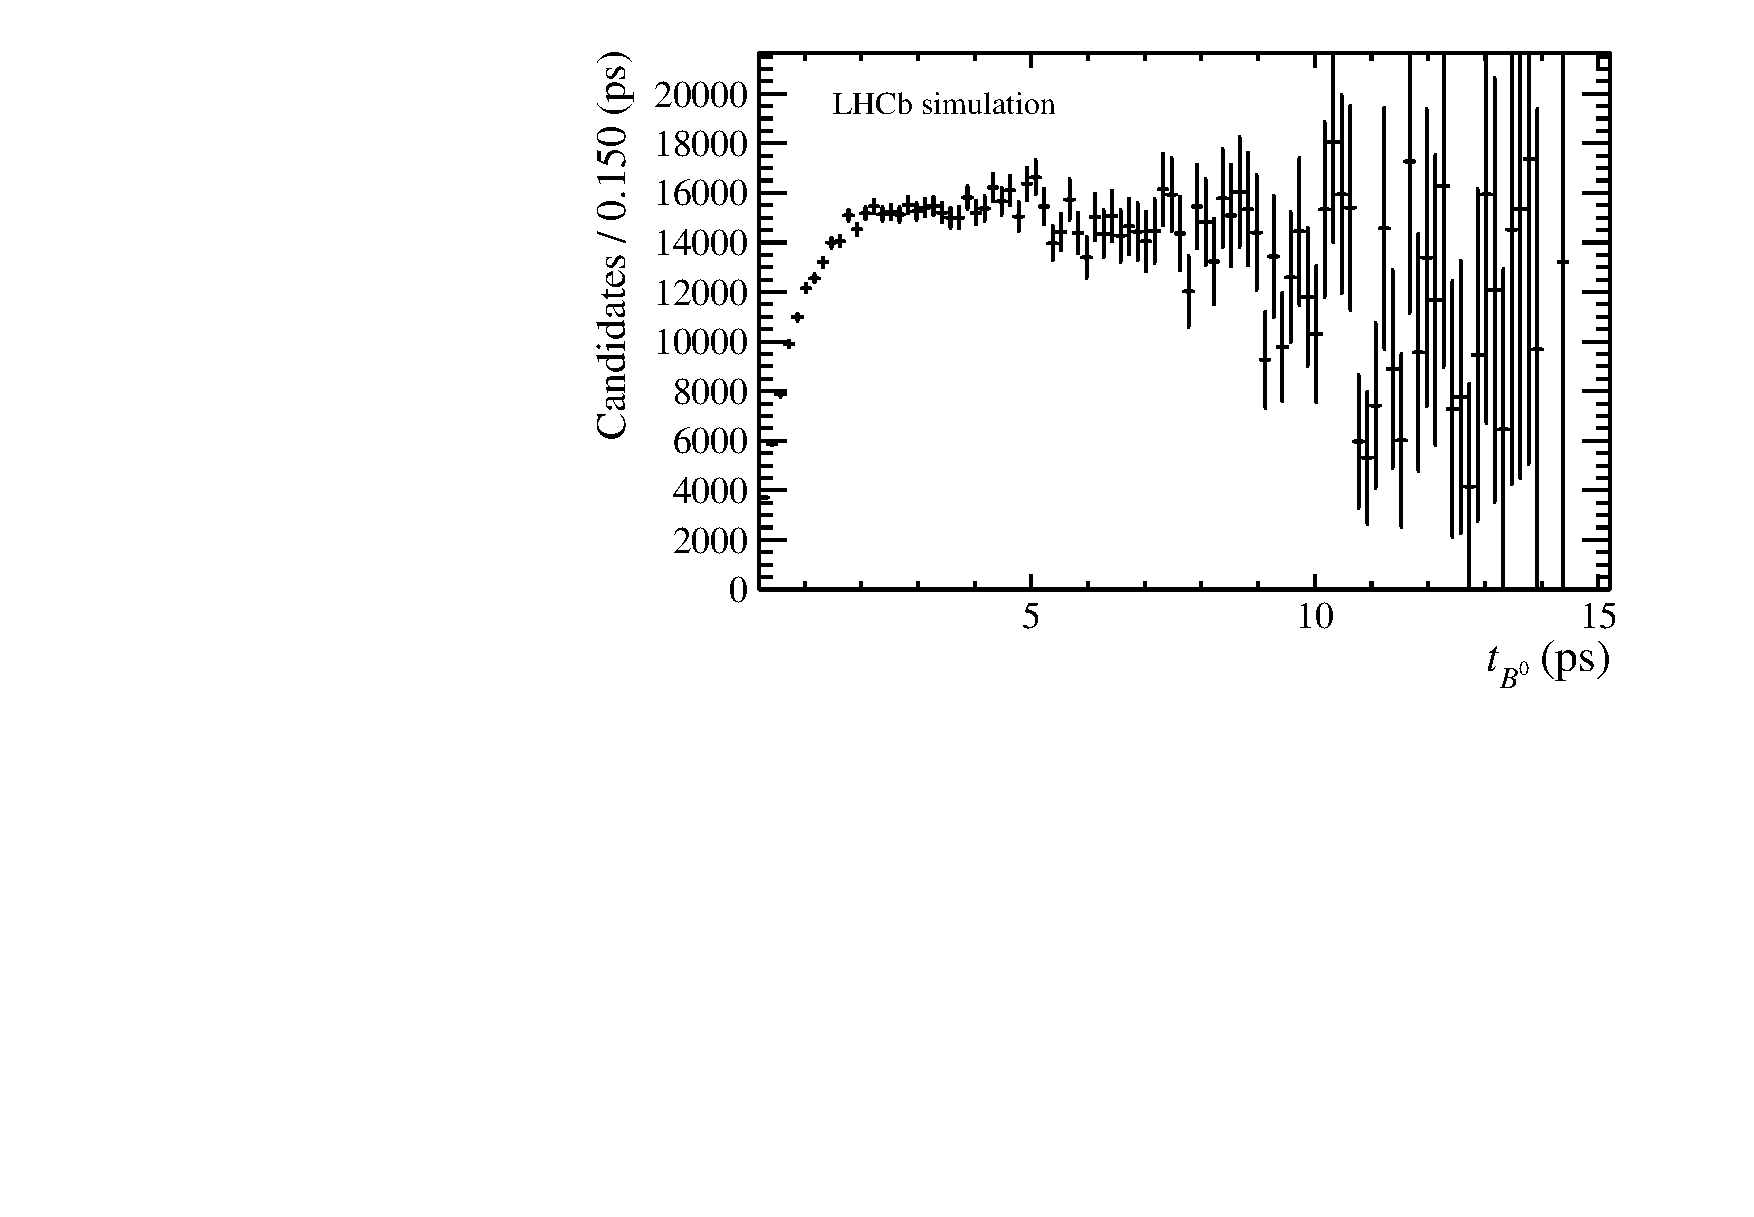
\includegraphics[width=0.45\textwidth]{02Selection/figs/WrongPVs-weightedGoodMC.pdf}
	\end{center}
        \vspace{-2mm}
	\caption{Left: decay time distribution of signal MC events weighted with $e^{t/\tau}$, where $\tau$ is
	the true lifetime. At high decay times an excess of candidates can be
	observed. Right: same distribution after requiring that the
	absolute difference between the best PV $z$ position and the true PV $z$ position is within
	$5$ times the best PV $z$ position uncertainty. As the excess of candidates at high decay
	times vanishes (from left to right), it is concluded that this excess is due to candidates
	wrongly associated to their PV.}
	\label{fig:wrongPVs_MC}
\end{figure}
%
To remove these incorrect associations in MC, one can compare the
$z$ position of the associated PV with the $z$ position of the true PV and
reject the candidate if the distance between those positions exceeds 5 times its
uncertainty (Fig.~\ref{fig:wrongPVs_MC}). 
In real data, the true PV in unknown, so a selection involving
the $\Bz$ impact parameter $\chi^2_\text{DTF,PV}$ is adopted instead.
If there are multiple PVs in an event, the $\Bz$ candidate is constrained by DTF to originate,
in turn, from each of them; then, the $\chi^2_\text{DTF,PV}$ with respect to all the other
PVs is computed, and the smallest one (called $\mathrm{MinIP}\chi^2$) is considered.
(Fig.~\ref{fig:MinIPCHI2}).
%
\begin{figure}[t]
	\begin{center}
		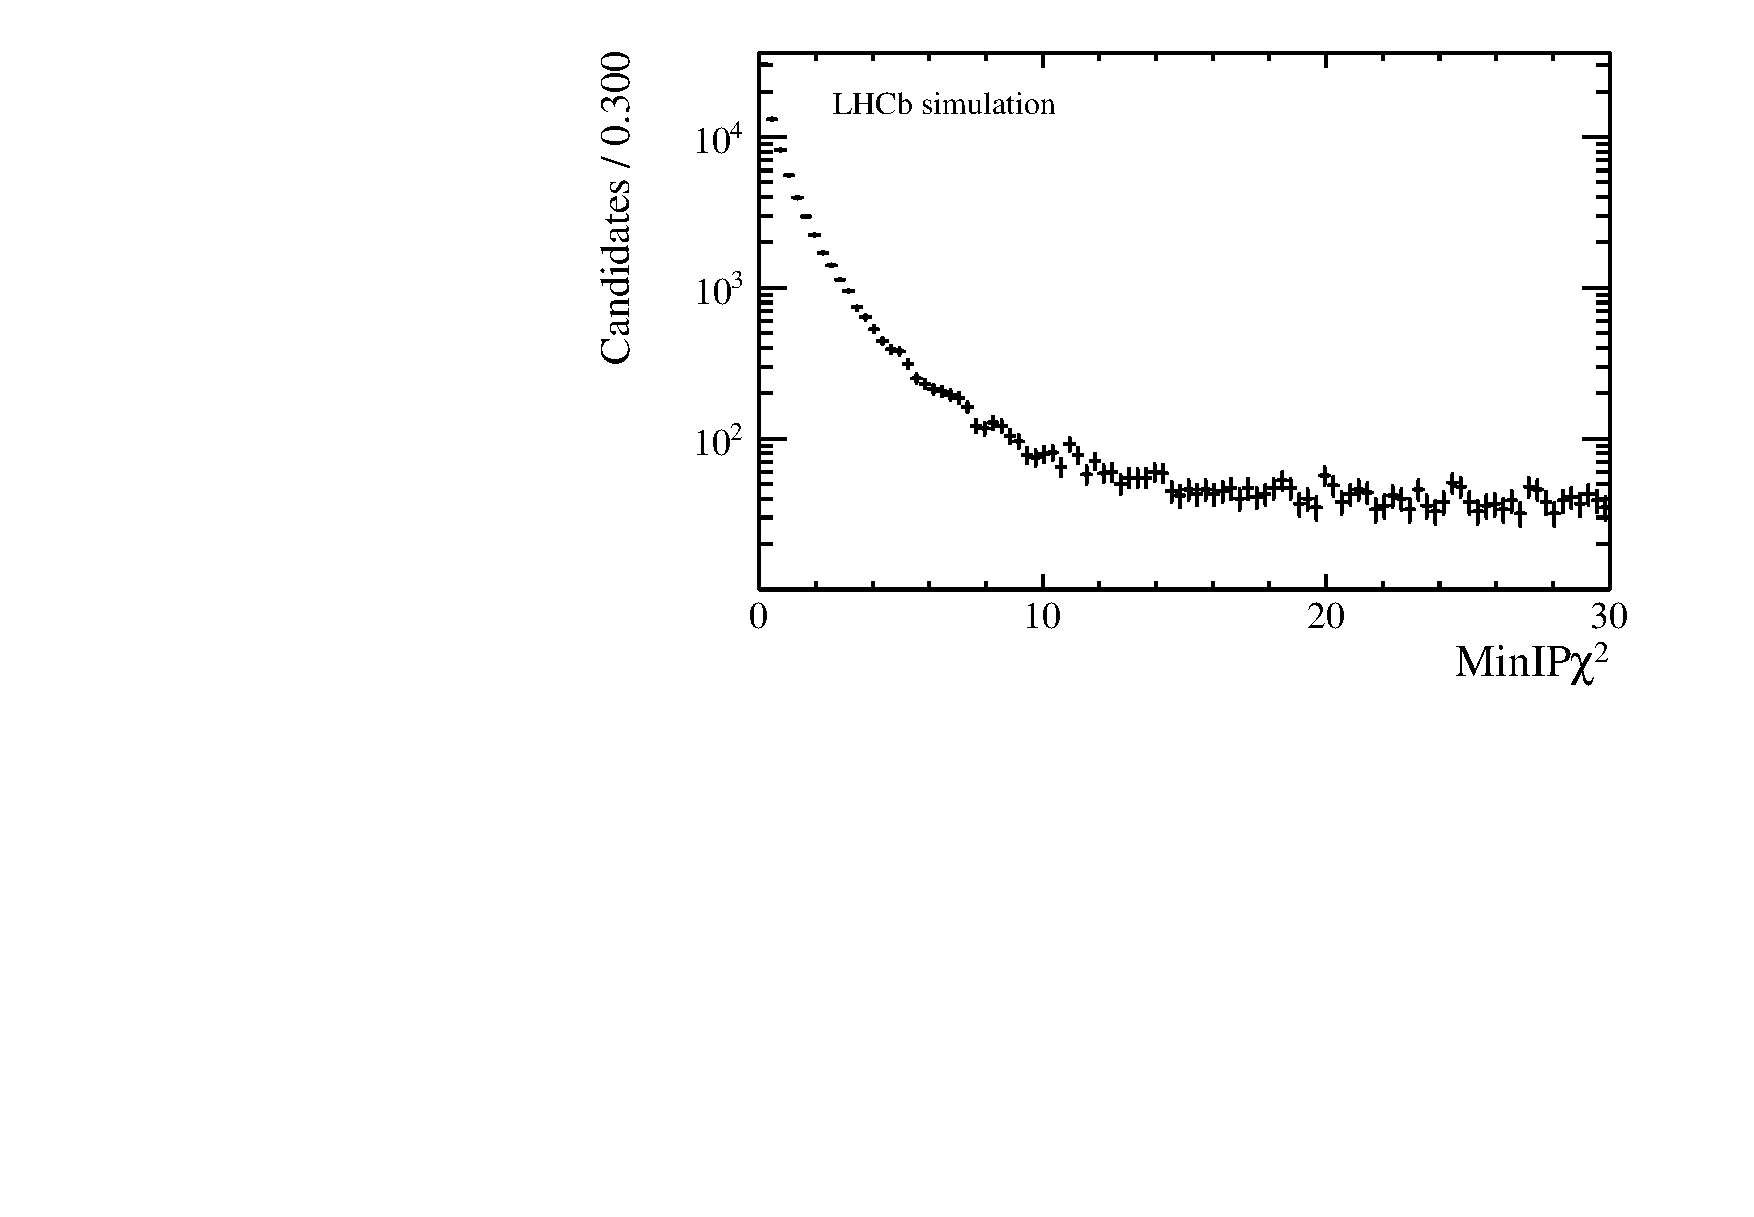
\includegraphics[width=0.45\textwidth]{02Selection/figs/MinIPCHI2.pdf}
		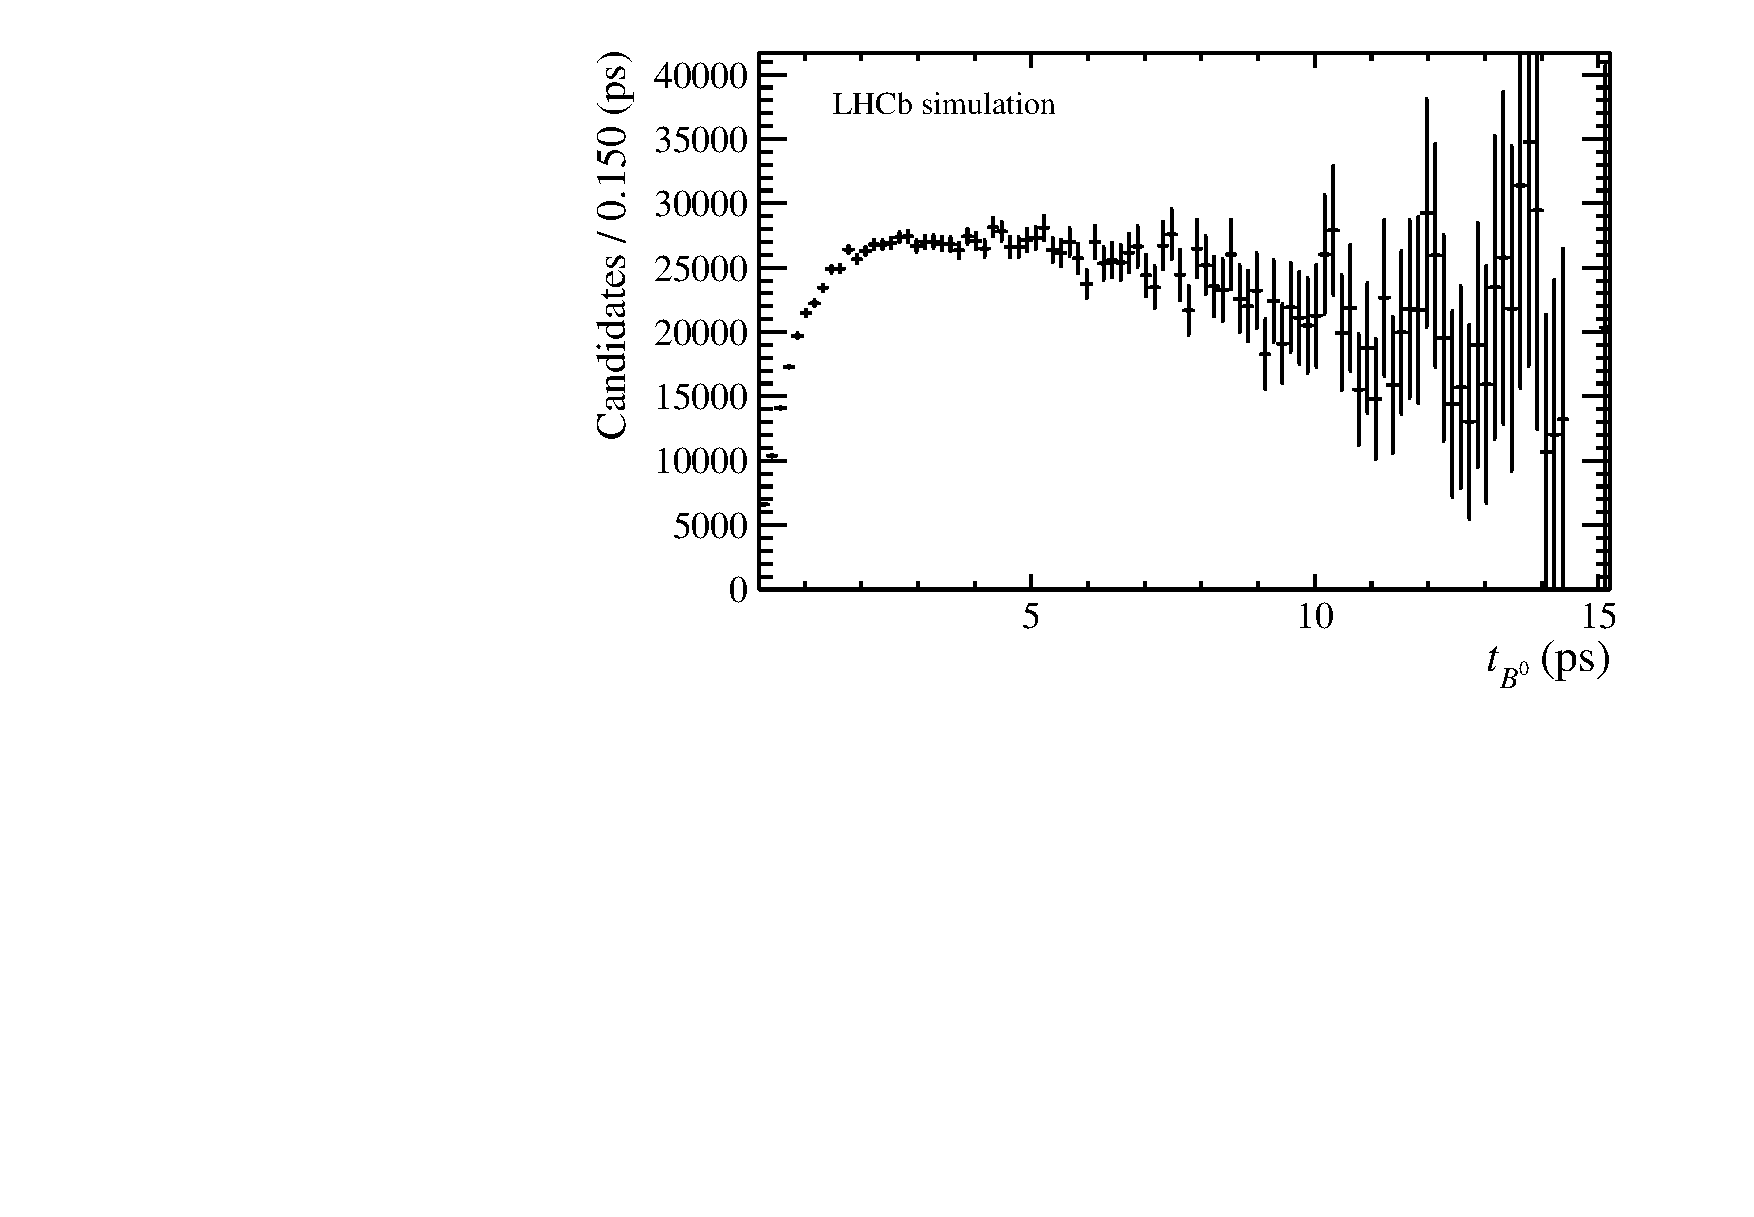
\includegraphics[width=0.45\textwidth]{02Selection/figs/WrongPVs-WeightingGoodData.pdf}
	\end{center}
        \vspace{-2mm}
	\caption{Left: distribution of $\mathrm{MinIP}\chi^2$
	for signal MC events. Right: decay time distribution 
	of signal MC events weighted with $e^{t/\tau}$, where $\tau$ is the true lifetime, 
	after requiring that $\mathrm{MinIP}\chi^2>16.5$.}
	\label{fig:MinIPCHI2}
\end{figure}
For events with only a single PV, $\mathrm{MinIP}\chi^2$ is not defined. The main advantage of this
$\mathrm{MinIP}\chi^2$ variable is that all PVs are treated equally, without any biasing choice. 
The cut on $\mathrm{MinIP}\chi^2$ is optimised to retain \SI{98}{\%} of the truth-matched signal candidates in MC.
The optimal requirement is then found at
$\mathrm{MinIP}\chi^2>\num{16.5}$. A plot showing the signal MC weighted decay time
distribution after applying this cut is given in Fig.~\ref{fig:MinIPCHI2}.

%===============================================================================
\subsection{Development of an MVA classifier}
\label{sec:mvaclassifier}

The combinatorial background, consisting of candidates created from 
random combinations of tracks, is rejected by using a Boosted Decision Tree
(BDT) classifier~\cite{Breiman, Roe}. The signal input to the training stage consists of signal
MC candidates simulated under $\num{2012}$ data-taking conditions, while the upper mass sideband above
$\SI{5500}{\MeVcc}$ from the $\num{2012}$ data sample is used as template for the
combinatorial background. The BDT is trained on one half of these samples, the
other half being used to test its performance. Before the BDT training,
all previous selection steps (the cut-based preselection, the mass vetoes and the wrongly
associated PV veto) are applied. To reduce the number of input features, the ones 
with a correlation larger than $\SI{97}{\percent}$ with any other feature are removed.
The $\num{16}$ final input features are listed in Table~\ref{tab:BDTinput}.
%
\begin{table}[t]
	\centering
	\caption{List of input features used in the training of the BDT.}
	\begin{tabular}{cc}
		\toprule
		\multirow{2}{*}{$\Bz$ candidate}  &  $\cos$ of $\sphericalangle\left[\overrightarrow{\rm Vertex}(\Bz)-\overrightarrow{\rm PV},\vec{p}(\Bz)\right]$ \\
				    &  vertex $\chi^2$\\
				    & DTF $\chi^2$ with best PV constraint \\
		\midrule
		\multirow{7}{*}{$\Dmp$ candidate} & IP$\chi^2$ w.r.t. $\Bz$ vertex\\
				  & IP$\chi^2$ w.r.t. best PV\\
											  & radial flight distance\\
											  &flight distance $\chi^2$ w.r.t. $\Bz$ vertex\\
												  & vertex $\chi^2/$ndof \\
				  &transverse momentum \\
				  &$\cos$ of $\sphericalangle\left[\overrightarrow{\rm Vertex}(\Dmp)-\overrightarrow{\rm Vertex}(\Bz),\vec{p}(\Dmp)\right]$ \\
		\midrule
		\multirow{3}{*}{bachelor \pipm} & IP$\chi^2$ w.r.t. the best PV\\
				    & transverse momentum\\
				    & track $\chi^2/$ndof\\
		\midrule
		$\Dmp$ daughters & IP$\chi^2$ w.r.t. best PV\\
		\bottomrule
	\end{tabular}
	\label{tab:BDTinput}
\end{table}
%
The correlation matrices
between the input features in the signal and the background samples are shown in Fig.~\ref{fig:BDTcorrelation}, while the distributions of the input features 
can be found in Appendix~\ref{app:BDTinput}.
%
\begin{figure}[t]
	\begin{center}
		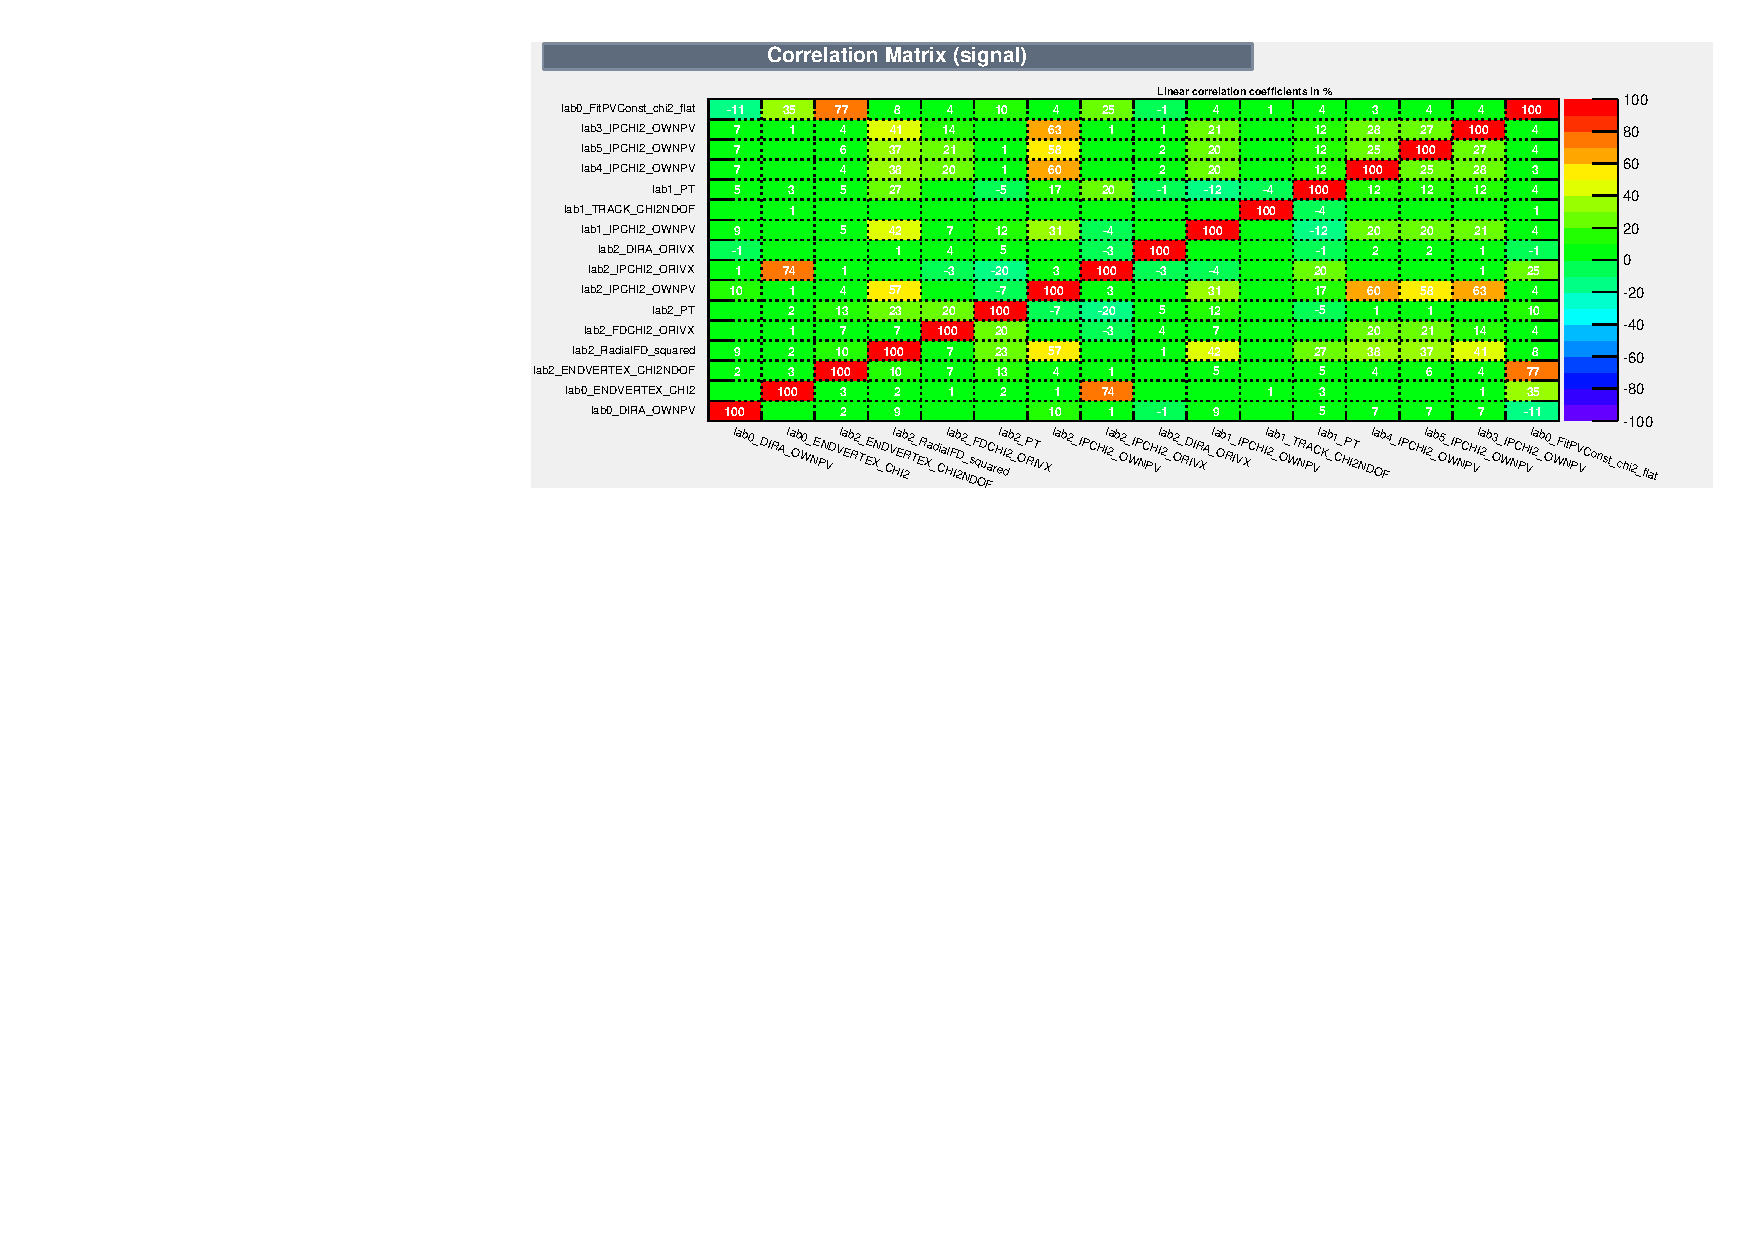
\includegraphics[width=0.85\textwidth]{02Selection/figs/CorrelationMatrixS.pdf}\\
		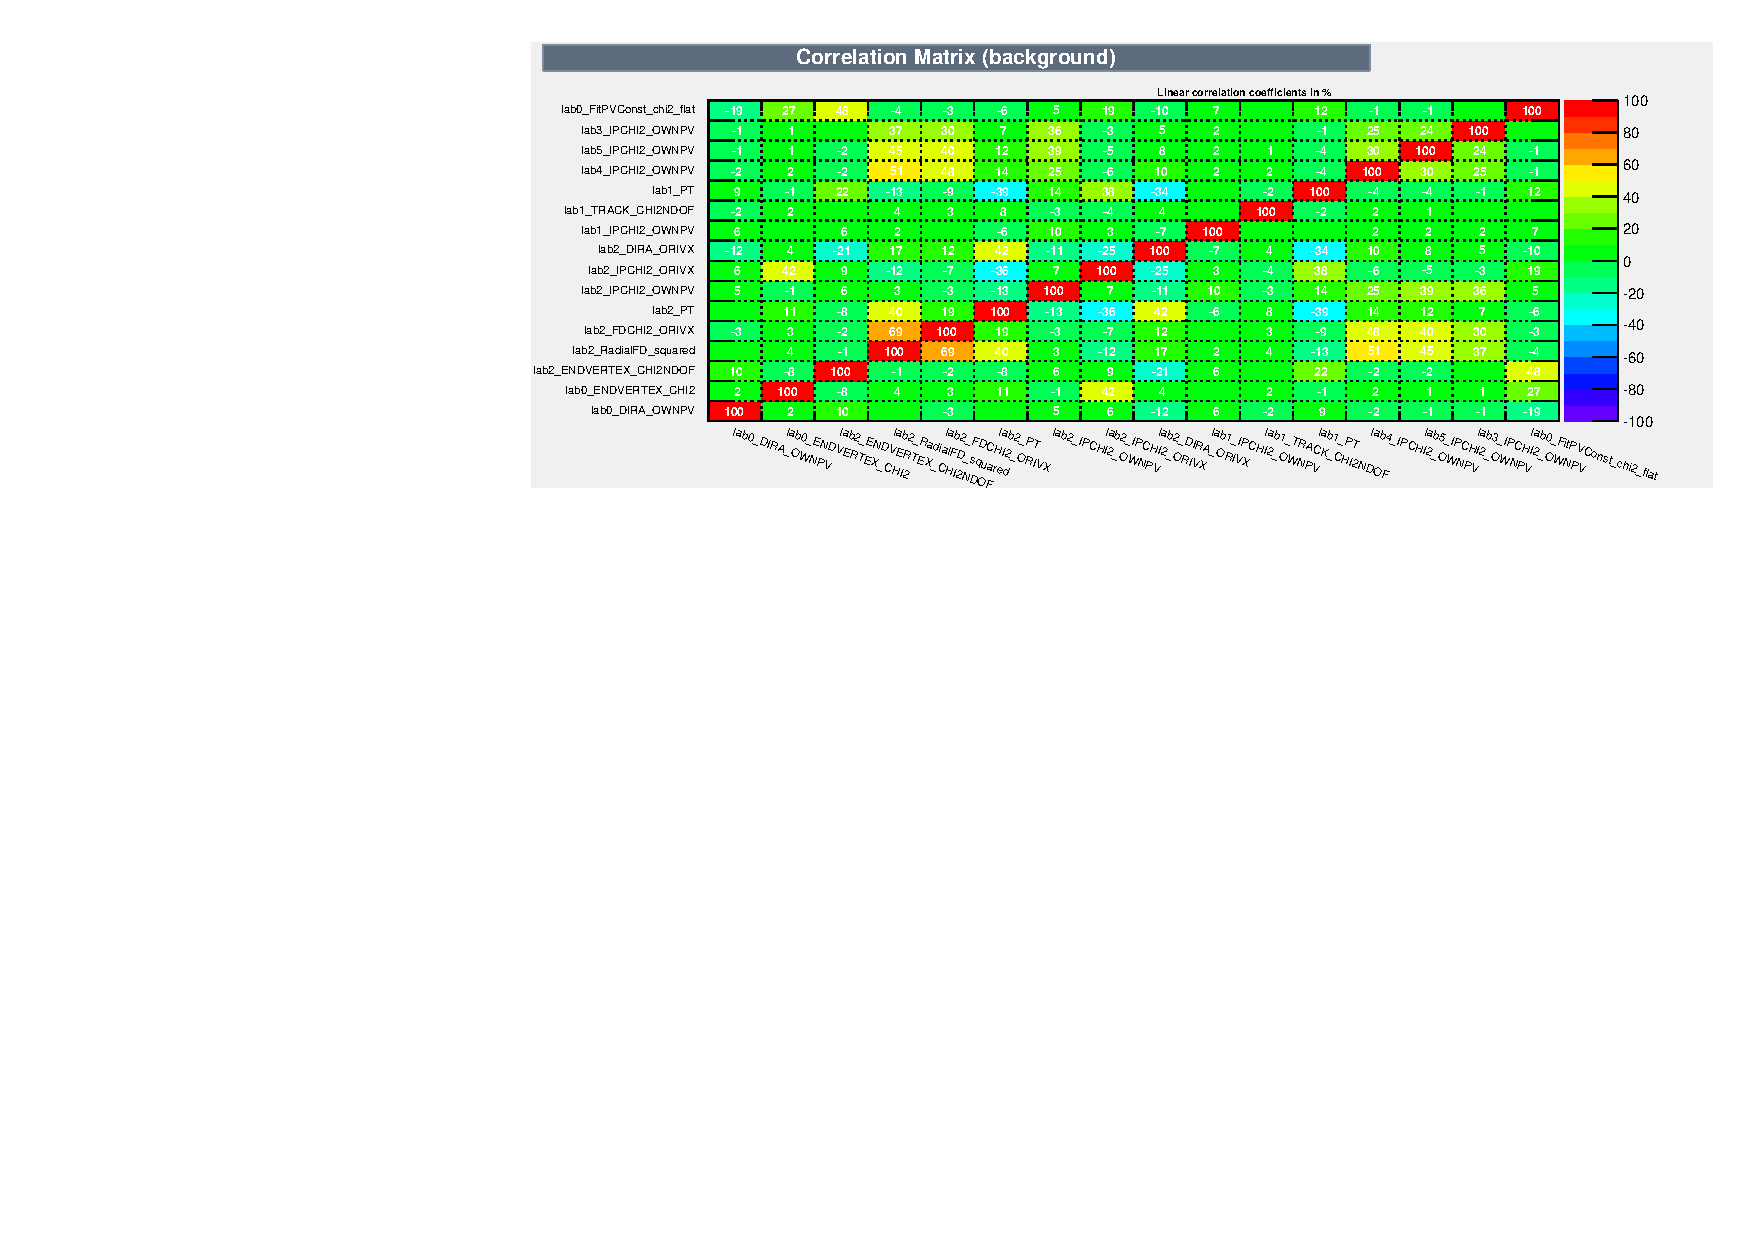
\includegraphics[width=0.85\textwidth]{02Selection/figs/CorrelationMatrixB.pdf}
	\end{center}
        \vspace{-2mm}
	\caption{Correlation matrices of the input features used in the training of the
	BDT for signal (top) and background (bottom).}
	\label{fig:BDTcorrelation}
\end{figure}
%

The BDT implementation of TMVA \cite{hocker:2007ht} is used. The BDT is built
out of 1700 trees, with a depth limited to four. For each node, at least
$\SI{2.5}{\percent}$ of the training events have to be present. The chosen boosting method is the
AdaBoost \cite{AdaBoost} algorithm with a boost factor $\beta=\num{0.5}$. 
The number of trees and the maximal depth of trees have been increased
iteratively until no significant increase of the performance without overtraining was observed.
The BDT is tested on the events that are not used in the training. The plot of
this overtraining check is given in Fig.~\ref{fig:BDTovertraining}.
\begin{figure}[t]
	\begin{center}
		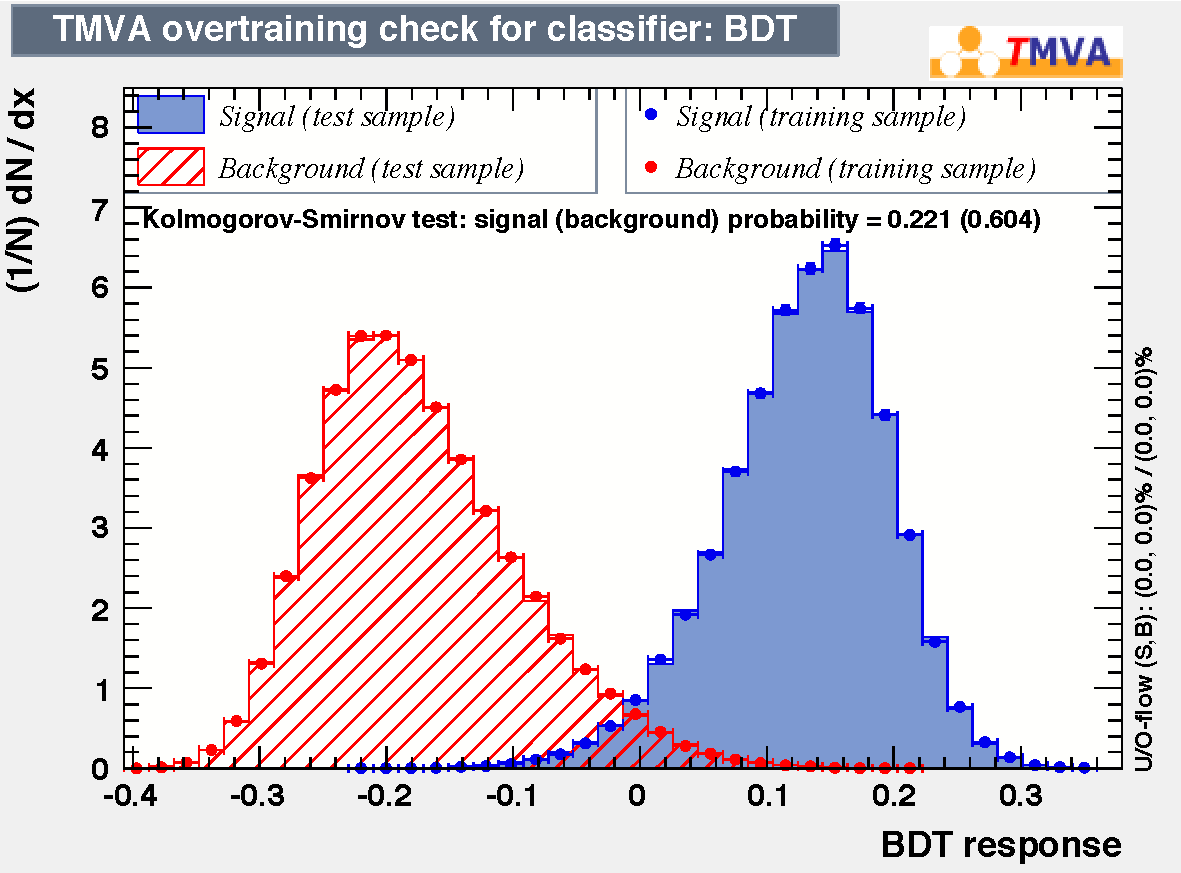
\includegraphics[width=0.6\textwidth]{02Selection/figs/overtrain_BDT.pdf}
	\end{center}
        \vspace{-2mm}
	\caption{Distributions of the BDT response on training and test samples.}
	\label{fig:BDTovertraining}
\end{figure}

%===============================================================================
\subsection{BDT selection optimisation}
\label{sec:BDToptimisation}

To estimate the best requirement on the output of the BDT classifier, the
statistical uncertainty of the \CP~coefficients derived from the analysis of
simulated samples is used as the figure of merit (FoM). To determine the
sensitivity, the preselection, the mass vetoes and the wrongly associated PV veto
are applied and the BDT classifier is calculated for every candidate. The BDT
cut point is then scanned with a step size of $\num{0.01}$ from
\numrange{-0.15}{0.10} and a step size of \num{0.05} in the outer regions. For
each cut point, a simulated (\emph{toy}) sample is generated. This
sample contains the same signal and combinatorial background yields as determined
from the real dataset via a maximum likelihood fit of the $\Bz$ mass distribution.
Finally, a time-dependent analysis of each toy dataset is performed in order to
estimate the statistical uncertainty on $S_f$ and $S_{\bar f}$.
These statistical uncertainties as a function of the BDT cut are shown in Fig.~\ref{fig:BDToptimum}. Based on
these distributions, the BDT cut point is chosen to be at \num{0.05}.
\begin{figure}[htbp]
	\begin{center}
		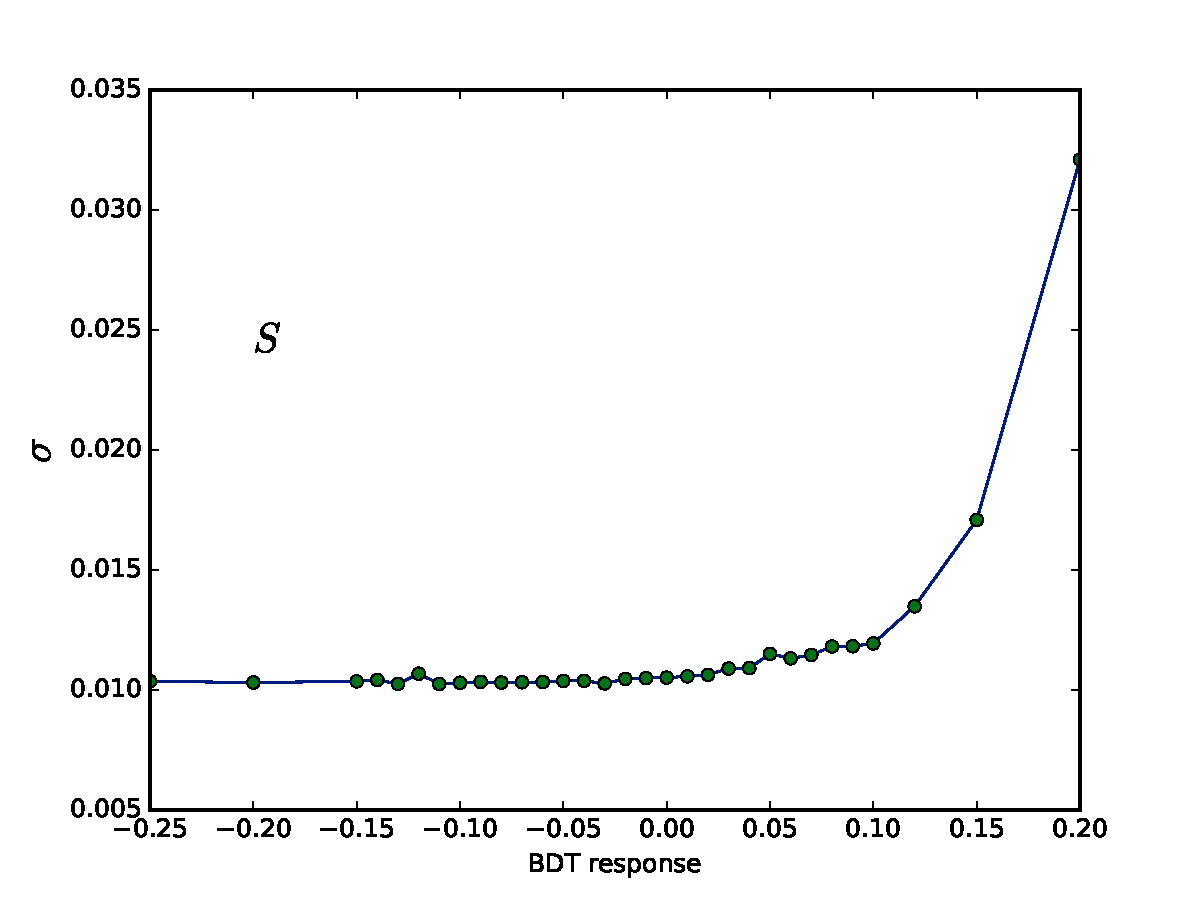
\includegraphics[width=0.49\textwidth]{02Selection/figs/sensitiv_Sf.pdf}
		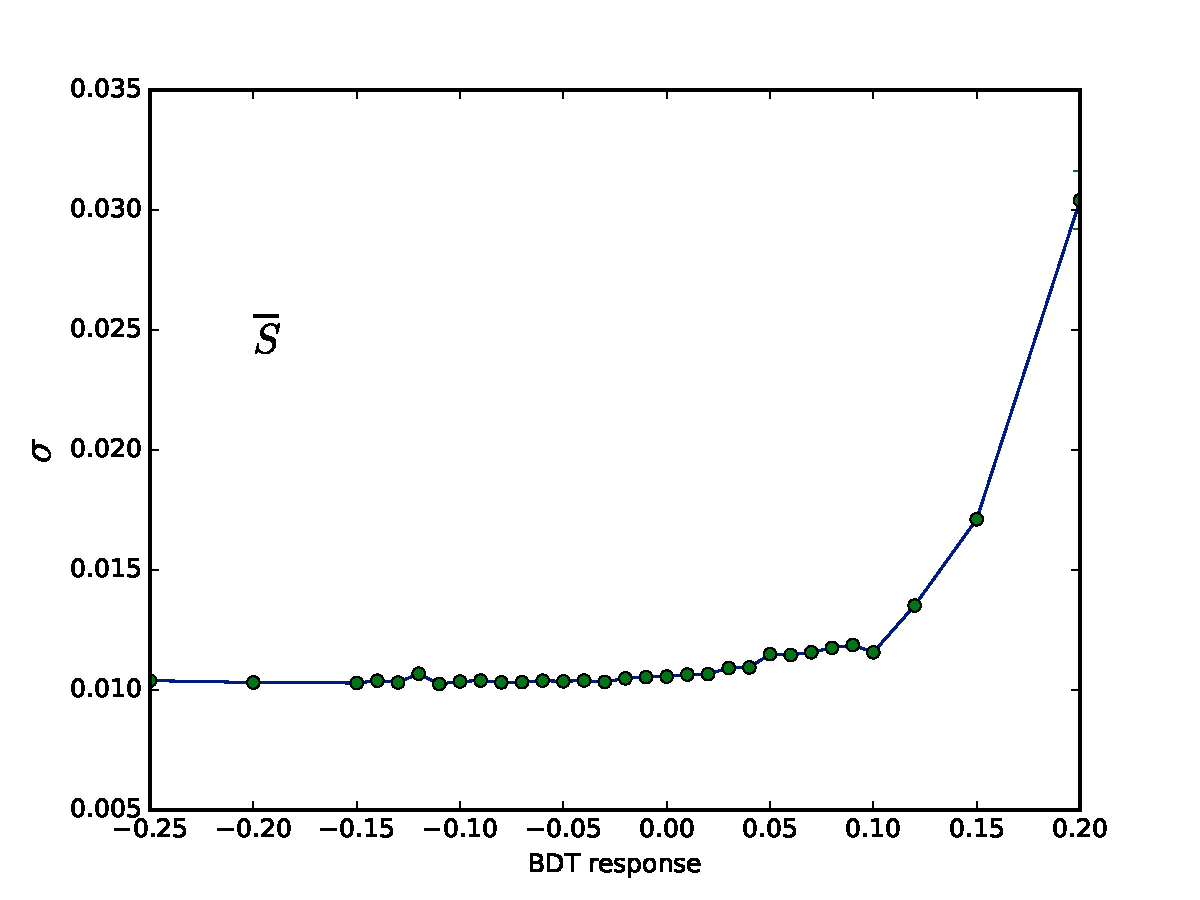
\includegraphics[width=0.49\textwidth]{02Selection/figs/sensitiv_Sfbar.pdf}
	\end{center}
        \vspace{-4mm}
	\caption{Expected statistical uncertainty on of $S_f$ (left) and $S_{\bar f}$ (right) as a function of
	the cut on the output of the BDT classifier, as obtained from simulated samples.}
	\label{fig:BDToptimum}
\end{figure}

%===============================================================================
\subsection{Multiple candidates}
\label{sec:multiplecandidates}

After the stripping selection and trigger requirements, approximately $9\%$ of the events contain at least two
$\Bz$ candidates, and $18-20\%$ of all $\Bz$ candidates share
an event. If the offline selection is also applied, around $0.4\%$ of
the events contain multiple $\Bz$ candidates, and $0.8\%$ of all
$\Bz$ candidates share an event. More details are given in
Appendix~\ref{app:multiplecandidates}. In order to be consistent
with the prescription used in the stripping and trigger requirements, only the
best PV is chosen; all events in which the best PV is no longer present after
the offline selection are removed. Finally, since the remaining $\Bz$ candidates are considered to be equally likely
signal candidates, a single $\Bz$ candidate per event is chosen randomly following
the prescription of Ref.~\cite{multipleCandidates}, which prevents any unexpected bias due to a more specific choice.

%===============================================================================
\subsection{Selection performance}
\label{sec:overallofflineselectionperformance}

The offline selection performances are listed in Table~\ref{tab:offlineselperformance}.
They are determined by using data candidates of the $\num{2012}$ sample with an
invariant $\Bz$ mass above $\SI{5500}{\MeVcc}$ to represent combinatorial
background, and signal MC candidates (see Sec.~\ref{sec:MC}) to represent the signal.
%
\iffalse
\begin{figure}[t]
	\begin{center}
		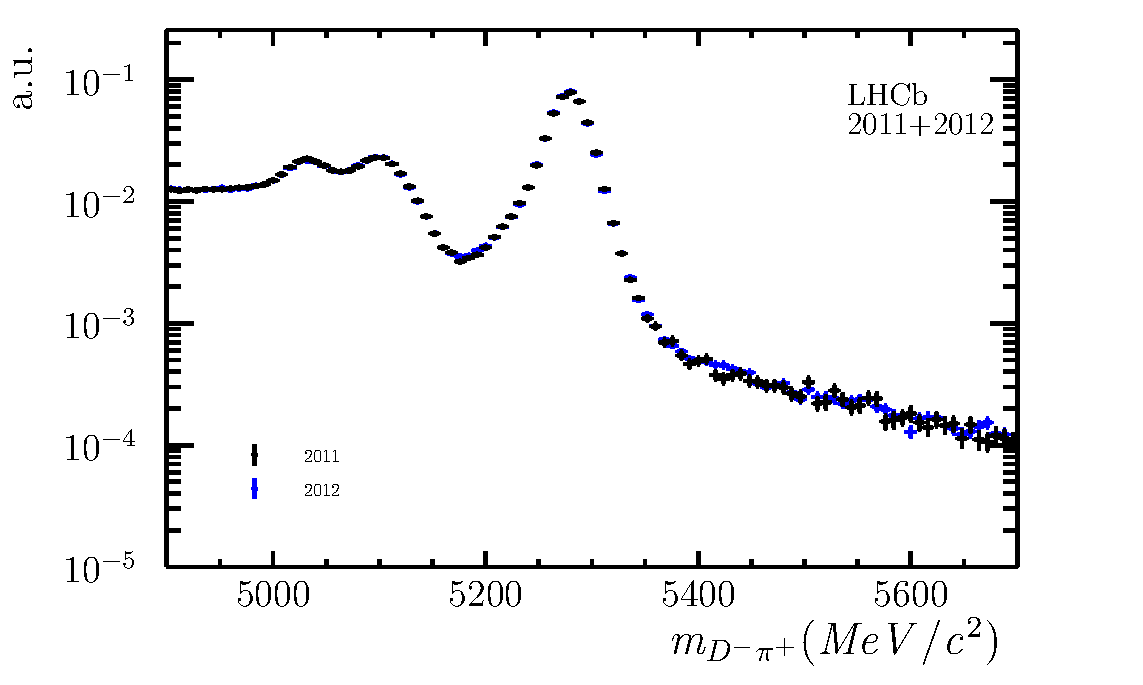
\includegraphics[width=0.55\textwidth]{02Selection/figs/BmassAfterSelection.pdf}
	\end{center}
        \vspace{-2mm}
	\caption{Mass distributions of the $\Bz\to\Dmp\pipm$ candidates passing the full offline selection for the \num{2011} (blue) and \num{2012} (black) data samples.}
	\label{fig:BMassAfterSelection}
\end{figure}
\fi
%
\begin{table}[t]
	\centering
	\caption{Signal efficiencies and
	background rejections of the different selection steps given with
	respect to the previous selection step. The preselection efficiency is computed  w.r.t. the number of candidates passing trigger and stripping requirements.
	The last row shows the overall
	selection performance without the multiple candidate removal.}
	\begin{tabular}{ccc}
		\toprule
		Selection step & $\varepsilon_\text{sig}$ & $1-\varepsilon_\text{bkg}$ \\
		\midrule
		preselection & \SI{93.61\pm0.06}{\percent} & \SI{85.20\pm0.02}{\percent} \\
		$\Lambda_c^\mp$ veto & \SI{93.48\pm0.06}{\percent} & \SI{9.85\pm0.03}{\percent} \\
		semileptonic veto & \SI{98.96\pm0.03}{\percent} & \SI{7.66\pm0.03}{\percent}\\
		wrongly associated PV veto & \SI{97.75\pm0.04}{\percent} & \SI{15.81\pm0.04}{\percent}\\
		BDT selection & \SI{83.63\pm0.10}{\percent} & \SI{97.18\pm0.01}{\percent}\\
		\midrule
		total & \SI{70.7\pm0.1}{\percent} & \SI{99.911\pm0.002}{\percent}\\
		\bottomrule
	\end{tabular}
	\label{tab:offlineselperformance}
\end{table}
%
Additionally, the BDT performances are quoted in Table~\ref{tab:BDTperfomancesplit} split by magnet polarity and year of data taking.
\begin{table}[t]
	\small
	\centering
	\caption{BDT performance for each magnet polarity (up and down) and year of data taking. The
	quoted efficiencies contain signal and background.}
	\begin{tabular}{@{}c@{\hspace{-2mm}}cccc@{}}
		\toprule
		& \num{2011}, up & \num{2011}, down & \num{2012}, up & \num{2012}, down \\
		\midrule
		\# cand.\ before BDT & \num{398357} & \num{569853} & \num{1301800} & \num{1316597} \\
		\# cand.\ after BDT & \num{210844} & \num{285137} & \num{601345} & \num{609880} \\
		$\varepsilon_{\text{sig}+\text{bkg}}$ & \SI{50.67\pm0.08}{\percent} & \SI{50.04\pm0.07}{\percent} & \SI{46.19\pm0.04}{\percent} & \SI{46.32\pm0.04}{\percent} \\
		\bottomrule
	\end{tabular}
	\label{tab:BDTperfomancesplit}
\end{table}
Finally, in order to check the contribution of non-resonant
$\Bz\to\Kp\pim\pim\pip$ decays, the $\Bz$ and $\Dmp$ invariant mass
distributions are analysed after applying the full offline selection 
(with the exception of the $\Bz$ and $\Dmp$ mass cuts)
in two ways. First, the $\Dmp$ mass distribution is plotted 
for candidates falling in a $\Bz$ mass signal window
(Fig.~\ref{fig:NonResonant_BmassCut}). From this plot, the maximal contamination from non-resonant decays can be
estimated to be roughly $\SI{1}{\percent}$.
\begin{figure}[t]
	\begin{center}
		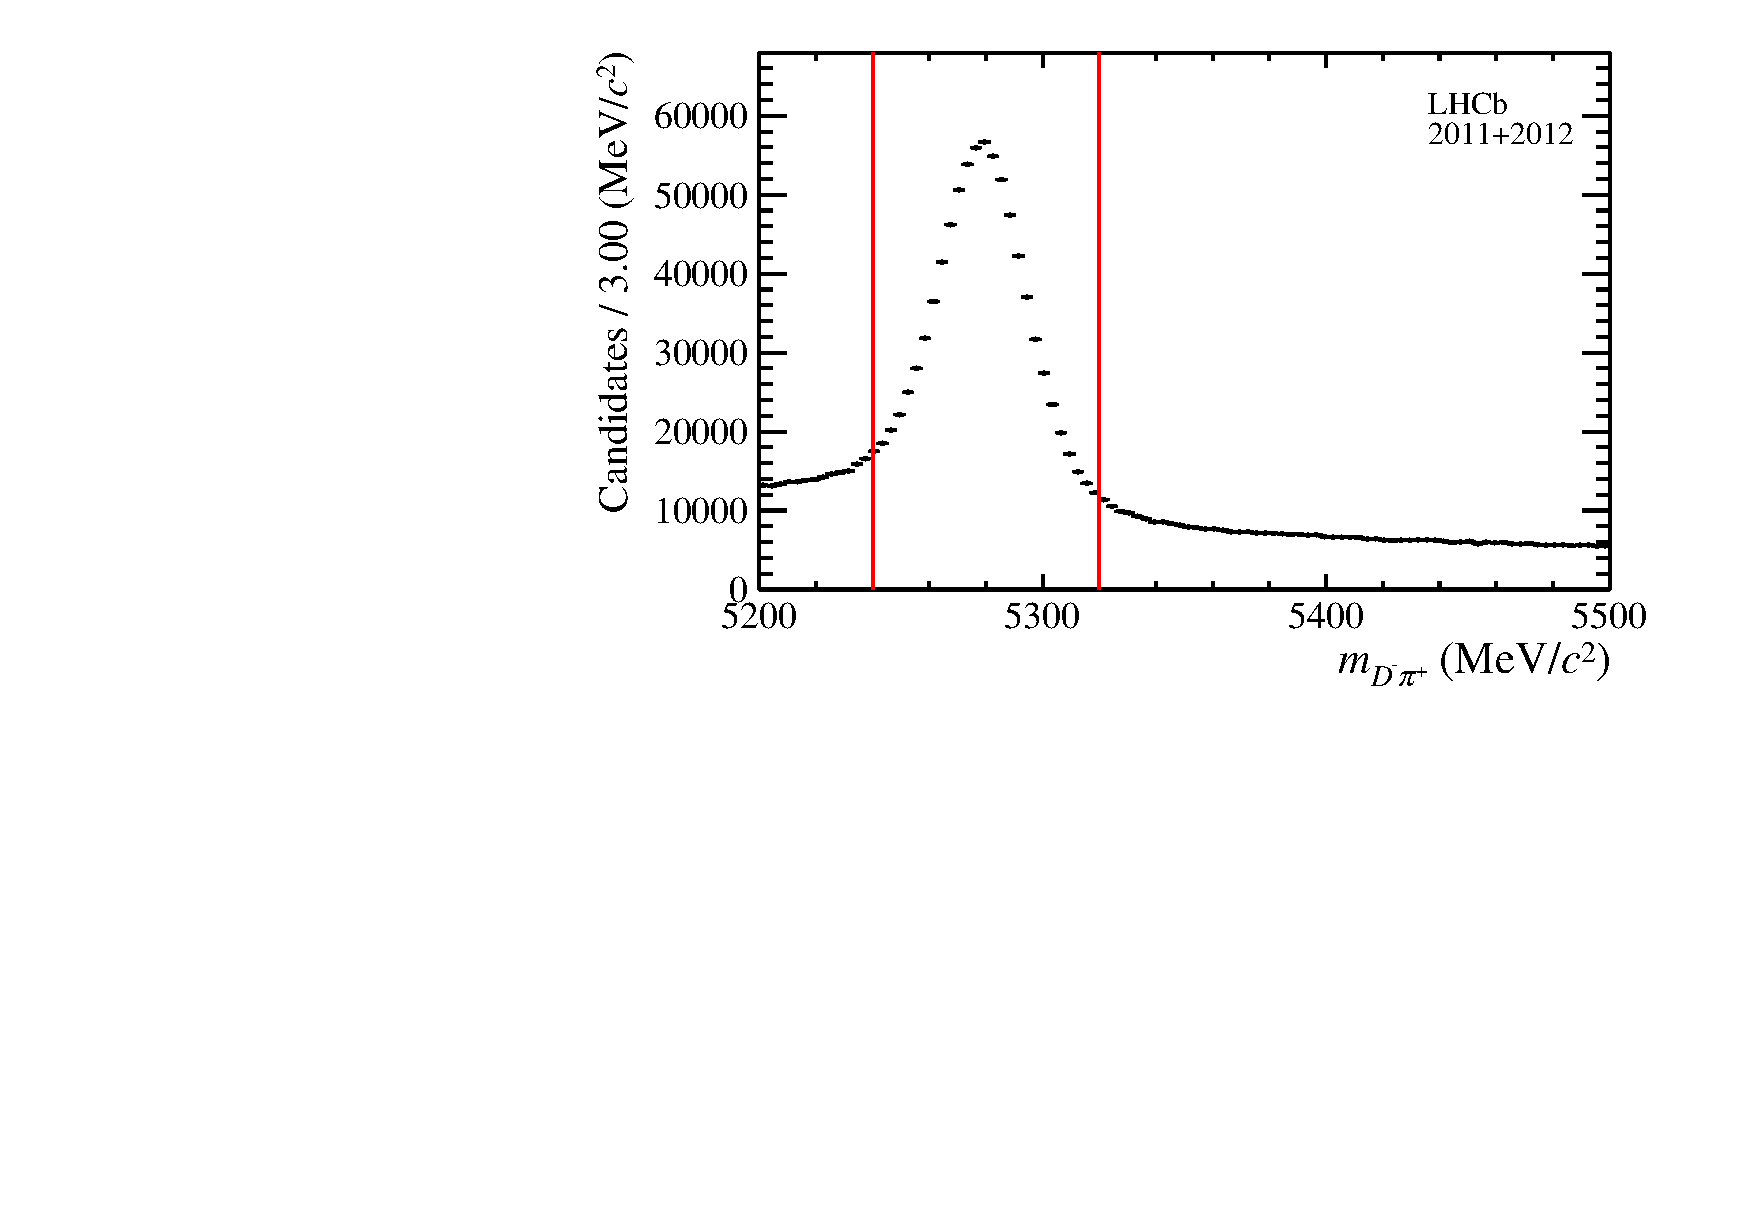
\includegraphics[width=0.49\textwidth]{02Selection/figs/BmassCut.pdf}
		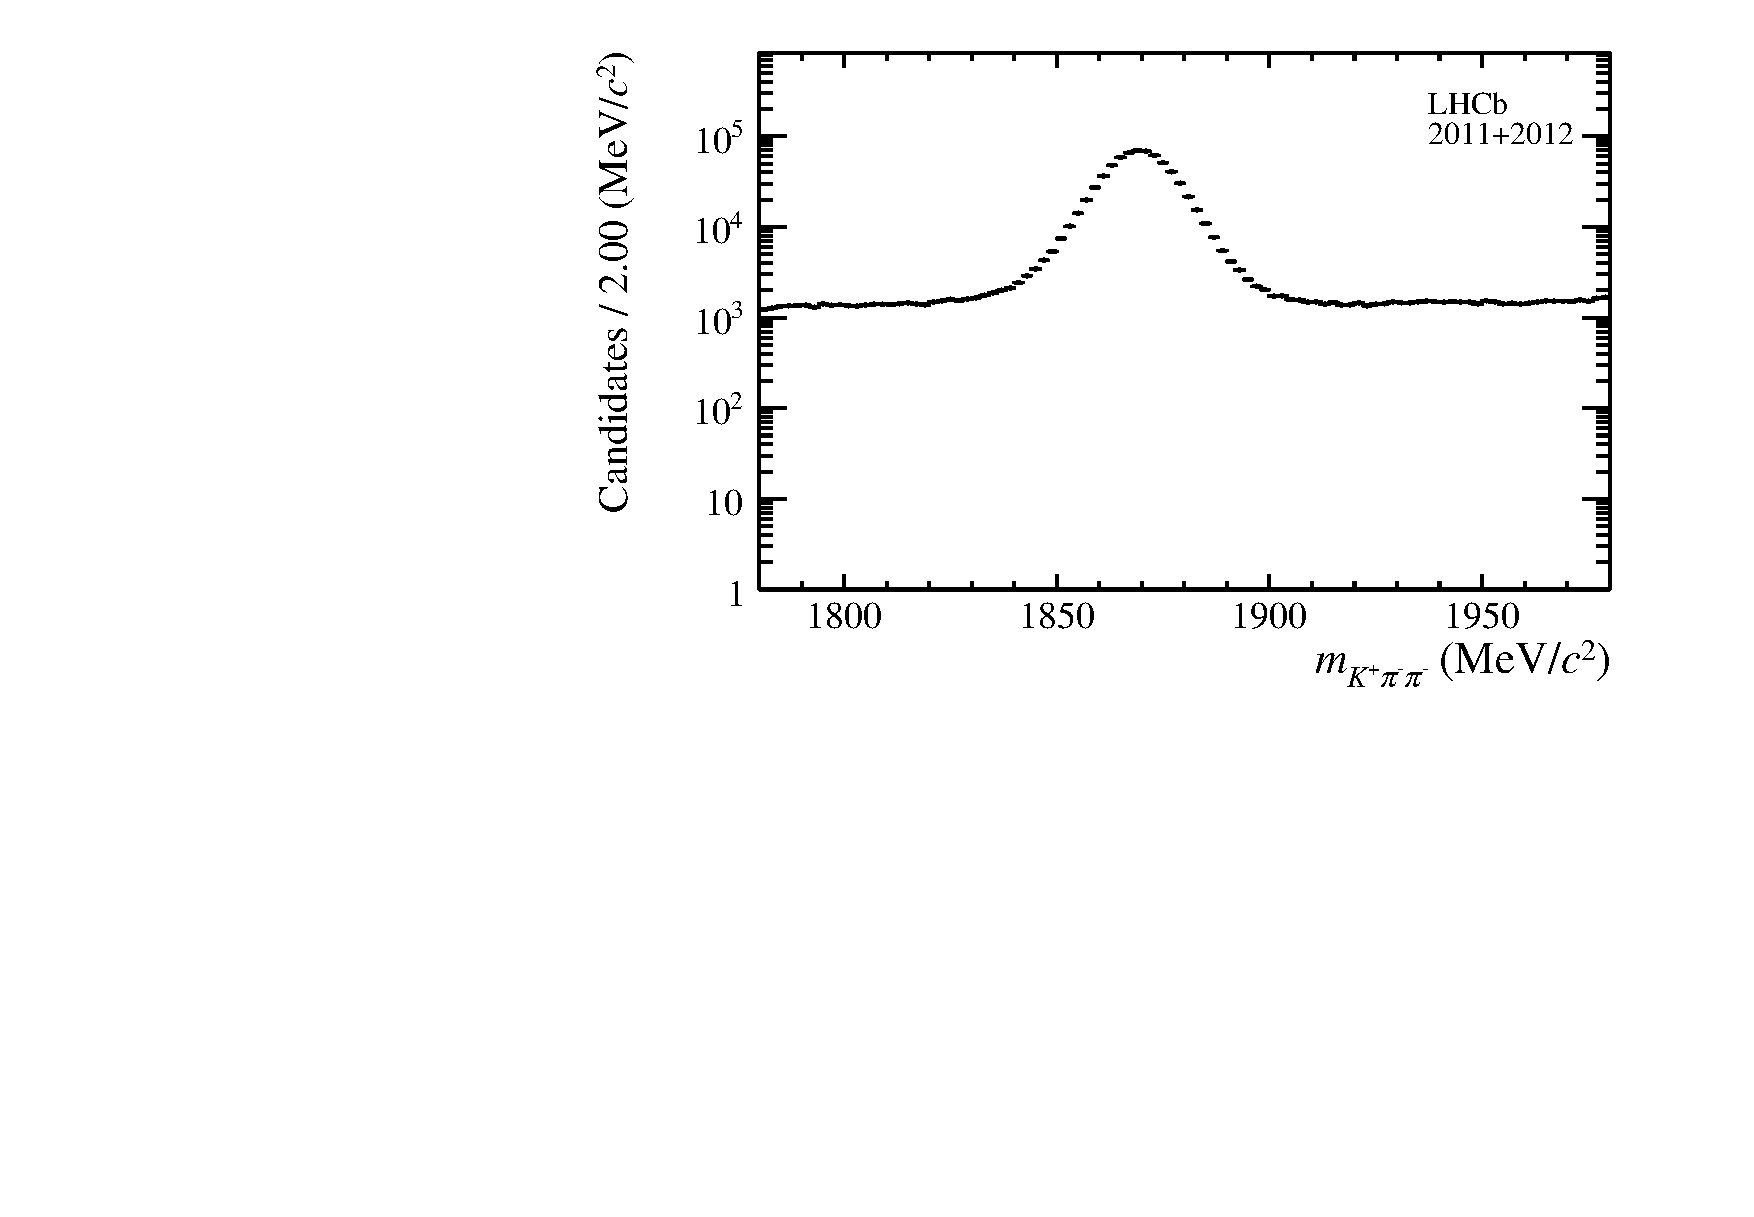
\includegraphics[width=0.49\textwidth]{02Selection/figs/Resulting_Dmass.pdf}
	\end{center}
        \vspace{-2mm}
	\caption{Left: $\Bz$ mass distribution with red vertical lines indicating the
	selected signal window. Right: resulting
	\Dmp~mass distribution in the \Bz~signal window.}
	\label{fig:NonResonant_BmassCut}
\end{figure}
%
Then, the $\Bz$ distribution after excluding the $\Dmp$ signal
window is plotted. To quantify the non-resonant $\Bz\to\Kp\pim\pim\pip$ decays, the
sum of an exponential and a Gaussian with a fixed shape is used to fit the resulting $\Bz$ mass
distribution, as shown in Fig.~\ref{fig:NonResonant_DmassCut}. As the fitted
$\Bz$ yield is $\num{645\pm242}$, the non-resonant contribution is
assumed to be negligible.
\begin{figure}[t]
	\begin{center}
		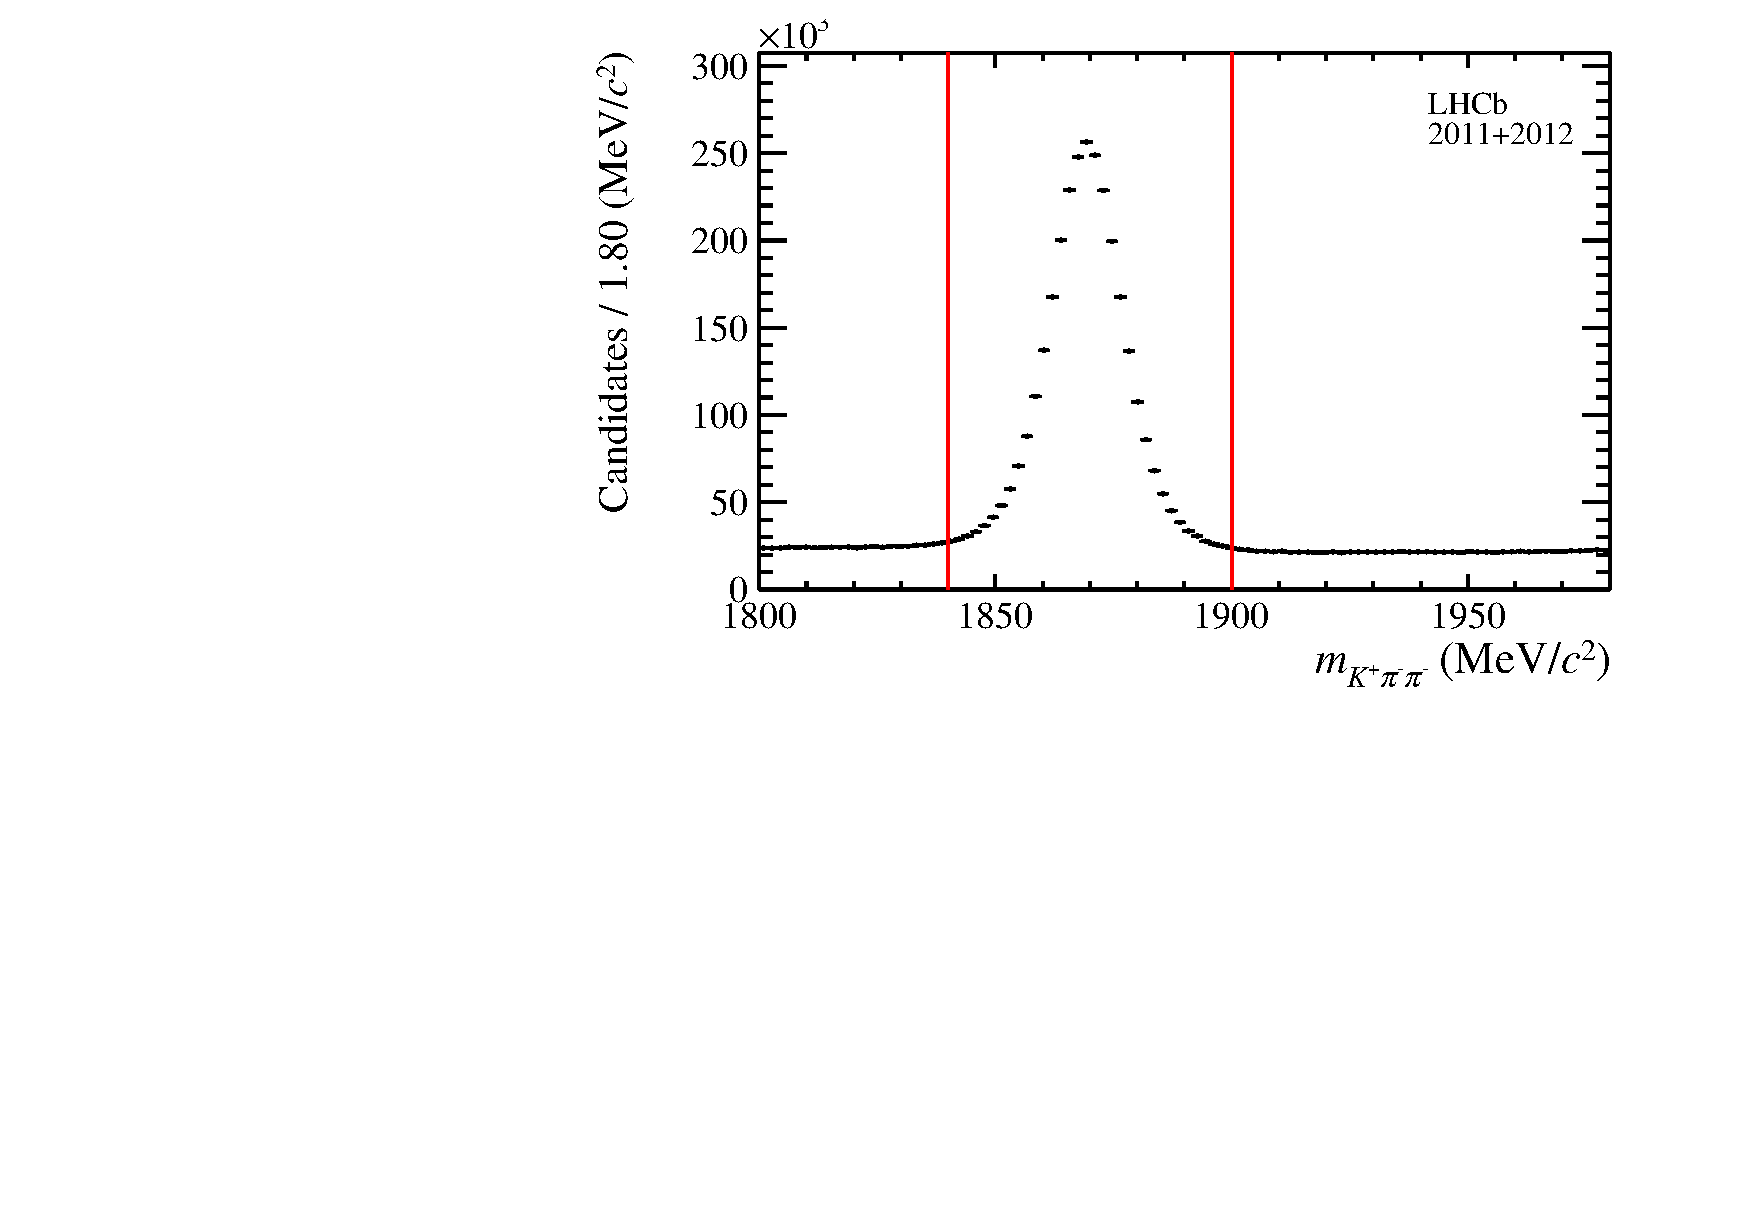
\includegraphics[width=0.49\textwidth]{02Selection/figs/DmassCut.pdf}
		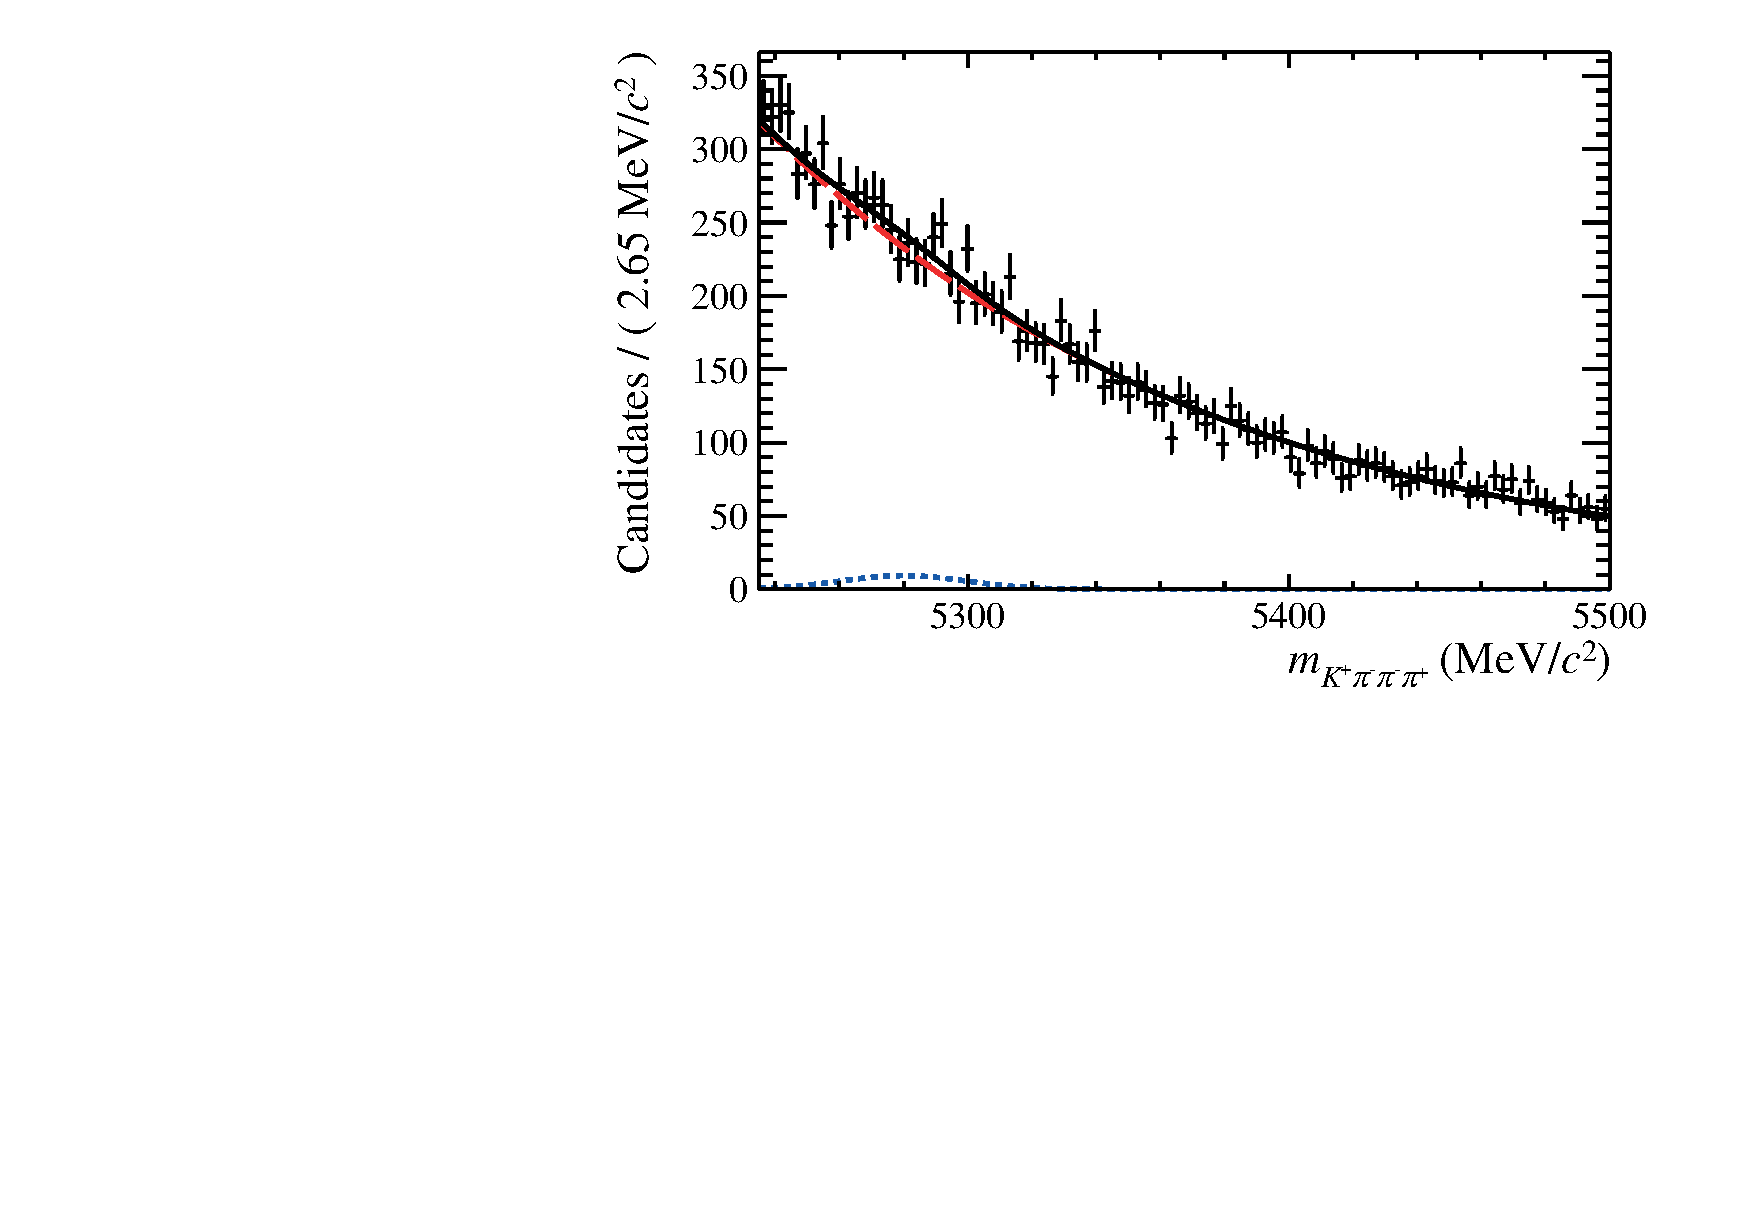
\includegraphics[width=0.49\textwidth]{02Selection/figs/Resulting_Bmass.pdf}
	\end{center}
        \vspace{-2mm}
	\caption{Left: $\Dmp$ mass distribution with red vertical lines indicating the
	excluded range. Right:
	\Bz~mass distribution outside the \Dmp~mass window with the fitting function overlaid.}
	\label{fig:NonResonant_DmassCut}
\end{figure}

%===============================================================================
\section{Simulation and expected sample composition}
\label{sec:MC}

Simulated samples are used to (i) gain a detailed overview of all sources of
$b$-hadron decays that contribute to the sample and (ii) model the relevant
distributions studied in the analysis. Simulated data undergoes the same
reconstruction and selection as real data. Each sample
is split into four subsamples according to magnet polarity (up or down) and year of data taking (2011 or 2012),
in proportions similar to those present in real data.

The simulated samples used are listed in Table~\ref{tab:MC_samples}, together with the
number of true signal events passing the final selection and the corresponding
total efficiencies. The PID requirements on the bachelor pion are not is applied in order to
compute these efficiencies.
\begin{table}[t]
	\centering
	%\resizebox{\textwidth}{!}{
	\begin{tabular}{lcrc}
		\toprule
		Sample 				& Event type & \multicolumn{1}{c}{$N_\text{sel}$} & Efficiency [\%] \\
		\midrule
		$\Bz\to \Dmp\pipm$ 		& $11164003$ & $101096$ & $1.966\pm0.006$ 	\\
		$\Bz\to \Dm\Kp$ 		& $11264011$ & $19300$ 	& $1.833\pm0.013$ 	\\
		$\Bz\to \Dmp\rho^\pm$ 	& $11164401$ & $2408$ 	& $0.1178\pm0.0024$ 	\\
		$\Bz\to D^{*\mp}\pipm$ 	& $11164404$ & $14901$ 	& $0.721\pm0.006$ 	\\
		$\Bs\to \Dsm\pip$ 	& $13264021$ & $7942$ 	& $0.1531\pm0.0017$ \\
		$\Lb\to \L_c^{+}\pim$ 	& $15164001$ & $325$ 	& $0.0155\pm0.0009$ \\
		$\Bz\to \Dm K^{*+}$ 	& $11164470$ & $361$ 	& $0.0358\pm0.0019$ 	\\
		\bottomrule
	\end{tabular}
	%}
	\caption{Samples of simulated data used in the analysis, with the numbers of candidates
	$N_\text{sel}$ after the final selection, and the selection efficiencies. Efficiencies
	include generator level, trigger, stripping, offline selection and tagging efficiencies.
        The $\Bz\to \Dmp\pipm$ signal sample is generated with the parameters given in Appendix~\ref{app:mcgen}.}
	\label{tab:MC_samples}
\end{table}

%-------------------------------------------------------------------------------
\subsection{PID$K$ correction}
\label{sec:pid}

The $\PIDK$ distributions in data and MC differ. To correct for that,
the $\PIDK$ distributions in MC are resampled using the binned $\PIDK$
probability density functions of dedicated calibration samples. 
These calibration samples consist of kinematically clean $D^{*+}\to
\Dz(\to \Km\pip)\pip$ decays, for which no requirement on RICH
information is applied in the reconstruction.

The need for this resampling is due to the fact that, if the same cut is applied
on data and MC, the resulting distributions in other observables may
differ if the $\PIDK$ distributions in data and MC are different.
Moreover, a correct $\PIDK$ distribution in MC allows the proper
estimation (on MC) of the efficiency or misidentification rate for a given
$\PIDK$ cut, which is an essential ingredient in the fit to the $\Bz$ invariant
mass distribution (as described in Sec.~\ref{sec:massfit}).

The following strategy is adopted. A two-dimensional binning in momentum, $p$,
and pseudorapidity, $\eta$, is defined. For each bin, the corresponding $\PIDK$
distribution in the calibration sample is built and for each event in the MC sample, 
a random $\PIDK$ value is sampled from the $\PIDK$ distribution
associated with the corresponding bin in the calibration sample. More details are
given in Appendix~\ref{app:pid}.

Because of the $\Lambda_{c}^\mp$ veto described in Sec.~\ref{sec:vetoes}, the PID$p$
variable for the $\Dmp$ daughter particles is resampled as well in a similar manner
using $\Lambda^{0}\to p\pim$ decays as calibration channel.

The nominal binning used for the PID resampling is the following:
\begin{itemize}[noitemsep,topsep=0pt]
  \item momentum: $100$ uniform bins between $2~\gevc$ and $200~\gevc$, two equal bins between $200~\gevc$ and $300~\gevc$;
  \item pseudorapidity:~one~bin~between~$1.5$~and~$1.55$,~$69$~uniform~bins~between~$1.55$~and~$5.0$.
\end{itemize}
In order to check the robustness of the method and evaluate a systematic uncertainties, two alternative binning schemes are defined:
\begin{itemize}[noitemsep,topsep=0pt]
  \item \emph{narrow} binning: the number of bins in the uniform binning parts for $p$ and $\eta$ are increased to $140$ and $80$, respectively;
  \item \emph{wide} binning: the number of bins in the uniform binning parts for $p$ and $\eta$ are decreased to $60$ for both.
\end{itemize}
The $\PIDK$ variable is resampled for the $\Bz\to\Dmp\pipm$ and $\Bz\to\Dmp K^{\pm}$ Monte Carlo samples using these two alternative schemes as well. 
The result of this resampling is shown in Fig.~\ref{fig:pidkresampling} for $\Bz\to\Dmp\pipm$ decays.
The effect on all the other physics background is expected to be very small and thus neglected, since they are all located in different regions of the $\Dmp\pipm$ invariant mass. More details on this will be given in Secs.~\ref{sec:massfit} and~\ref{sec:systematics}.
\begin{figure}[t]
        \begin{center}
                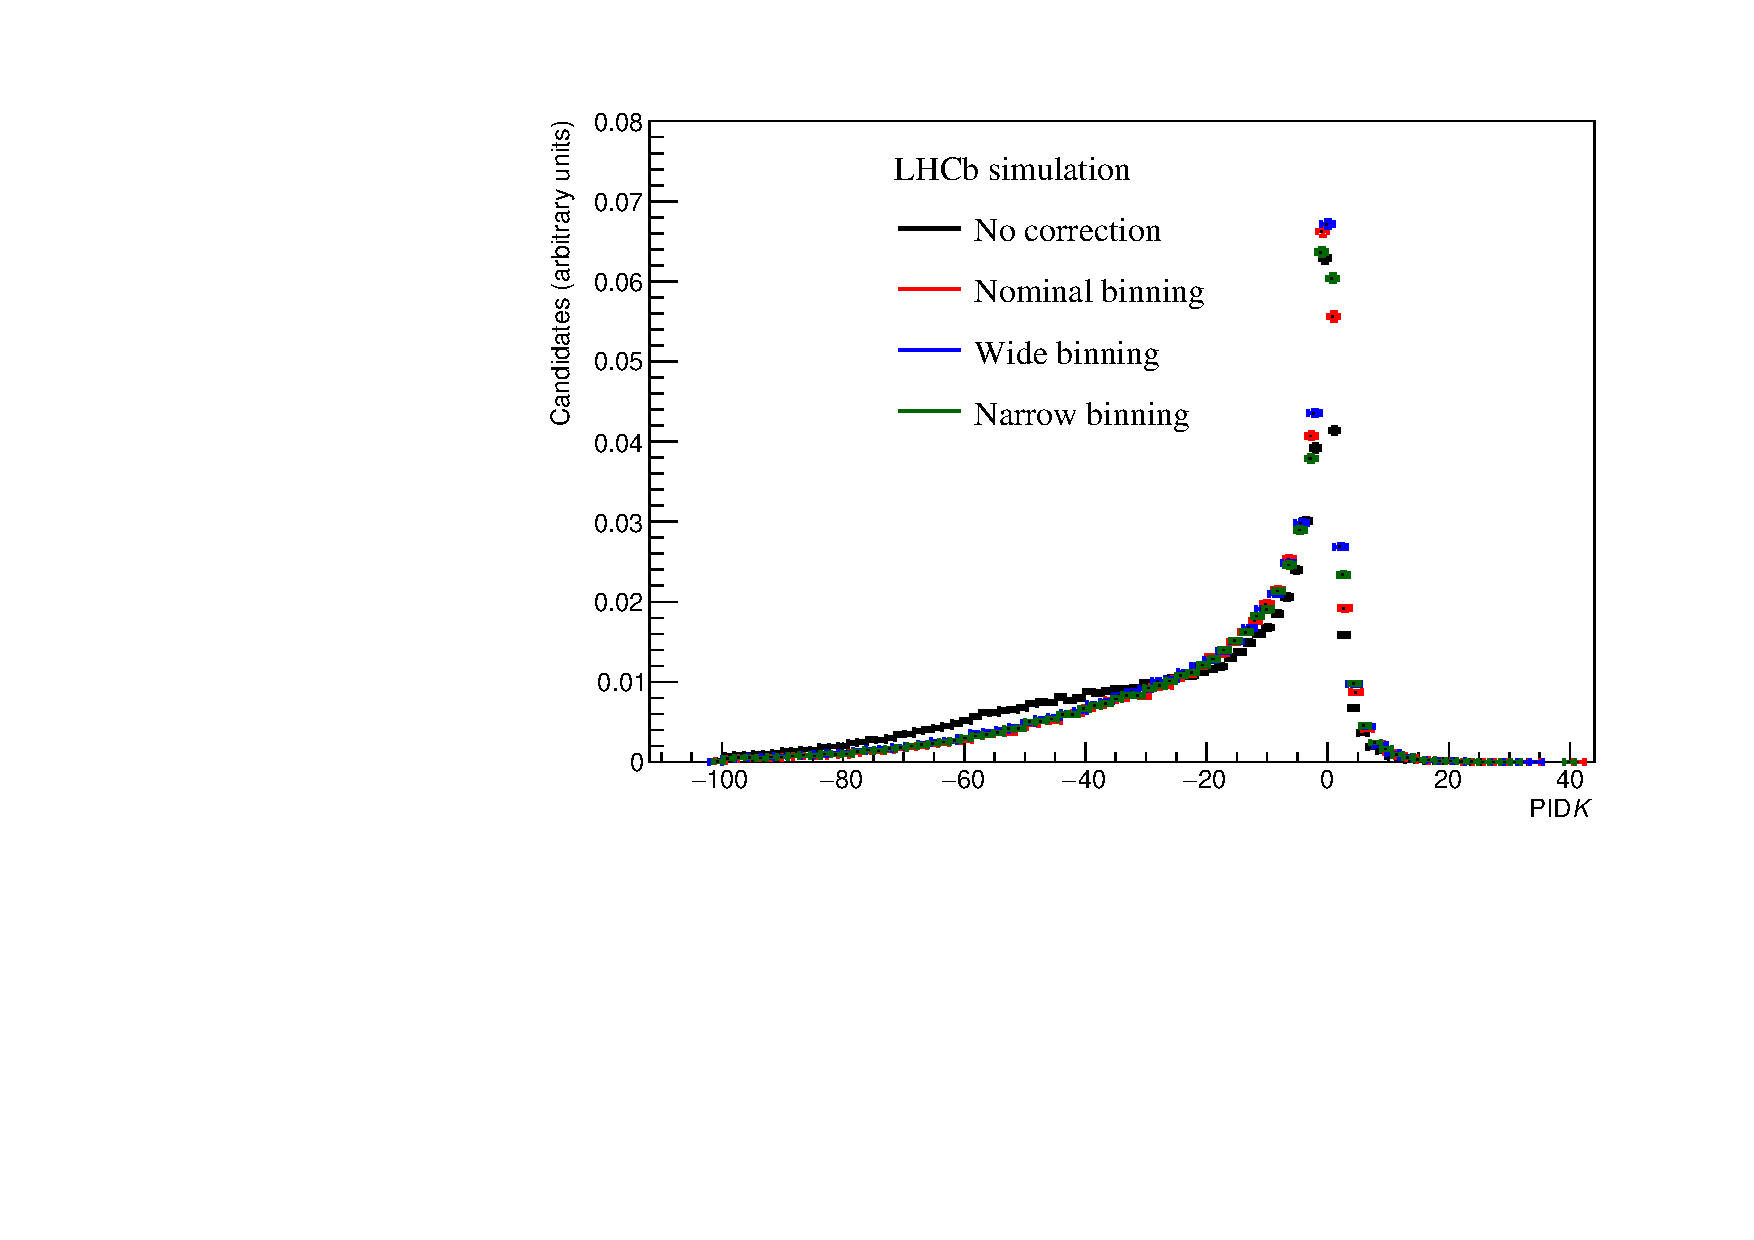
\includegraphics[width=0.7\textwidth]{02Selection/figs/PIDK_check_binning.pdf}
        \end{center}
        \vspace{-2mm}
        \caption{$\PIDK$ distribution for simulated $\Bz\to\Dmp\pipm$ decays without resampling (black), after the nominal resampling (red),
        after the resampling with the wide binning scheme (blue), and after the resampling with the narrow binning scheme (green).}
        \label{fig:pidkresampling}
\end{figure}

%-------------------------------------------------------------------------------
\subsection{Surviving physics backgrounds}

Some physics background candidates that survive the selection chain described in
the previous section are expected. In the pion sample, these are:
%
\begin{itemize}[noitemsep,topsep=0pt]
	\item \boldmath{$\Bz\to D^{-}K^{+}$}: Peaking background due to the bachelor kaon being wrongly identified as a pion.
	\item \boldmath{$\Bz\to D^{\mp}\rho^{\pm}(\to\pi^{\pm}\pi^{0})$}: Low mass background due to a missing neutral pion in the reconstruction.
	\item \boldmath{$\Bz\to D^{*\mp}(\to D^{\mp}\gamma/\pi^{0})\pi^{\pm}$}: Low mass background due to a missing neutral particle in the reconstruction.
\end{itemize}
%
In the kaon sample, the following backgrounds are expected:
%
\begin{itemize}[noitemsep,topsep=0pt]
	\item \boldmath{$\Bz\to D^{\mp}\pi^{\pm}$}:
		Signal candidates having the bachelor pion wrongly identified as a kaon.
	\item \boldmath{$\Bz\to D^{\mp}\rho^{\pm}(\to\pi^{\pm}\pi^{0})$}:
		Low mass background where, in addition to the missing pion in the final state, a reconstructed pion is
		wrongly identified as a kaon.
	\item \boldmath{$\Bz\to D^{-}K^{*+}(\to\pi^{0}K^{+})$}:
		Low mass background where the neutral pion is missing in the reconstruction.
\end{itemize}
%
The background fractions expected in the pion sample with respect to the
$\Bz\to\Dmp\pipm$ signal are reported in Table~\ref{tab:expected-backgrounds}. These
fractions are computed using the branching fractions of the expected decay as
inputs and from the ratio of efficiencies estimated from MC and corrected as described in Sec.~\ref{sec:pid}. Where
relevant we consider also the ratio of the fragmentation probabilities of $b$
quarks to different $b$ hadrons, which are $34.0\pm2.1\%$, $21.8\pm4.7\%$ and $10.1\pm1.5\%$ 
for $\Bz$, $\Bs$ and $\Lambda^0_b$, respectively~\cite{HFLAV16}. 
These expectations will be compared with the
results from the fit to data described in the next section.
\begin{table}[t]
	\centering
	%\resizebox{\textwidth}{!}{
	\begin{tabular}{lrrr}
		\toprule
		Decay & $\mathcal{B}$ from Ref.~\cite{PDG2017} [\%] & $\epsilon_{\rm bkg}$ [\%] & $f_{\rm bkg}$ [\%] \\
		\midrule
		$\Bz\to\Dm\Kp$ 			  			      & $0.00186\pm0.00020$ & $0.684\pm0.008$   & $2.61\pm0.31$ \\
		$\Bz\to\Dmp\rho^\pm(\to\pipm\pi^0)$ 			      & $0.071\pm0.011$     & $0.1149\pm0.0024$ & $16.7\pm2.8$  \\
		$\Bz\to D^{\mp*}(\to\Dmp\gamma/\pi^{0})\pipm$ 	  & $0.0080\pm0.0004$   & $0.705\pm0.006$   & $11.6\pm0.8$  \\
		$\Lambda_{b}^0\to\Lambda_{c}^{+}(\Km\pip p)\pim$ & $0.032\pm0.004$     & $0.0150\pm0.0008$ & $0.62\pm0.24$ \\
		$\Bs\to\Dsm\pip$ 					  & $0.0164\pm 0.0014$     & $0.1493\pm0.0017$ & $1.64\pm0.32$   \\
		\bottomrule
	\end{tabular}
	%}
	\caption{Background contributions expected in the pion sample. Each fraction $f_{\rm bkg}$ is relative to the $\Bz\to\Dmp\pipm$ yield. 
	The $\Bz\to\Dmp\pipm$ branching ratio and total selection efficiency in the pion sample are
	$(0.254 \pm 0.014)\%$~\cite{PDG2017} and $(1.924\pm0.006)\%$, respectively.
	\label{tab:expected-backgrounds}
	}
\end{table}

The $\Bs\to\Dsm\pip$ and $\Lambda_{b}^0\to\Lambda_{c}^{+}(\to \Km\pip p)\pim$
backgrounds are suppressed to a negligible fraction by the offline selection
described in Sec.~\ref{sec:sample_and_selection}, and are thus ignored in the
description of the sample composition. Moreover, in the kaon sample, the $\Bz\to
D^{*\mp}\pipm$ and $\Bz\to D^{*+}\Kp$ components, which are expected to be negligible,
are ignored as well. More precisely, these components are taken into
account by the PDF describing $\Bz\to\Dm K^{*+}(\to\pi^{0}\Kp)$, since they are
expected to sit in the same mass region.
